\documentclass[a4paper,11pt]{report}
\usepackage{geometry}
\geometry{verbose,a4paper,tmargin=25mm,bmargin=25mm,lmargin=25mm,rmargin=25mm}
\usepackage[utf8]{inputenc}
\usepackage[singlespacing]{setspace}
\usepackage{textcomp}
\usepackage{blindtext}
\usepackage{titlesec}
\setlength{\marginparwidth}{2cm}
\usepackage{todonotes}
\usepackage[ngerman]{babel}
\usepackage{listingsutf8}
\usepackage{minted}
\usepackage{parskip}
\usepackage{verbatim}
\usepackage{graphicx}
\usepackage{chngcntr}
\usepackage{csquotes}
\usepackage[backend=bibtex,citestyle=numeric]{biblatex}
\usepackage{footnote}
\usepackage[section]{placeins}
\usepackage{algpseudocode}
\usepackage{algorithm}
\usepackage{array}
\usepackage{threeparttable}
\usepackage{pgfplots}
\usepackage{longtable}
\usepackage[automake,acronym,xindy,toc]{glossaries}
\usepackage{hyperref}
\usepackage[ngerman]{cleveref}
\usepackage{makeidx}   % load package
\usepackage{amsmath}
\usepackage{booktabs}



\newcommand*{\bildquelle}[1]{\par\raggedleft\footnotesize Quelle:~#1}


%\newglossaryentry{Canvas}
%{
%name=Canvas,
%description={oder Leinwand. Bezeichnet eine Fläche eines Fensters in der Computergrafik, %%in die virtuell gezeichnet werden kann}
%}


\newacronym{a}{AA}{AAA}


\makeglossaries
\usepackage[xindy]{imakeidx}
\makeindex




%\addbibresource{bibtex.bib}

\counterwithout{figure}{chapter}
\counterwithout{footnote}{chapter}

\titleformat{\chapter}[display]
   {\normalfont\large\bfseries}
   {\chaptertitlename\ \thechapter}{1em}{\large}
\titleformat{\section}
   {\normalfont\large\bfseries}
   {\thesection}{1em}{}
   
\titleformat{\subsection}
   {\normalfont\small\bfseries}
   {\thesubsection}{1em}{}


\title{Abschlussarbeit Master Medieninformatik}
\author{Viola Jertschat}

\bibliography{references/references}{}

\begin{document}


\begin{titlepage}
	\centering
	
\includegraphics[width=\textwidth]{images/beuthlogo.eps}\par\vspace{1cm}
	{\scshape\LARGE Beuth Hochschule für Technik \par}
	\vspace{1cm}
	{\scshape\Large Abschlussarbeit Master Medieninformatik\par}
	\vspace{1.5cm}
	{\huge\bfseries mARt: Interaktive Darstellung von MRT Daten in AR\par}
	\vspace{2cm}
	{\Large\itshape Viola Jertschat\par}
	\vfill
	betreut von\par
	Prof. Dr.-Ing. Kristian \textsc{Hildebrand}
	
	\vfill
	Zweitgutachter\par
	Prof. Dr. Hartmut \textsc{Schirmacher}

	\vfill

% Bottom of the page
	{\large \today\par}
\end{titlepage}

\begin{abstract} 
...
\end{abstract}

\tableofcontents

\listoffigures

\printglossaries

% Motivation
%
\begin{figure}
	\centering
	%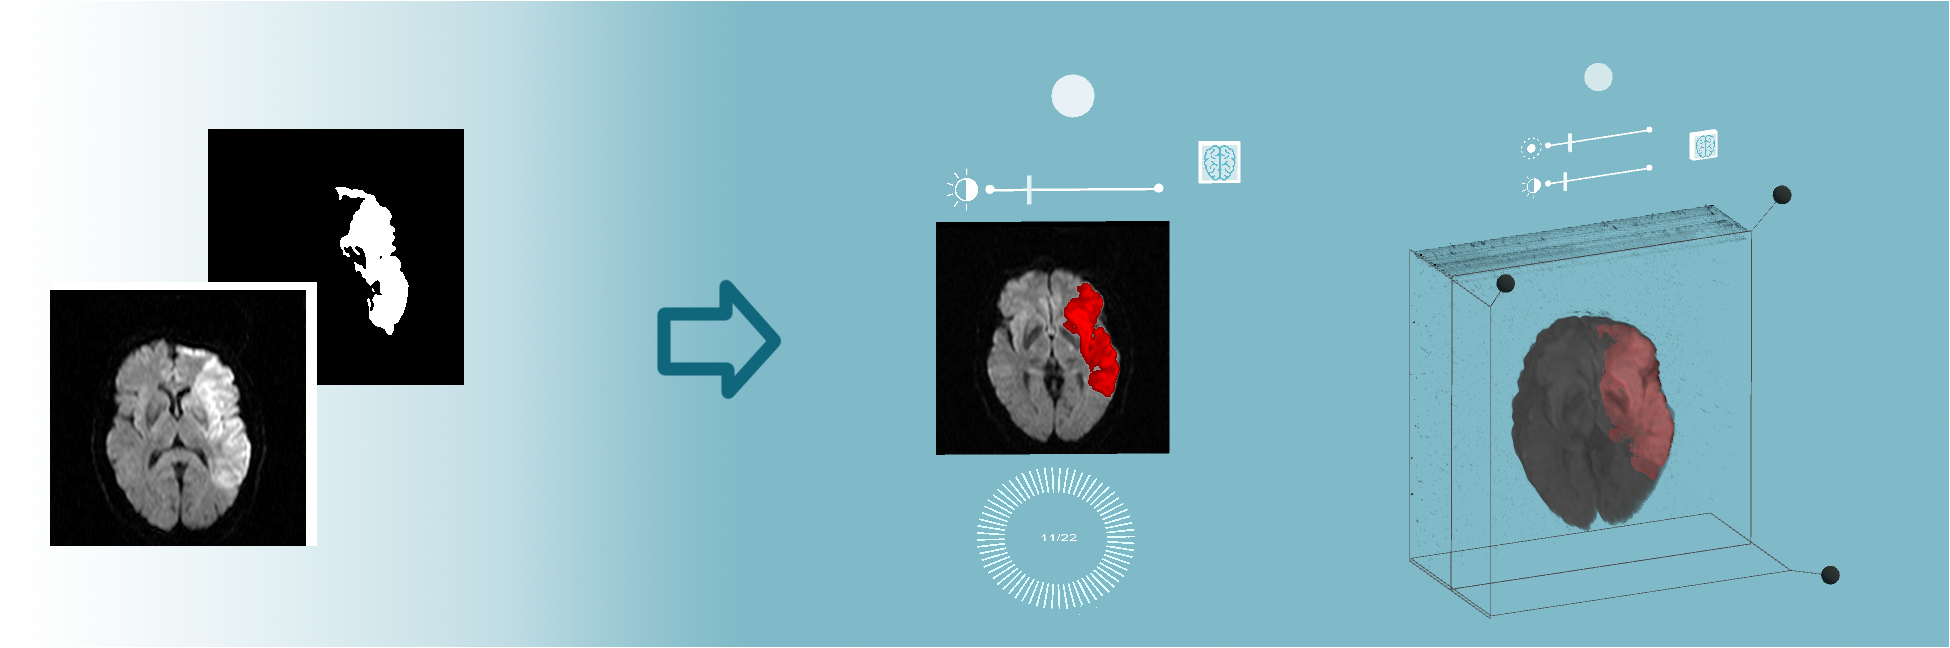
\includegraphics[width=0.3\linewidth]{images/teaser.png}
	\caption{}
	\label{img:teaser}
\end{figure}

\chapter{Einleitung}

Der Einsatz von MRTs ermöglicht es Ärzten einen Einblick in das innere des menschlichen Körpers zu erlangen, ohne diesen dabei zu verletzten. Sie erhalten Bilder innerer Organe, anhand derer sich dessen Aufbau und Funktionalität beobachten lassen. Aber auch mögliche Fehlfunktionen oder Anomalien können so erfasst werden. So können auf MRT-Scans gebrochene Knochen, innere Verletzungen oder Schlaganfälle erkannt und beurteilt werden. Im Fall von Schlaganfällen kann ein MRT aufzeigen welcher Bereich des Gehirns von diesem betroffen ist, und welchen Umfang der Schaden hat.
% Wie genau?
Um den Fall eines Patienten richtig beurteilen zu können ist es unabdingbar, dass der Arzt eine möglichst umfassende Vorstellung von der Struktur des Gehirns des Patienten und vor allem von den vom Schlaganfall betroffenen Bereichen hat. Nur wenn dies der Fall ist, kann eine sinnvolle Therapie angewandt werden.
Diese Arbeit stellt die Möglichkeit vor den Umgang mit MRT-Daten anschaulicher und intuitiver zu gestalten, um somit die Arbeit von Radiologen im Bereich der Schlaganfallbehandlung zu erleichtern und die Gesundheit ihrer Patienten zu verbessern.

\section{Motivation}
\label{motivation}

Um MRT-Scans zu studieren benutzen Ärzte in der Regel speziell dafür entwickelte Software. Diese stellt das Gehirn meist aus drei verschiedenen Blickwinkeln dar, sodass es von allen Seiten zusehen ist. Entlang dieser Achsen kann der Nutzer die Ansicht durch die Schichten des Scans bewegen. Die aktuelle Position der gerade angezeigten Schicht wird in jeder der anderen Achsenansichten farbig eingezeichnet, um dem Nutzer ein möglichst umfassendes Bild des gescannten Gehirns zu vermitteln. 
Ein Beispiel für die Oberfläche solch einer eben beschriebenen Software ist in Abbildung \ref{images/mrtSoftware} zu sehen. 
% Grundlagen?

Die zweidimensionale Ansicht, in der die Bilder vorliegen können allerdings eine falsche Vorstellung von der vorliegenden Situation schaffen. 
%Refrerenz?
Durch die Reduzierung um eine Dimension entsteht ein verzerrtes Bild des Gehirns. Die Darstellung der verschiedenen Achsen auf den Scans soll den Arzt bei der Orientierung unterstützen. Da das Gehirn allerdings durch mehrere Bilder dargestellt wird ist es diesem nicht möglich den Zustand auf einen Blick zu erfassen. Stattdessen müssen die Informationen aus zwei oder mehr Bildern im Kopf zusammengesetzt werden, was ein gewisses räumliches Vorstellungsvermögen voraussetzt. Dies ist ein kognitiver Aufwand, der Ärzte zusätzlich belastet, während sie sich darauf konzentrieren Anomalien in den Scans eines Patienten zu erkennen und einzuschätzen. 

Wird auf einem Scan ein Schlaganfall entdeckt, ist es durch die Abstraktion des Organs schwierig eine korrekte Vorstellung von der Größe und Lage des betroffenen Bereichs zu bekommen, da jeweils nur eine Schicht des Gehirns sichtbar ist. 
Eine dreidimensionale Ansicht des gescannten Gehirns würde einen sehr viel deutlicheren Einblick in den Zustand des Patienten liefern. Vor allem der vom Arzt gekennzeichnete betroffene Bereich wäre in 3D um einiges anschaulicher. Dies ist nicht nur für den behandelnden Arzt hilfreich. Durch die klare und eindeutigere Darstellung fällt es auch leichter den anderen die Situation zu erläutern. Dies trifft auf Patienten zu oder auch auf andere Ärzte, die der behandelnde Arzt eventuell in den Fall mit einbeziehen möchte.

Schließlich würde eine 3D-Darstellung auch das Verständnis in Lernzwecken begünstigen.
Da der betroffene Bereich in einer 3D-Darstellung auf einen Blick erfasst werden kann, eignet sie sich außerdem, um den direkten Vergleich zwischen zwei zuständen zu ziehen. So fiele es leichter beispielsweise die Größe des Bereichs vor und nach einer Therapie gegenüberzustellen, um deren Erfolgt zu demonstrieren oder zu beurteilen.

% UX  
% Software zum Vergleichen finden
Um die Anschaulichkeit und Plastizität der 3D-Darstellung voll zur Geltung zu bringen muss sie auch im dreidimensionalen Raum platziert werden. Eine volumetrische Darstellung der Daten in einer Bildschirmanwendung ist nur eine Projektion auf eine zweidimensionale Fläche. Die Darstellung wird dabei abstrahiert und der Nutzer kann nicht direkt mit dem Objekt interagieren.
Die Platzierung des 3D-Objekts in der dreidimensionalen Welt des Nutzers löst diese Barrieren auf. AR- und VR-Technologien ermöglichen sowohl die Visualisierung von dreidimensionalen virtuellen Objekten in der Umgebung des Nutzers, als auch die direkte Interaktion mit diesen. Diese gestaltet sich dabei auch deutlich intuitiver als die Bedienung eines Programms mit konventionellen Eingabemodulen, wie z.B. einer Maus. Das trifft vor allem auf tragbare AR-Brillen zu, deren Steuerung in der Regel ohne externe Steuerungsgeräte, wie Controller erfolgt. Dies ermöglicht eine verständliche und schnelle Bedienung,  was ungeübten Nutzern, wie z.B. einem Patienten oder Studenten zu Gute kommt. Die Nutzung der Anwendung wird dadurch zudem interessanter und unterhaltsamer.\\

Die Steuerung durch die Hände des Nutzers ist im medizinischen Bereich außerdem von besonderem Wert. So kann die Anwendung auch in sterilen Räumen oder sogar während einer Operation eingesetzt werden. In diesem Szenario kommt ein weiterer Vorteil eines tragbaren AR-Headsets zur Geltung: Durch das transparente Display kann ist es dem Nutzer möglich während der Nutzung der Anwendung seine Umgebung im Auge zu behalten. 
Eine AR-Anwendung ermöglicht es also einem Arzt während einer Operation relevante Daten abzurufen.

Durch die kabellosen, tragbaren AR-Headsets ist gleichzeitig eine höhere Mobilität gegeben, als durch einen Desktop-PC. Dadurch kann die Anwendung unabhängig von der Umgebung überall zum Einsatz kommen. 

Die Vorteile einer AR-Anwendung werden im Kapitel \ref{konzept} noch einmal erläutert.

AR-Anwendungen entwickeln sich stetig weiter und werden in der Zukunft einen immer größeren Teil des Alltags einnehmen (\citet{forbes}). Diese Entwicklung wird sich voraussichtlich auch auf den medizinischen Bereich auswirken. 
% Referenz?
Ärzte sind sich der neuen Möglichkeiten bewusst und sind daran interessiert, 
in welchen Einsatzgebieten man einen Nutzen aus diesen ziehen kann, wie \citet{holomed1} zeigen.
Eine Anwendung wie mARt eignet sich gut, um den praktischen Einsatz von AR prototypisch zu testen.

mArt bietet somit die folgenden Vorteile :

\begin{itemize}
\item 3D-Darstellung der MRT-Daten verbessert allgemeines Verständnis 
\item Direkte Interaktion mit Daten ermöglicht intuitive und ansprechende Interaktion
\item Handsteuerung und Portabilität einer AR-Anwendung ermöglichen Gebrauch im OP
\end{itemize}


\section{Zielsetzung}
% hier techniken kokretisieren

Ziel dieser Arbeit ist es, die Möglichkeiten der Darstellung von und Interaktion mit MRT-Daten in AR untersuchen. Der Fokus liegt dabei auf der Darstellung von Gehirnscans, die in der Schlaganfalldiagnose und -behandlung verwendet werden.
Hierzu soll eine prototypische Anwendung konzipiert und implementiert werden, die die eben genannten Möglichkeiten demonstriert: mARt.
Die MRT-Bilder werden innerhalb einer AR-Anwendung dreidimensional dargestellt. Außerdem soll eine möglichst intuitive Interaktion mit der Darstellung ermöglicht werden. 
Um eine nützliche Anwendung zu entwickeln, die den Anforderungen eines Einsatzes im Arbeitsfeld eines Radiologen entspricht, werden Interviews mit einem Radiologen geführt werden. Aus diesen wird dann die nötige Funktionalität der Anwendung abgeleitet. 
Die Anwendung ist nicht als einsetzbares Produkt zu verstehen sondern eher als Prototyp, der die Nützlichkeit und das Potenzial des Programms beweisen soll. Der Nutzen der Anwendung wird am Ende der Arbeit durch Nutzertests evaluiert.


\section{Struktur dieser Arbeit}

Zuerst werden im  Kapitel \ref{grundlagen} theoretische Grundlagen zu Methoden und Techniken erläutert, die für das Verständnis dieser Arbeit notwendig bzw. hilfreich sind. Weiterhin werten andere Arbeiten vorgestellt,die sich mit einem ähnlichem Thema befassen oder die inhaltlich die Thematik dieser Arbeit berühren
Um die genaue Funktionalität und Umfang der zu implementierenden Anwendung festzustellen, werden in Kapitel \ref{anforderung} die Interviews mit den bereits erwähnten Radiologen ausgewertet und daraus User Stories und schließlich eine Anforderungsliste erstellt.
Anhand dieser Anforderungen wird in Kapitel \ref{konzept} ein theoretischer Entwurf der Anwendung ausgearbeitet, indem Methoden und Techniken, sowie die Benutzung des Programms diskutiert und festlegt werden.
Die Umsetzung des entwickelten Konzeptes wird schließlich in Kapitel \ref{implementierung} beschrieben. Dabei wird auch Hürden eingegangen, die im Rahmen dieser auftraten.
Das Ergebnis der Implementierung wird in Kapitel \ref{ergebnisse} dargelegt.
Die Anwendung wird anschließend getestet und mit den zuvor gestellten Anforderungen verglichen. Die Ergebnisse werden in Kapitel \ref{evaluation} beschrieben. 
In Kapitel \ref{fazit} werden die Schwerpunkte der Arbeit noch einmal zusammengefasst und mögliche Weiterentwicklungen in der Zukunft werden diskutiert. 
 
%% Related works

\chapter{Verwandte Arbeiten}

\section{Ein Abschnitt}
% Grundlagen & verwnadte Arbeiten

\chapter{Aktueller Stand der Technik}
\label{grundlagen}
%-------------------------------------------------------------
\section{AR in der Medizin}												 %
%-------------------------------------------------------------
 %// TODO:
 Relevante Arbeiten identifizieren
 genau beschreiben: TEchniken? Unterschiede zu meiner arbeit warum relevant?
 
Der Nutzen, den AR-Anwendungen in der Medizin darstellen wurde bereits von zahlreichen Arbeiten belegt. Die Einsatzbereiche sind dabei vielfältig.
Beispielsweise stellen \citet{Voinea16} eine AR-Anwendung vor die den Lernprozess im Bereich der Biomechanik unterstützt.

\subsection{Bildgestütze medizinische Eingriffe}

Ein großer Anwendungsbereich ist der Einsatz von AR in der Ausführung und Vorbereitung von Operationen. Bei einem chirurgischen Eingriff kann für den Patienten ein hohes Risiko, eventuell sogar Lebensgefahr bestehen. Deshalb ist es wichtig, dass der operierende Arzt sich bestmöglich auf seine Aufgabe vorbereiten kann, wobei AR-Anwendungen ihn unterstützen können.
Die Kerneigenschaft von AR ist die Fähigkeit der Technologe die Umgebung des Nutzers mit zusätzlichen Informationen anzureichern. Im Rahmen einer Operation bedeutet das Daten und Bildmaterial zum Fall des Patienten anzuzeigen. Um dem Arzt bei der Orientierung während des Eingriffs zu unterstützen ist es sinnvoll ihm anatomische Bilder zur Verfügung zu stellen, die er vorher bereits studiert hat. Diese stammen meist aus zuvor erzeugten MRT-Daten, die unter Umständen weiterverarbeitet wurden. Durch AR können diese in Echtzeit an der realen Positionen angezeigt werden. 
Die folgenden Arbeiten haben sich mit der Umsetzung dieses Konzeptes beschäftigt.

% Hololens

% Andere Hardware
AR-Systeme werden genutzt um MRT-Daten während eines Eingriffs zugänglich zu machen. Während ein Patient sich in einem MR-Scanner befindet, können die MRT-Bilder direkt an den Arzt weitergeleitet werden. Dieser kann diese zur besseren Orientierung bei z.B. Injektionen nutzen. Offene MRT-Systeme (s. \ref{mrt}) ermöglichen dabei eine Abbildung der betroffenen Organe während des Eingriffs. Die Bildqualität ist allerdings deutlich schlechter als bei geschlossenen Systemen. Bei einem geschlossenen System hat der Arzt dagegen während des Scans keinen Zugang zum Patienten. Um einen MRT-gestützen Eingriff durchführen zu können werden die vorher erstellten MRT-Bilder auf den Patienten projiziert. zur Umsetzung eines Systems gibt es verschiedene Ansätze.
\citet{Fritz2012} stellen ein System vor, bei dem eines transparenten Spiegels MRT-Bilder über einen Patienten bzw. ein Modell projiziert werden. Die Visualisierung soll Ärzte bei der Nadelführung für Injektionen der Wirbelsäule unterstützen. 
\citet{khamene03} verwenden für einen ähnlichen Anwendungsdall ein HMD und projiziert die Bilder abhängig vom Blickwinkel des Arztes auf den Patienten. Das HMD wurde von \citet{khamene01} weiterentwickelt, sodass der Arzt es während einer Gehirnoperation tragen kann. Dabei wird das Körperinnere durch eine dreidimensionale Visualisierung sichtbar gemacht, die aus MRT-Bildern gewonnen wurde. 

Bildgestüzte Operationen 
\citet{fuchs98} verwenden ebenfalls ein HMD. Über dieses werden Bilder aus einer Laparoscopy auf den Patienten projiziert. (Relevanz?)
Image guided surgery :\citet{grimson99} und  \citet{KerstenOertel2013TheSO}
\citet{MISCHKOWSKI2006478}
\citet{MISCHKOWSKI2006478} untersuchen eine Bildschirm basierte AR-Anwendung, die bei Kieferoperationen zum Einsatz kommt. Mit Hilfe der Anwendung kann der Eingriff geplant werden und während der Operation hilft sie dabei, die Position des Kiefers zu überprüfen. 
\citet{Soler04} beschreiben Methoden zur Automatisierung einer dreidimensionalen Visualisierung von MRT-Bildern der Verdauungsorgane. Sowie den Einsatz von AR bei Operationen in diesem Bereich. 
\citet{GasquesRodrigues17} untersuchen die Einsatzmöglichkeiten von AR und VR im operativen medizinischen Bereich. Dazu gehört unter anderem die Entwicklung einer AR-Anwendung für die Hololens, die die Ausbildung von Ärzten in Anatomie und Operationen unterstützen soll. 
\citet{Wendt03} entwickeln eine HMD basierte AR-Anwendung, die MRT-Bilder bei Eingriffen auf den Patienten Projiziert. Die Anwendung wurde mit Bildern des Gehirns an einem Kopfphantom getestet.
\citet{Watts17} stellen ebenfalls eine AR-Anwendung vor, die Bilder auf den Körper des Patienten projiziert. Allerdings ein Projektoraufbau verwendet, sodass mehrere Betrachter gleichzeitig die Augmentierung sehen können. Wie in den meisten genannten Arbeiten werden Marker auf dem Patienten angebracht, um das Bild anzupassen.
\citet{Tabrizi15}


\subsection{Visualisierung von medizinischem Bildmaterial}

Neben der Entwicklung von AR-Sytemen, die währen eines Eingriffs verwendet werden können steht im Fokus vieler Arbeiten die Möglichkeiten der dreidimensionalen Visualisierung der Menschlichen Anatomie. Indem ein realitätsgetreues Abbild eines Organs erzeugt wird, können Diagnosen und Behandlungsmöglichkeiten erleichtert werden.

% Lesen, Referenzen?
\citet{Mangina17} stellen einen Ansatz zur Erzeugung dreidimensionalen Modellen des Herzens vor, um diese zu Lernzwecken und zur Vorbereitung auf Operationen zu verwendet. Um den Nutzen der 3D-Modelle zu maximieren werden sie in einer AR- und VR-Anwendung platziert. Die Daten die dem Modell zugrunde liegen stammen aus einem MRT-Scan.Die Arbeit verfolgt demnach ein ähnliches Ziel wie diese. 
Zur Implementierung der Anwendungen wurde die Spiele Engine Unity 3D verwendet (s. Kapite\ref{implementierung}).
Ziel der Anwendung war es eine Interaktive Lernerfahrung zu schaffen, die es dem Nutzer ermöglicht das Herz in seine verschiedenen Komponenten zu zerlegen. Für diesen Anwendungsfall wird ein Mesh des Organs benötigt, das seine Oberfläche abbildet. Die inneren Strukturen sind dabei irrelevant. Hierin unterscheidet sich  die Ansätze der beiden Arbeiten. mARt setzt den Fokus der 3D-Visualisierung auf das Innere des Gehirns.
Auf Grund der Notwendigkeit eines Meshs wurde der Marching-Cubes Algorithmus zu dessen Erzeugung eingesetzt. Dieser wird in Kapitel \ref{grundlagen} erläutert.
\citet{Mangina17_2} untersuchen die Möglichkeiten zur Erzeugung eines 3D Models aus MRT-Daten genauer.

Ein weiter Ansatz zur Erzeuggung von 3D-Modellen des Herzens wird von \citet{SORENSEN2001193} beschrieben. Hier soll das Modell ebenfalls in eine VR-Anwendung integriert werden, um von Ärzten als Vorbereitung auf eine operation genutzt werden. 
Auch hier soll ein Mesh des Organs erzeugt werden. Die Generierung soll dabei möglichst automatisierbar sein.  Hierzu werden zuerst die Konturen aus den MRT-Bildern extrahiert. Dies resultiert in ein Gitter aus Konturen die dann algorithmisch durch polygone verbunden werden. 
Für die Anwendung, in der das Modell dargestellt wird wurde ein damals erhältliches VR-System eingesetzt, das mit einem HMD und zwei Controllern funktionierte. 
Durch die Controller wurde eine eine einfache aber intuitive Interaktion umgesetzt. Der Nutzer kann das Modell Vergrößern und rotieren.  

\citet{Calvin01} projizieren 2D und 3D Gehirnbilder aus MRTs auf Kopfphantom für Gehirnoperationen.

%-------------------------------------------------------------
\section{MRT}
\label{mrt}												 %
%-------------------------------------------------------------

Die Abkürzung MRT steht für Magnetresonanztomographie. Das bildgebende Verfahren, das auch Kernspintomografie genannt wird, wird in der Radiologie verwendet, um Abbildungen innerer Organe zu erzeugen. Während der Durchführung einer MRT wird der Patient in ein MRT-System geschoben, das einer großen Röhre gleicht. Er sollte sich für die Dauer des MRTs möglichst wenig bewegen, um klare Bilder zu erhalten.
Es gibt offene und geschlossene MRT-Systeme. Offene Systeme haben die Form eines C, das den Patienten umgibt und werden daher auch C-Systeme genannt. in einem geschlossenen ist der Patient dagegen vollständig von einer Röhre umgeben. Die Bildqualität ist bei geschlossenen Systemen deutlich besser.

Im folgenden wird die Funktionsweise eines MRT-Scans erläutert, diese wurde von \citet{weishaupt09} beschrieben.

\begin{figure}
	\centering
	%https://www.flickr.com/photos/11304375@N07/3081315619/
	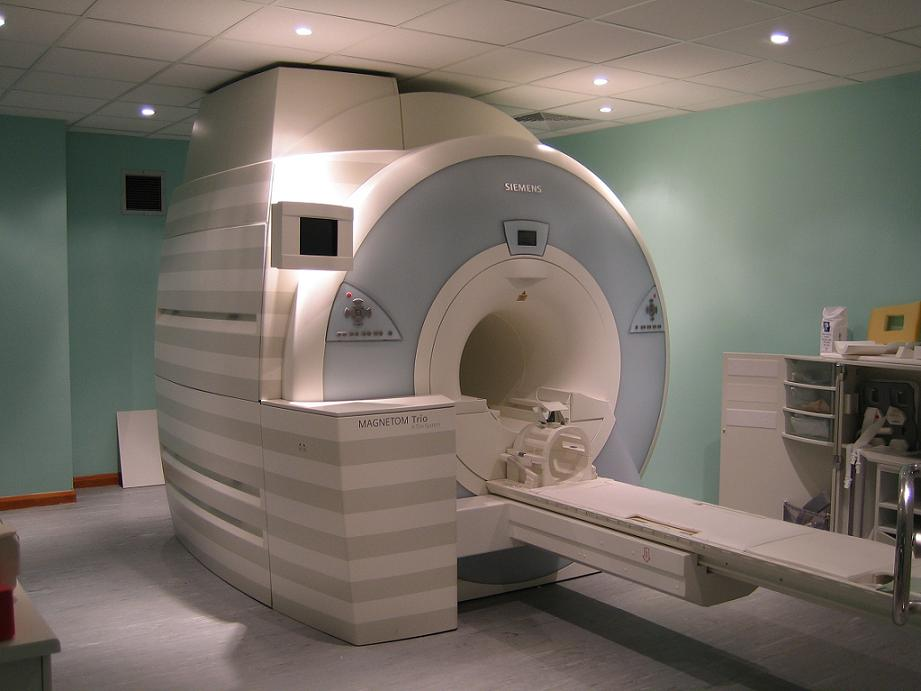
\includegraphics[width=0.5\linewidth]{images/mri.jpg}
	\caption{Ein geschlossenes MRT-Gerät. Auf die Liege im vorderen Bereich legt sich ein Patient, der dann während des Scans in die Röhre geschoben wird. }
	\label{img:mri}
\end{figure}
 	
\subsection{Verfahren}

Um die inneren Organe eines Patienten zu visualisieren, werden kleinste Teilchen seines Körpers in Bewegung versetzt, die gemessen werden kann. Im Falle einer MRT handelt es sich dabei um Wasserstoffprotonen. Diese haben eine Eigendrehung um sich selbst, den sogenannten Kernspin. Durch ihre positive Ladung, die durch den Kernspin in Bewegung ist, besitzen die Protonen weiterhin ein eigenes Magnetfeld, welches messbar ist. 
Während einer MRT wird mit einer Hochfrequenz-Spule (HF-Spule), die in dem MRT-System verbaut ist um den Körper des Patienten ein Magnetfeld erzeugt. Die Kernspin-Achsen der Wasserstoffprotonen richten sich an diesem aus. Anschließend wird in das Magnetfeld ein Hochfrequenzimpuls, die Larmorfrequenz eingestrahlt. Durch diesen Impuls findet eine Synchronisation der Protonen statt, wobei einige um 180° gedreht werden. Kurz danach laufen die Protonen wieder auseinander und richten sich wieder am Magnetfeld aus. 
Dadurch, dass alle Protonen in dieselbe Richtung zeigen (phasengleich sind), verstärken sie gegenseitig das Signal, dass sie abgeben. Das Signal wird schwächer, sobald sie wieder auseinander laufen (Dephasierung).
Die Zeit, die die Protonen brauchen, um sich wieder am Magnetfeld auszurichten wird als Relaxtionzeit bezeichnet. Dabei wird zwischen T1- und T2-Relaxtion unterschieden.
Die Relaxionszeit ist dabei abhängig von der Zusammensetzung des umgebenden Gewebes. Das gemessene MR-Signal, das durch diese beeinflusst wird, ist also für verschiedene Gewebearten verschieden stark.

\subsection{Erfassung dreidimensionaler Daten}

Mit dem eben beschriebenen Verfahren werden jeweils Werte auf der XY-Ebene erfasst. Um dreidimensionale Daten zu erhalten wird diese XY-Ebene entlang der Z-Achse Verschoben. Das Gehirn wird auf diese Weise in einzelne Schichten unterteilt, von denen jede ein zweidimensionales Bild ist.
Diese Unterteilung in Schichten wird erreicht, indem weitere Spulen verwendet werden, die ein ein zusätzliches Magnetfeld (Gradientenfeld) erzeugen, welches das erste Magnetfeld inhomogen macht. Dementsprechend fällt es zu einer Seite hin ab, was sich durch einen Gradienten, den Z-Gradienten, beschreiben lässt. So kann jeder Z-Schicht eine bestimmte Stärke im Magnetfeld zugewiesen und einzelne Schichten durch die Verwendung bestimmter Frequenzen angeregt werden. In Abbildung \ref{img:zGradient} ist schematisch dargestellt, wie die Schichten entlang des Z-Gradienten hintereinander liegen und eine von ihnen angeregt wird.
Es wird immer nur eine Schicht auf einmal gescannt und verarbeitet.

\begin{figure}
	\centering
	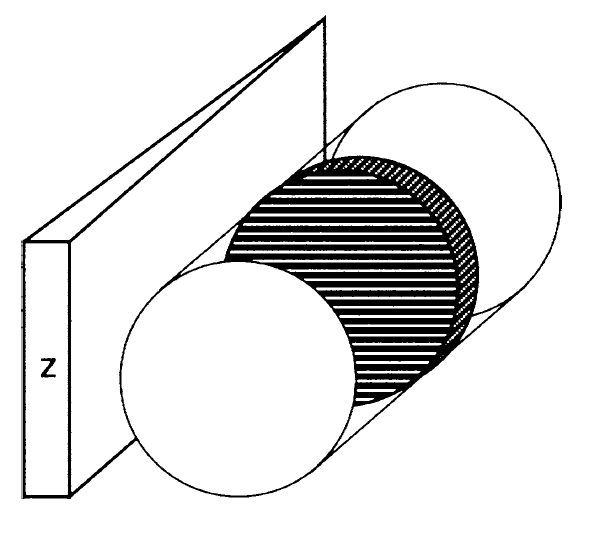
\includegraphics[width=0.3\linewidth]{images/zGradientMrt.png}
	\caption{Darstellung der Schichten während eines MRT-Scans. Links ist der abfallende Z-Gradient zu sehen, daneben drei verschiedene Schichten (Ellipsen). Durch das inhomogene Magnetfeld, kann genau eine Schicht mit einer bestimmten Frequenz angeregt werden. Die ausgewählte Schicht ist hier schraffiert. \citet{weishaupt09}}
	\label{img:zGradient}
\end{figure}


Die X- und Y-Werte einer Schicht repräsentieren allerdings nicht, wie bei einem Bild Koordinaten, die der Anordnung der jeweils betrachteten Punkte in der Welt entsprechen. Stattdessen bildet der X-Wert die Frequenz und der Y-Wert die Phase ab. Wie für den Z-Wert werden auch hier Gradienten gebildet und auf das Magnetfeld gelegt. Der X-Gradient verläuft von links nach rechts und sorgt dafür, dass die Larmorfrequenz in dieser Richtung zunimmt, sodass die jeder Punkt seine eigene Frequenz hat.Der Y-Gradient, der senkrecht verläuft, beeinflusst auf dieselbe Weise die Phasen einer Schicht. Er wird dabei nur kurz nach dem Einstrahlen des Hochfrequenz-Impulses eingeschaltet, wenn sich die Protonen bereits ausgerichtet haben.

Für jeden Punkt gibt es also eine Magnetfeldstärke (Z), eine Frequenz (X) und eine Phase (Y). Diese Werte aller Punkte werden in einer Matrix gespeichert, die K-Raum genannt wird. Die Matrix entspricht allerdings noch nicht der bildlichen Darstellung, die angestrebt wird, da die Werte eine andere Bedeutung haben. ? Deshalb werden sie mit Hilfe der Fouriertransformation in lesbare Bilddaten umgewandelt, die die entsprechenden Organe schichtenweise abbilden. 
\citet{weishaupt09}

\subsection{Abgrenzung CT}
Eine von der Durchführung ähnliche Methode zur Abbildung des Körperinneren, ist die Computer-Tomographie. Die Verfahren unterscheiden sich jedoch. Denn bei einer CT wird der Patient schichtenweise geröntgt. D.h. sein Körper wird mit Röntgenstrahlung beschossen, die je nach Gewebe, auf das sie treffen unterschiedlich stark abgeschwächt werden, was dann gemessen wird. Die so entstandenen "Querschnitte" des Körpers werden anschließend mit Hilfe eines Computers zu einem dreidimensionalen Bild zusammengesetzt. 

Die CT ist deutlich kürzer als eine MRT. Deshalb wird sie oft bei Notfällen verwendet. Allerdings wird der Patient dabei auch der Belastung von radioaktiver Strahlung ausgesetzt, die stärker ist als beim normalen Röntgen. Außerdem ist können Weichteile mit einer MRT besser darstellt werden. Sie eignet sich also mehr zur Untersuchung des Gehirns.

Die resultierenden Daten sind allerdings genau wie beim MRT Volumendaten und können demnach ähnlich verarbeitet werden.

REFERENZ

\subsection{Datenformate}

MRT-Bilder werden meist in Dateiformaten gespeichert, die in der Medizin üblich sind. Dazu gehören das NIfTI-Format (Neuroimaging Informatics Technology Initiative) sowie das DICOM-Format (Digital Imaging and Communications in Medicine), welches z.B. neben den Bildern auch Patientendaten speichert.

Das NIfTI-Format wurde 2003 von der Data Format Working Group (DFWG) als Alternative zum vorherigen Analyze 7.5-Format entwickelt, das Probleme mit der Orientierung der Daten aufwies. Durch fehlende Informationen, wie die Daten im Raum liegen war oft nicht klar, welche Gehirnhälfte die rechte und welche die linke ist. Deshalb wird im NIfTI-Format in Header festgelegt, wie die Koordinaten der Voxel auf Weltkoordinaten abgebildet sind. Beide Formate werden im Bereich des Neuroimaging verwendet.
Bilderinformationen werden bei ersterem in einer einzigen Daten mit der Endung .nii gespeichert, während Analyze 7.5 die Daten in zwei verschiedenen Dateien abgelegt hat: Einer Header-Datei und einer, die die Volumendaten enthalten hat. Um mit dem Analyze-Format kompatibel zu bleiben besitzen auch NIfTI-Dateien einen 348 Byte Header.
 
Dem Header folgen die Volumedaten des Scans. Es ist möglich bis zu sieben Dimensionen in der Datei abzulegen. Die ersten drei sind dabei für die X-,Y- und Z-Dimensionen des Volumens reserviert.
% https://brainder.org/2012/09/23/the-nifti-file-format/

DICOM bezeichnet nicht nur das Dateiformat in dem medizinische Bilder gespeichert werden, sondern auch legt auch ein Kommunikationsprotokoll zum Austausch von medizinischen Daten fest. Der DICOM-Standart wird in den meisten medizinischen Einrichtungen verwendet, um medizinische Bilddaten zu speichern und auszutauschen.
Der DICOM-Standart besteht aus 16 Teilen.
%https://hpi.de/fileadmin/user_upload/fachgebiete/meinel/papers/Old_Source/TR_Med_Bildverarbeitung.pdf

Wie bereits erwähnt speichert eine DICOM-Datei neben den Bilddaten weitere Informationen. Dazu können eine ID oder der Patientenname zählen, die als Attribute des DICOM-Objektes hinterlegt werden. 
..

%// TODO:
DICOM genauer beshcreiben
Header vergleichen
vorteile nachteilel

MRT-Bilder werden außerhalb des medizinischen Umfelds allerdings auch in anderen Formaten gespeichert. 
Ein Beispiel dafür ist das PVM-Format, das zum Speichern von volumetrischen Daten genutzt wird. Das Format geht davon aus, dass das Volumen aus quadratischen Voxeln besteht und enthält die Voxelwerte und Größeninformationen über das Volumen.
% http://paulbourke.net/dataformats/pvm/

Die Daten können weiterhin in herkömmlichen Bildformaten, wie JPEG oder PNG gespeichert werden. Dabei entspricht dann eine Bilddatei einer Schicht des Scans. 
 
 \citet{Larobina13} stellen medizinische Bilddateiformate vor.
 \citet{graham05} beschrieben DICOM Format und DICOM Viewer.
%16 bit int images, pvm ? Standart?

%------------------------------------------------------
\section{Volumendaten}							  	  %
%------------------------------------------------------

Ein wichtiger Aspekt dieser Arbeit ist die dreidimensionale Visualisierung von MRT-Daten. Deshalb soll an dieser Stelle auf einige grundlegende Aspekte und Begriffe im Zusammenhang mit Volumendaten eingegangen werden. Da das Gehirn durch einen MRT-Scan dreidimensional erfasst wird, liegen die MRT-Daten als Volumendaten vor. Die Daten werden durch ein Skalarfeld repräsentiert. Ein Skalarfeld ist ein Sammlung von Skalarwerten, die in einem Raum verteilt sind. Durch eine Funktion kann jedem Punkt im Raum ein Skalarwert zugewiesen werden. Im Fall von Volumendaten handelt es sich um ein dreidimensionales Skalarfeld. D.h. die Skalarwerte sind innerhalb eines Würfels angeordnet für jeden Skalarwert existieren X-, Y- und Z-Koordinaten, die dessen Position beschreiben. 
Diese Punkte aus denen sich der Volumen-Würfel zusammensetzt werden auch Voxel genannt. Ähnlich wie Pixel in zweidimensionalen Bildern stellen sie die kleinsten Teilchen in einem Volumen dar. 
Die Skalarwerte werden auch als Isowerte des Volumens bezeichnet bei MRT-Daten bildet jeder Wert eine Graustufe ab und liegt damit in dem Bereich von 0-255. 
Über das Volumen verteilt haben benachbarte Werte oft ähnliche Isowerte. Eine Gruppe dieser Werte wird als Isofläche bezeichnet. Isoflächen innerhalb eines Volumens entsprechen oft tatsächlichen Oberflächen des darzustellenden Objektes. Durch das Vergleichen benachbarter Werte ist es also möglich Oberflächen von Objekten zu ermittlen (siehe \ref{marchingCubes}). 

Volumendaten werden oft in 3D-Texturen gespeichert. Diese funktionieren auf dieselbe Weise wie 2D-Texturen und entsprechen, wie beschrieben der Vorstellung eines Würfels. Die Textur besitzt Texturkoordinaten in drei Dimensionen und 

Die Verfahren zur dreidimensionalen Visualisierung von MRT-Daten lassen sich in drei Bereiche teilen: Multiplanar Reformation (MPR), Surface Rendering (SR), und (direktes) Volume Rendering (VR). \citet{Zhang10} In den folgenden Abschnitten werden diese verfahren erläutert.

%------------------------------------------------------
\section{Volume Rendering}							  %
%------------------------------------------------------
%https://developer.nvidia.com/gpugems/GPUGems/gpugems_ch39.html
% Bezug zu Motivation
Wie in Kapitel \ref{motivation} erläutert, sollen die MRT-Bilder, die der Neurologe untersucht in mARt als dreidimensionales Volumen dargestellt werden. Volume Rendering bezeichnet die Darstellung eines dreidimensionalen Volumens, meist durch ein Skalarfeld repräsentiert, auf einer zweidimensionalen Bild. MRT-Bilder, die in Graustufen vorliegen bilden ein solches Skalarfeld. 

Dadurch, dass das Volumen aus Voxeln gebildet wird, gibt es keine Oberfläche, die das abzubildende Objekt beschreibt. Die Darstellung erfolgt deshalb anhand eines optischen Modells. Jedem Wert im Datensatz werden dazu optische Eigenschaften zugewiesen, im Allgemeinen Farbe und Opazität. Indem Strahlen durch das Volumen geschossen werden, werden diese Eigenschaften mit einander verrechnet, was schließlich zur Abbildung des gesamten Volumen führt. Diese Technik wird im Abschnitt \ref{rayCasting} genauer beschrieben.
Die optischen Eigenschaften eines Voxels sind abhängig von seinem Isowert, sowie der verwendeten Transferfunktion und dem Shading. 

Im Folgenden werden grundlegende Techniken, sowie verschiedene Verfahren der Umsetzung des Volume Rendering erläutert.

\citet{Kaufman03}
\citet{kniss02}
%//TODO: 
Beispielarbeiten recherchieren, beschreiben
REFERENZEN-> GPU GEMS

\subsection{Klassifikation}

Die Klassifikation von Voxeln bestimmt deren optische Eigenschaften in Abhängigkeit zu ihrem Isowert. Diese beschreiben, die Aufnahme und Abgabe von Licht eines einzelnen Voxels. Die Abgabe von Licht manifestiert sich aus der Sicht des Betrachters in der Farbe eines Voxels. Die Aufnahme äußert sich in dem Grad der Opazität. Durch die Unterschiede in Farbe und Opazität einzelner Voxel, werden verschiedene Bereichen, wie z.B. Gewebestrukturen voneinander unterscheidbar. Die Qualität des gerenderten Bildes hängt zu einem großen Teil von der Klassifikation ab.Oft wird eine Transferfunktion verwendet, um Voxel zu klassifizieren. Auf diese wird im folgenden Abschnitt näher eingegangen. 

Das Ergebnis einer Klassifikation hängt von dem Zeitpunkt ab, zu dem diese durchgeführt wird. Sie kann vor oder nach der Interpolation der Volumendaten durchlaufen werden.

Die Daten müssen interpoliert werden, da das Volumen wie mehrfach beschrieben in einzelnen Werten vorliegt. Der Raum zwischen diesen Werten ist nicht definiert. Um ein zusammenhängendes Volumen darstellen zu können muss also eine Interpolation zwischen den Werten stattfinden. Diese wird in der Regel durch die Verwendung eines Filters bzw. einer Convolution umgesetzt. Sir findet während des Rasterisierungsschrittes statt?

Werden die Voxel vor dieser Interpolation klassifiziert, wird dies als Pre-Klassifikation bezeichnet. Dabei werden jedem Isowert die entsprechenden Eigenschaften zugewiesen. Die Zwischen den Voxeln bestehenden Lücken werden aufgefüllt, indem zwischen den Farb- und Opazitätswerten interpoliert wird. 
Im Gegensatz dazu, werden bei der Post-Klassifakation zuerst alle Skalarwerte durchlaufen und der Bereich zwischen ihnen durch Interpolation der Isowerte überbrückt. Erst danach werden den Werten durch die Klassifizierung Eigenschaften zugewiesen. Der Unterschied besteht also darin, ob die Erzeugung von neuen Werten, die die vorhandenen verbinden auf Basis der Voxelwerte oder der Werte ihrer Eigenschaften stattfindet. \citet{Hadwiger06}



Obwohl die Vorgehensweisen also beinahe gleich sind, führen sie doch zu deutlich unterschiedlichen Ergebnissen. Die Interpolation der Voxeleigenschaften bei der Pre-Klassifizierung führt zu Artefaktbildung, da die lediglich Eigenschaftswerte "gestreckt" werden, ohne die Formen des Volumens zu beachten. Bei der Post-Klassifikation werden die fehlenden Daten anhand der Struktur des Objektes erzeugt. Dies führt zu einer deutlich klareren Darstellung des Volumens. Der Vergleich ist in \ref{img:prepost} veranschaulicht.

\begin{figure}
	\centering
	%http://schorsch.efi.fh-nuernberg.de/roettger/index.php/VolumeRendering/Pre-AndPost-Classification
	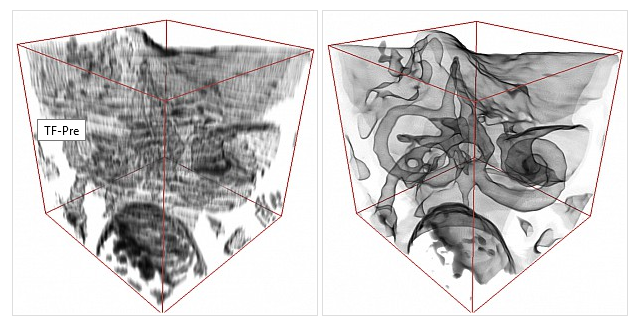
\includegraphics[width=0.7\linewidth]{images/prepostclassification.png}
	\caption{Vergleich zweier Volumen Renderings mit unterschiedlicher Klassifizierung. Durch die Verwendung von Pre-Klassifikation (links) entstehen Artefakte. Die Post-Klassifikation (rechts) liefert eine bessere Darstellung des Volumens.}
	\label{img:repost}
\end{figure}

Welche Interpolation? Wann?

Pre-Integrierte Tandferfunktion ? 

//TODO:
Klassifikationen unterscheiden

\subsection{Transferfunktion}

Transferfunktionen werden verwendet, um verschiedenen Bereichen bzw. Beschaffenheiten eines Objektes verschiedene Farben und Opazitäten zu geben. Unterschiedliche Geweben können auf diese Weise eingefärbt oder ausgeblendet werden. In der Umsetzung besteht eine Transferfunktion meistens aus einer Textur, aus der für jeden Isowert eine Farbe und Opazität gelesen werden kann. Die Textur kann dabei eindimensional sein, wenn als Index lediglich der Isowert des Voxels verwendet wird. Für eine bessere Unterscheidung der Gewebe eines Objektes können allerdings auch multidimensionale Transferfunktionen eingesetzt werden. Hierbei werden neben dem Isowert z.B. auch der Betrag des Gradienten des jeweiligen Voxels als Koordinaten für die Transfer-Textur verwendet. In Abbildung \ref{img:transferfunction} ist der Unterschied zwischen der Verwendung von ein- und zweidimensionalen Transferfunktionen verdeutlicht. Der Zugriff auf die Transferfunktion erfolgt genauso wie bei anderen Texturen. Im folgenden Codebeispiel ist demonstriert, wie in einem Shader auf die 3D-Textur des Volumens und die 1D-Textur der Transferfunktion zugegriffen wird. \citet{Fernando04}

\begin{minted}[mathescape,
               linenos,
               numbersep=5pt,
               gobble=2,
               frame=lines,
               framesep=2mm]{csharp}
void main(sampler3D _Volume,
          sampler1D _TransferTexture,
          float3 texCoord : TEXCOORD0,
          float4 color : COLOR)
{
  // Der Isowert des Volumens wird für die aktuelle Position ausgelesen
  float isoValue = tex3D(_Volume, texCoord);
  // Die Farbe des Volumens wird für die aktuelle Position ausgelesen
  color = tex1D(_TransferTexture, isoValue);
}
\end{minted}

Eine gut Transferfunktion zu implementieren ist sehr schwierig, da die korrekten Werte oft nur durch Ausprobieren gefunden werden können und von dem jeweiligen Datensatz abhängen. Teilweise werden Widgets eingesetzt, die es den Nutzer erlauben eine Transferfunktion zu erstellen, die direkt auf ein gerendertes Volumen angewandt wird.
\citet{salama06} und \citet{Knig99} beschreiben die Entwicklung von Benutzeroberflächen zur Erstellung von Transferfunktionen.

\begin{figure}
	\centering
	%http://developer.download.nvidia.com/books/HTML/gpugems/gpugems_ch39.html
	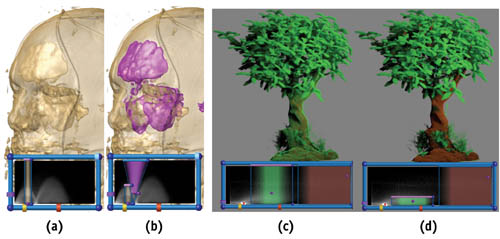
\includegraphics[width=0.7\linewidth]{images/transferfunction.jpg}
	\caption{Abbildung zweier gerenderter Volumen und der jeweils dafür verwendeten Transferfunktion. In den Darstellungen a) und c) wurde eine eindimensionale Transferfunktion verwendet. b) und c) benutzen zweidimensionale Tranfserfunktionen, wodurch verschiedene Bereiche des Volumens anders eingefärbt sind. }
	\label{img:phong}
\end{figure}

Die Verwendung einer Transferfunktion ist Teil der Klassifikation von Voxeln, da über die Transferfunktion definiert ist, welche Isowerte welchem Gewebe entsprechen.

\subsection{Beleuchtung}
\label{beleuchtung}

Um dem gerenderten Objekt einen möglichst plastischen Eindruck zu verleihen und es somit realistischer aussehen zu lassen ist es sinnvoll dieses zu beleuchten. 
Die Beleuchtung wird in in der Regel durch einen Shader implementiert. Jeder Voxel wird dabei einzeln nach der Anwendung der Transfertextur geshadet, sodass dessen Eigenschaften zusätzlich zur dieser verändern werden. Es können verschiedene Modelle zur Beleuchtung verwendet werden. Außerdem ist zwischen lokaler und globaler Beleuchtung zu unterscheiden.


Die lokale Beleuchtung betrachtet nur die Beziehung des Lichtes zu dem Objekt. Dabei bleiben Beleuchtungseffekte, wie Schatten, den das Volumen wirft oder indirekte Beleuchtung außen vor. Zudem ist das Beleuchtungsmodell auf Oberflächen ausgelegt und nicht auf ein Volumen. 

Eine realistischere Beleuchtung bietet daher die globale Beleuchtung mit Schatten und indirekter Beleuchtung.
Um Schatten im Volumen darzustellen, muss bestimmt werden, wie viel Licht bei einem Voxel ankommt, nachdem das Licht andere diesen umgebende Voxel passiert hat und dadurch abgeschwächt wurde. 
Dazu könnte ein Schatten-Volumen erstellt werden, indem jeder Voxel aus Sicht des Lichts gerendert wird, welches mit den Werten aus der Transfertextur verrechnet wird. Dieses Vorgehen ist allerdings unperformant und liefert unschöne Ergebnisse.\citet{Fernando04}
Stattdessen wird das Volumen durch Texture Slicing aus der GPU (?) in Schichten unterteilt. Jede Schicht dann wird jeweils aus Sicht der Kamera und des Lichtes gerendert. Jedes der beiden gerenderten Bilder wird in einem 2D-Textur-Buffer gespeichert. 
Die Lage der Schichten wird durch die die Winkelhalbierende des Blickrichtungswinkels und des Lichtrichtungswinkels bestimmt. Dadurch treffen beide Vektoren im selben Winkel auf die Schichten. Abhängig von dem Skalarprodukt der Vektoren kann auch die Inverse des Blickwinkels verwendet werden. Das Skalarprodukt bestimmt außerdem, ob die Schichten aus Kamerasicht von hinten nach vorne oder von vorne nach hinten durchlaufen werden. Während für das Licht immer von vorne nach hinten gerendert wird.
Die Position der Vektoren und der winkelhalbierenden Schicht ist in Abbildung \ref{img:halfAngleSlice} dargestellt.

\begin{figure}
	\centering
	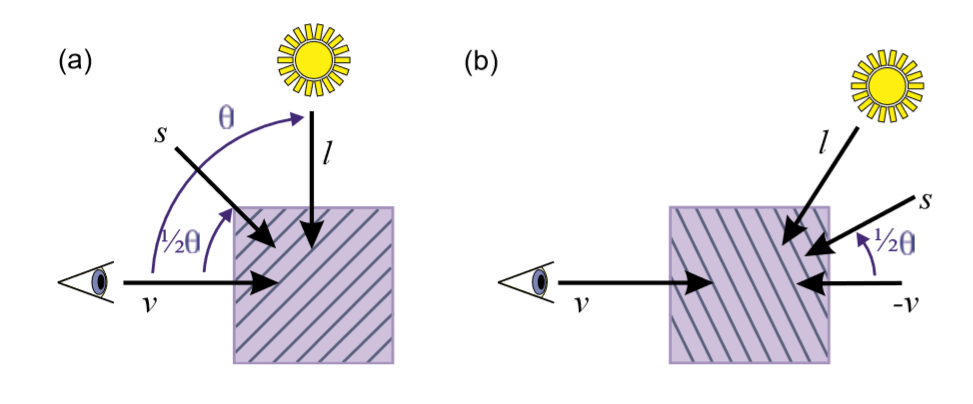
\includegraphics[width=0.7\linewidth]{images/halfAngleSlice.png}
	\caption{Durch Bestimmung der Winkelhalbierenden des Licht- und Kamerarichtungsvektors, wird die Lage der Schichten bestimmt, die sowohl aus Licht- als auch Kamerasicht gerendert werden. Bei einem Skalarprodukt $>=0$ wird der Kameravektor verwendet (a), bei einem negativen Skalarprodukt dessen Inverse (b). \citet{Hadwiger06}}
	\label{img:halfAngleSlice}
\end{figure}


Jede Schicht wird dann zuerst aus Sicht der Kamera gerendert. Die aus Lichtsicht gerenderte vorhergehende Schicht ist dabei bereits bekannt. So kann jeder Punkt des Kamera-Textur-Buffers mit jedem des Licht-Textur-Buffers der vorherigen Schicht verrechnet werden. Dabei wird durch den Wert des Kamera-Buffers die Farbe und Opazität aus der Transferfunktion gelesen. Die entsprechende Farbe wird dann mit dem Wert aus dem Licht-Buffer multipliziert. Die so berechnete Schicht wird wieder in den Kamera-Buffer geschrieben. Dann wird die aktuelle Schicht aus Sicht der Lichtquelle in den Licht-Buffer gerendert, um diesen für die nächste Schicht zu verwenden.
Für jede Schicht wird ein eigener Pass durchlaufen.
\citet{Hadwiger06}
\citet{Fernando04}

//TODO:
IndirekteBeleuchtung/Scattering? /Translucency  
Indirekte Beleuchtung entsteht, wenn ein Objekt von Licht getroffen wird, das vorher von woanders reflektiert wurde. Bei einem Volumen beschreibt es dabei in der Regel die Streuung von Licht innerhalb des Volumens. Dabei wird dass Licht, nachdem es auf das Objekt getroffen ist, von dessen Inneren reflektiert, während es in dieses eindringt. Dies ist der Fall bei Objekten aus transluzentem Material, wie z.B. Wachs oder Haut.

\citet{hansen03} stellen ein Shading Modell vor, dass realistisches Rendering von transluzenten Materialien erlaubt.

Phasenfunktion 

Die globale Beleuchtung ist somit von der Umsetzung her deutlich komplexer. Bietet allerdings auch mehr Plastizität und Realismus. Dies wird in Abbildung \ref{img:localGlobalIll} deutlich, in der die Ergebnisse der beiden Vorgehensweisen gegenübergestellt sind.

\citet{Jnsson14} untersuchen derzeit verwendete Beleuchtungmethoden von Volumen.

\begin{figure}
	\centering
	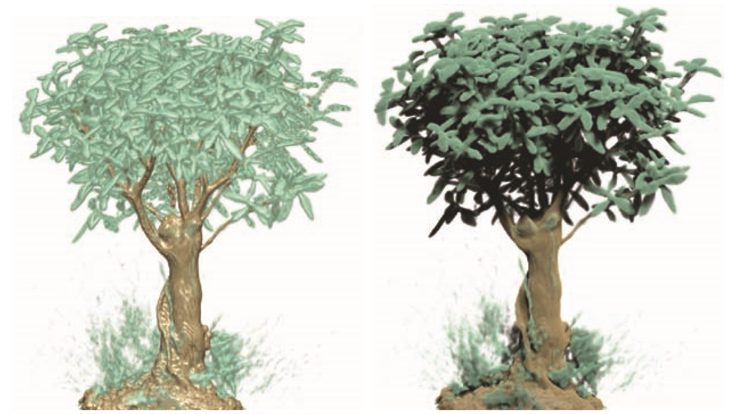
\includegraphics[width=0.7\linewidth]{images/localGlobalIllumination.png}
	\caption{Vergleich zweier Volumen, die mit lokaler Oberflächenbeleuchtung (links) und direkter Beleuchtung und Schatten (rechts) gerendert wurden. \citet{Hadwiger06}}
	\label{img:localGlobalIll}
\end{figure}

Bei einer lokalen Beleuchtung der einzelnen Voxel kommt meist das Phong-Beleuchtungsmodell zum Einsatz. 

\begin{figure}
	\centering
	%https://commons.wikimedia.org/wiki/File:Phong_components_version_4.png
	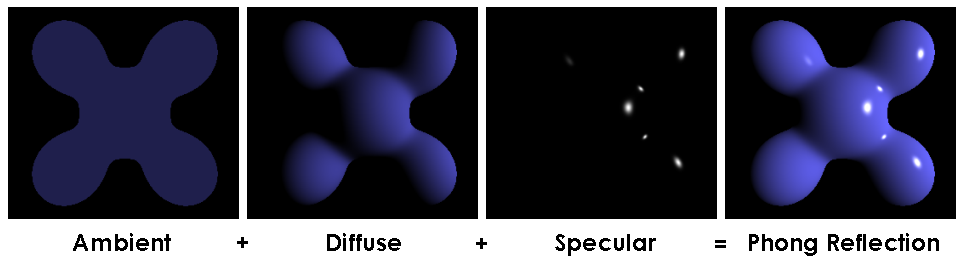
\includegraphics[width=0.7\linewidth]{images/Phong_components_version_4.png}
	\caption{Visuelle Aufteilung des Phon-Beleuchtungsmodells in seine drei Komponenten. Die Farbe pro Pixel wird für jede Komponente einzeln berechnet und die Komponenten schließlich zusammen addiert, um die Beleuchtung zu erhalten. }
	\label{img:phong}
\end{figure}

% PHONG
Das Modell setzt sich aus drei Komponenten zusammen: Der ambienten und der diffusen Beleuchtung, sowie der spiegelnden Reflexion. Diese werden aufeinander addiert und ergeben so das Phong-Beleuchtungsmodell.  In Abbildung \ref{img:phong} ist zu sehen, wie die einzelnen Komponenten isoliert aussehen und wie sie in Kombination die vollständige Beleuchtung ergeben.
Die folgende Formel beschreibt, wie die Beleuchtung berechnet wird. Die Terme zwischen den $+$-Zeichen stehen für die Berechnungen der genannten Komponenten.

$I = k_{a}+I_{L}k_{d}(\vec{l}\cdot\vec{n})+I_{L}k_{s}(\vec{r}\cdot\vec{v})^n$

$I$ ist dabei die Farbe des beleuchteten Punktes, die bei Verwendung einer Transferfunktion durch diese bestimmt wird. $\vec{n}$ ist die Normale und $\vec{l}$ ist der Richtungsvektor zum Licht. $I_{l}$ ist die Intensität des Lichtes. $\vec{r}$ und $\vec{v}$ sind der Reflexionsvektor des einfallenden Lichtes und der Richtungsvektor zur Kamera. Weiterhin setzt sich die Formel aus dem ambienten, diffusen und spiegelndem Koeffizienten $k_{a}$, $k_{d}$ und $k_{s}$ zusammen. Hinzu kommt der Exponent $n$, der konstant ist und die Stärke der Reflexion bestimmt. (?)

\citet{phong75}
//TODO: Andere Beleuchtungsformen? -> Vergleich

\subsection{Gradientenberechnung}

Um die in \ref{beleuchtung} erläuterte Beleuchtung umzusetzen, müssen wie beschrieben die Normalen der einzelnen Voxel bekannt sein. Da es die Voxel allerdings keine Oberfläche bilden, besitzen sie auch keine Normalen. Als Ersatz können stattdessen die Gradienten der Voxel verwendet werden. Diese beschreiben die Wertveränderung in der Umgebung eines Voxels und zeigen dabei auf die Größte Veränderung. Benachbarte Voxel mit ähnlichen Isowerten bilden eine Isofläche, die durch die Gradienten beschrieben wird. 
% ??

Zur Berechnung der Gradienten können verschiedene Verfahren eingesetzt werden. Der Unterschied in der Berechnung liegt vor allem in dem Zeitpunkt zu dem diese ausgeführt werden. Gradienten können entweder vor dem Start des Programmes berechnet werden oder zur Laufzeit. 

Ist ersteres der Fall werden die Gradienten in den meisten Fällen per Pixel mit Hilfe der Finite-Differenzen-Methode berechnet. 
Dabei wird jeweils die Differenz zwischen dem Isowert eines Voxels und den Voxeln in seiner festgelegten Umgebung gebildet. Dies lässt sich als folgende Formel ausdrücken: 

$
\Delta f(x,y,z)\approx \frac{1}{2h}
\left ( \begin{matrix}
f(x + h, y, z) - f(x - h, y, z)\\ 
f(x, y + h, z) - f(x, y - h, z)\\ 
f(x, y, z + h) - f(x, y, z - h)
\end{matrix} \right )
$

//TODO:
Convolution?
On´The fly gradientenberechnung
genau vorstellen
Vergleich der versch. formen -> BUCH

\citet{Correa11} haben verschiedene Methoden zur Bestimmung von Gradienten verglichen.

Segmentierung

\subsection{Komposition}

Komposition bezeichnet die Verrechung einzelner Voxelwerte. Abhängig von der Blickrichtung der Kamera beeinflussen die Eigenschaften eines Wertes das Aussehen anderer Werte um ihn herum, z.B. bei zwei Voxeln, die hintereinander liegen. Um die Endgültige Farbe eines Pixels zu erhalten werden die Werte von hintereinander liegenden Voxlen in der Regel auf addiert. Hierbei ist es von Relevanz, in welcher Reihenfolge die Werte durchlaufen werden. Wird das Volumen von vorne nach hinten durchlaufen, erfolgt die Komposition wie folgt:

$\hat{C}_{i}=(1-\hat{A}_{i-1})C_{i}+\hat{C}_{i-1}$

$\hat{A}_{i}=(1-\hat{A}_{i-1})A_{i}+\hat{A}_{i-1}$

Wobei $\hat{C}_{i}$ die Farbe und $\hat{A}_{i}$ die Transparenz der Farbe des vordersten Voxels ist.
Sollen die Werte von hinten nach vorne addiert werden, wird dies durch die folgende Formel beschrieben.

$\hat{C}_{i}=C_{i}+(1-\hat{A}_{i})\hat{C}_{i+1}$

$\hat{A}_{i}=A_{i}+(1-\hat{A}_{i})\hat{A}_{i+1}$

Die Komposition erfolgt für jeden Strahl am Ende des Renderingprozesses. Die Eigenschaften des Voxels können in dessen Verlauf verändert werden. Beispielsweise durch die Verwendung einer Transferfunktion oder eines Shaders.


\section{Volume Rendering Methoden}
//TODO:
Splatting??

\subsection{Volumetrisches Ray-Casting}
\label{rayCasting}

\begin{figure}
	\centering
	%https://de.wikipedia.org/wiki/Datei:Volume_Ray_Casting-de.svg
	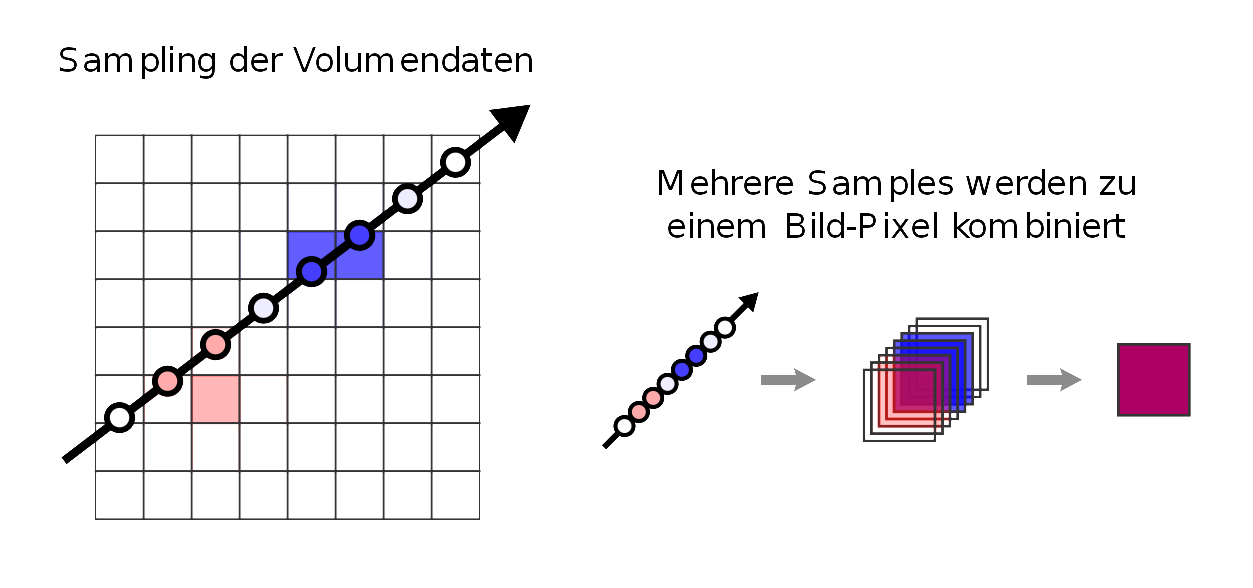
\includegraphics[width=0.7\linewidth]{images/rayCasting.png}
	\caption{Schematische Darstellung des volumetrischen Ray Castings. Ein Strahl (Pfeil) durchläuft das Volumen (Würfel). Die Eigenschaften (Farbe und Opazität) jedes Voxels, der passiert wird werden zusammengerechnet, um die Farbe eines Pixels des Renderings zu erhalten.}
	\label{img:rayCasting}
\end{figure}

\textbf{Ray-Casting} ist eine bekannte Rendering-Methode, die auch beim Rendern von 3D-Szenen zur Anwendung kommt die keine Volumendaten enthalten.
In diesem Fall werden von der Position der Kamera für jeden Pixel Strahlen in die Szene geschossen. Für jeden Strahl wird dann errechnet, ob dieser die Oberfläche eines der Objekte in der Szene schneidet. Ist dies der Fall, wird der betreffende Pixel in der Farbe des Objektes eingefärbt, wobei der verwendete Shader diese beeinflusst. Es wird außerdem berücksichtigt, welche Länge der Strahl zu dem Schnittpunkt hat, da nur der Eintrittspunkt relevant ist.
Weiterhin existieren die Techniken Ray-Tracing und Ray-Marching, die ebenfalls auf der Kollision zwischen Strahlen und Objekten beruhen.
Beim \textbf{Ray-Tracing} werden dabei neben dem ursprünglichen Strahl, der das Objelt trifft noch weitere berechnet, die durch die gesamte Szene laufen können um z.B. die Reflexion von Objekten aufeinander zu ermitteln. 
\textbf{Ray-Marching} ist eine schnellere Version des Ray-Castings. Hier wird der Schnittpunkt von Strahl und Oberfläche nicht genau kalkuliert. Stattdessen wird entlang des Strahls in kleiner werdenden Abständen jeweils ein einzelner Punkt betrachtet. Für diesen Punkt wird lediglich geprüft, ob er sich bereits innerhalb des Objektes befindet oder nicht. Der erste Punkt, auf den dies zutrifft wird als Schnittpunkt angesehen. Obwohl diese Berechnung etwas weniger genau ist, ist wie bereits gesagt schneller als Ray-Casting.

%Ray-Casting bzw. Ray-Marching wird auch zum Rendering von Volumen benutzt.
Bei beiden Verfahren muss allerdings die Oberfläche bzw. die Form des Objektes bekannt sein, um bestimmen zu können, wann der Strahl in sie eintritt. Dies ist bei Volumendaten in der Regel nicht gegeben, da nicht zur das Objekt selbst, sondern auch dessen Umgebung darin gespeichert sind. Weiterhin werden durch die eben beschriebenen Prozesse nur die Oberflächen der Objekte gerendert, nicht aber ihr Inneres.

Hier liegt der Unterschied zum Rendering von Volumen. In diesem Fall werden beide Verfahren quasi vereint. \textbf{Volumetrisches Ray-Casting} und volumetrisches Ray-Marching bezeichnen deshalb ein und dasselbe. Auch hier werden dabei Strahlen von der Kamera in die Szene geschossen. Um das Volumen zu rendern sind davon nur die Strahlen relevant, die das Volumen treffen. Und auch von diesen wird nur der Teil des Strahls berücksichtigt, der innerhalb der umgebenden Geometrie liegt. Für jeden Strahl Ein- und Austrittspunkt errechnet. Innerhalb der Geometrie werden jetzt entlang des Strahls in bestimmten Abständen Voxel betrachtet. Für jeden Voxel wird ein Farb- und Alphawert bestimmt und die Werte werden abhängig von der Komposition von hinten nach vorne oder von vorne nach hinten aufeinander addiert. Die Summen der Werte ergeben so eine dreidimensionale Darstellung des Volumens aus der Sicht der Kamera. Der Vorgang ist in Abbildung \ref{img:rayCasting} veranschaulicht.


\subsection{Texture Based Volume Rendering}

Beim texturbasierten Rendering von Volumen wird eine dreidimensionale Darstellung erzeugt indem viele Texturen aufeinander geschichtet werden, die dann mit Alpha Blending übereinander geblendet werden. Dazu wird für jede Schicht ein Querschnitt durch das Volumen gemacht, auf den dann mit Hilfe von Texture Mapping die Textur gerendert wird.
Die Form und Ausrichtung der Querschnitte wird dadurch bestimmt auf welche Art die Volumendaten vorliegen. In Abbildung \ref{img:2D3DTex} wird der Unterschied verdeutlicht. Handelt es sich um zweidimensionale Texturen,  richten sich die Querschnitte am Volumen aus. Innerhalb eines Würfel sind sie also quadratisch. Damit das Volumen aus verschiedenen Blickwinkeln betrachtet werden kann, wird für jede der Hauptsichtachsen ein Stapel mit Texturen erstellt. Zwischen den Stapeln wird gewechselt, sobald sich der Betrachtungswinkel ändert. Dadurch wird verhindert, dass der Betrachter zwischen zwei Texturen durchsehen kann, wenn diese annähernd parallel zu seiner Blickrichtung stehen. Dies ist in Abbildung \ref{img:textureBased} dargestellt.

\begin{figure}
	\centering
	%https://www.evl.uic.edu/aej/524/lecture06.html
	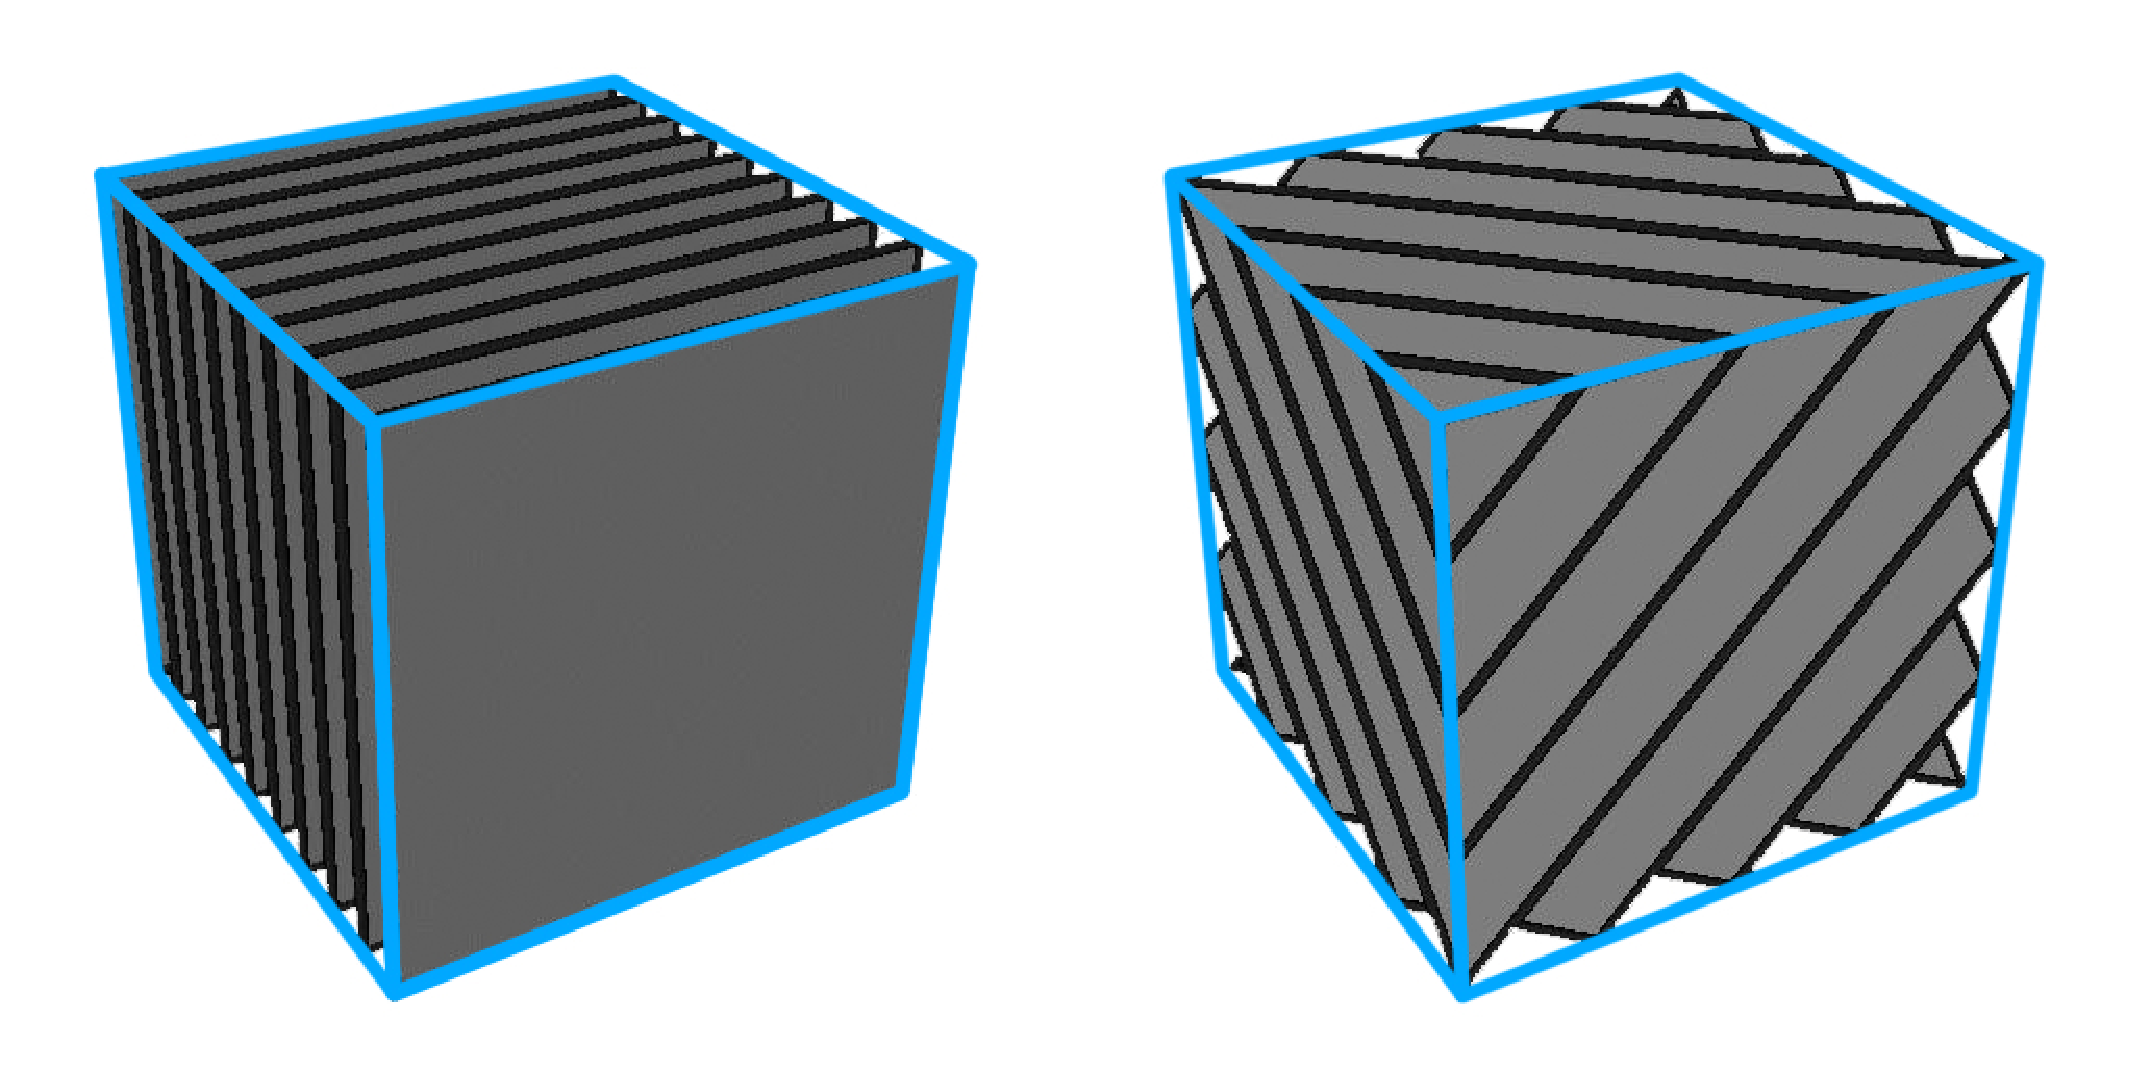
\includegraphics[width=0.7\linewidth]{images/texture_2d3d.pdf}
	\caption{Links: Texturen beim werden entlang des Volumens ausgerichtet. Recht: Texturen werden entlang des Blickwinkels ausgerichtet.}
	\label{img:2D3DTex}
\end{figure}

\begin{figure}
	\centering
	%https://www.researchgate.net/figure/Object-aligned-slice-stacks-with-2d-texture-mapping_fig1_226214561
	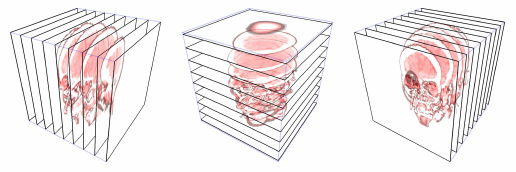
\includegraphics[width=0.7\linewidth]{images/textureStacks.png}
	\caption{Texturen werden als Stapel in der 	XY-, YZ- und XZ-Ebene angeordnet.}
	\label{img:textureBased}
\end{figure}

Liegen die Daten als 3D-Texturen vor, verlaufen die Querschnitte entlang der Sichtachse. Dazu werden sogenannte Proxy Geometrien erzeugt, Polygone, die einen Querschnitt beschreiben. Auf diesen Proxy Geometrien wird dann die Textur erstellt, indem die entsprechenden Volumendaten abgefragt werden. Dadurch, dass die Querschnitte an der Sichtachse ausgerichtet sind, ist nur ein Texturstapel notwendig. 


https://dl.acm.org/citation.cfm?id=329138

// TODO:
implementierung auf der grfikkarte mit 2d texuren nachteil: nur flächen nicht geometrie
3d texure based? 	
kann man shaden?

\subsection{Shear-Warp}

Shear-Warp verfolgt den selben Ansatz wie das Ray-Casting. Anstatt die Strahlen allerdings von der tatsächlichen Kameraposition aus zu verschießen, werden die Strahlen orthogonal zu den Volumenschichten in das Volumen gefeuert. Auf diese Weise wird die Berechnung der Strahlen und die Komposition der Darstellung deutlich beschleunigt. 
Damit auch bei einem nicht orthogonalen Blickwinkel das Volumen korrekt dargestellt wird, wird vor dem Ray Casting eine vom Blickwinkel abhängige Scherung auf die Volumendaten angewandt. In Abbildung \ref{img:shearwarp} ist Dargestellt, wie die Scherung die einzelnen Schichten entsprechend des Blickwinkels verschiebt, um einen orthogonalen Einfallswinkel zu simulieren. 
Das durch das Ray Casting entstandene Bild wird zunächst in einen Buffer gerendered. Durch die Scherung ist das Bild zu diesem Zeitpunkt noch verzerrt. Deshalb wird es anschließend noch einmal transformiert, sodass eine korrekte Abbildung des Volumens auf die Bildschirmebene projiziert wird. In Abbildung \ref{img:shearwarp} ist zu sehen, wie das gerenderte Bild vor und nach der Transformation aussieht. 

Shear-Warp vereint damit die Bildqualität des Ray-Castings, ist aber dabei um einiges schneller.

\begin{figure}
	\centering
	%http://citeseerx.ist.psu.edu/viewdoc/download;jsessionid=97AC0E2CDFD635B2917DF8DF86E99224?doi=10.1.1.548.9543&rep=rep1&type=pdf
	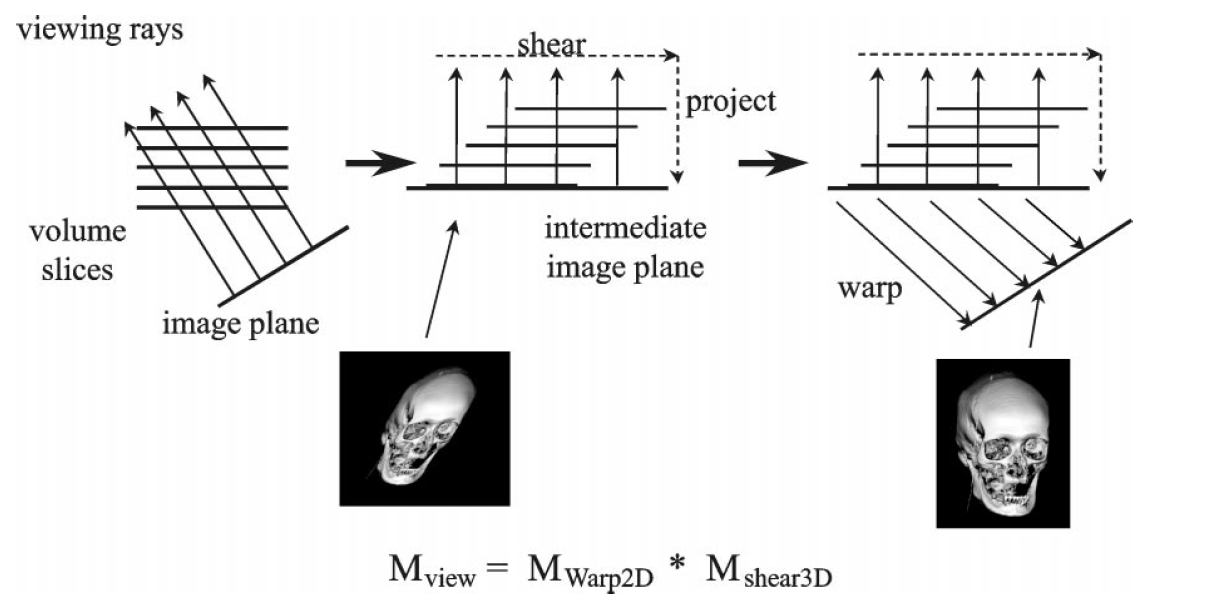
\includegraphics[width=0.7\linewidth]{images/shearwarp.png}
	\caption{Shear-Warp Verfahren. Rechts: Ohne Verschiebung würden die Strahlen der Bildebene schräg auf das Volumen treffen. Mitte: Die Schichten des Volumen werden verschoben, sodass die Strahlen orthogonal darauf treffen. Das resultierende Bild ist verzerrt. Rechts: Das verzerrte Bild wird transformiert, um das Volumen korrekt darzustellen.}
	\label{img:shearwarp}
\end{figure}

%-------------------------------------------------------------
\section{Beispiele für Volume Rendering Implementiertungen}
%-------------------------------------------------------------

Volume Rendering Techniken werden von verschiedenen Programmen und Arbeiten zur 3D-Visualisierung von MRT-Daten eingesetzt.

Beispiele für Volume Rendering Software sind \textit{MRIcroGL} von \citet{MRIcroGL} und \textit{Voreen}, entwickelt von \citet{voreen}. Die Programme erlauben dabei die Manipulation der Transferfunktion. Ersteres ermöglicht es außerdem bestimmte Bereiche zu markieren und kann durch eigene Skripte erweitert werden.
Die im späteren Abschnitt \ref{radiologieSoftware} genannte MRT-Viewer Software besitzt ebenfalls die Funktionalität die Daten in 3D darzustellen.

Um Volume Rendering spezifisch in Unity zu umzusetzen, existieren die kostenpflichtige Unity-Erweiterung textit{Volume Viewer Pro} von \citet{volumeViewerPro} sowie das Unity-Plugin \textit{Unity® Volume Rendering} von \citet{volumeRenderingUnity}. Beide nutzen Volume Ray Casting zur Darstellung von 3D-Daten und ermöglichen dem Nutzer das Erstellen eine Transferfunktion über eine Benutzeroberfläche, um das Volumen zu kolorieren. textit{Volume Viewer Pro} bietet weiterhin das Hervorheben von Bereichen durch ein Overlay, das Laden von NIfTI- und DICOM-Dateien und einige weitere Manipulationsmöglichkeiten. 

Eine der frühesten Arbeiten, die Volume Rendering Techniken vorstellen stammt von \citet{Drebin88}.

\citet{Kruger03} stellen Methoden zur Beschleunigung von Volume Rendering vor.
\citet{Marsalek08} implementieren Volume Ray Casting mit CUDA (Compute Unified Device Architecture) von \citet{cuda}, um den Rendering Prozess zu optimieren.

\citet{Kutter08} beschäftigen sich mit der Optimierung von Volume Rendering durch ein AR-HMD. Das Rendering soll interaktiv sein und von den Händen des Nutzers verdeckt werden können.

Vermehrt wird heutzutage Path Tracing oder Monte-Carlo-Raytracing zur Visualisierung von Volumen verwendet. Dabei handelt es sich um ein Verfahren ähnlich dem Ray Tracing, bei dem zufällig Strahlen in eine Szene geschossen werden, wobei ihr "Pfad" in der Szene verfolgt wird , der durch Reflexion und Absorption, sowie bei Volumen, Streuung bestimmt wird. Auf diese Weise wird eine globale Beleuchtung der Szene erzeugt. Die Technik wird vor allem zum rendern von nicht-körperlichen Volumen, wie Wolken oder Rauch eingesetzt. (?) 
\citet{Fong17} beschreiben Volume Rendering unter Verwendung von Path Tracing, vobei der Fokus auf dessen Einsatz in der Produktion liegt.

%-------------------------------------------------------------
\section{Oberflächen Generierung (Weitere Methoden zur dreidimensionalen Darstellung von MRT-Daten)}		 %
%-------------------------------------------------------------
% Bsp
Wie in Kapitel \ref{motivation} beschrieben wurde, bietet eine 3D-Darstellung von MRT-Bildern einige Vorteile gegenüber einer Betrachtung der Daten in 2D. 
% Kann man das belegen?
Auf Grund dieser Tatsache gab es im Laufe der Zeit verschiedene Ansätze zur Umsetzung einer dreidimensionalen Darstellungsweise. 
Im Folgenden werden diese erläutert. 

% Vor- und Nachteile Tabelle?


\subsection{Marching Cubes}
\label{marchingCubes}
%https://developer.nvidia.com/gpugems/GPUGems3/gpugems3_ch01.html

Das Marching Cubes Verfahren wird eingesetzt, um eine Polygonenoberfläche zu erzeugen, die ein volumetrisches Objekt visualisiert. 
Der Visualisierung liegen Volumendaten, die in Form eines Skalarfeldes vorliegen zu Grunde.
Die Idee hinter dem Algorithmus ist, dass es zwischen den Voxeln, die innerhalb und außerhalb eines Objektes liegen eine Grenze gibt, die die Oberfläche des Objektes bildet. Diese Grenze gilt es zu finden. 
Die Werte der Voxel, werden dabei als Dichtewerte angesehen. Voxel innerhalb der Grenze haben eine Dichte, die außerhalb eine andere. Demnach kann ein Schwellenwert definiert werden, der die beiden Wertebereiche voneinander trennt.
Um die Grenze zwischen den Voxeln zu ermitteln, werden diese zunächst in Würfel aufgeteilt, woher auch der Name des Verfahrens stammt. Immer vier benachbarte Voxel bilden dabei einen Würfel.  

Die Vorstellung einer Grenze zwischen den Voxeln lässt sich auf die Würfel übertragen. Dabei liegt dann ein bestimmter Teil der Würfel des Volumens mit allen Eckpunkten innerhalb und ein bestimmter Teil außerhalb des Objektes. Diese Würfel liegen nicht auf der Grenze und alle ihre Eckpunkte haben jeweils ähnliche Werte. Andererseits gibt es Würfel, durch die die Grenze verläuft. Die Eckpunkte dieser Würfel können sich in ihren Werten stark unterscheiden, da jeweils ein Punkt zum Inneren und ein anderer zum Äußeren des Objektes gehören kann. 

Um also die Oberfläche zu erzeugen, die das gesamte Volumen aufteilt, wird jeder Würfel zuerst einzeln betrachtet und es wird ermittelt, ob und wie die Polygonfläche diesen einzelnen Würfel aufteilt.  Da diese Teilung auch einzelne Eckpunkte betreffen kann, setzt sich diese Oberfläche aus dreieckigen Polygonen zusammen. ?

Die Anzahl an Möglichkeiten einen Würfel aufzuteilen lässt sich errechnen. Für jeden der acht Eckpunkte des Würfels gilt eine von zwei Möglichkeiten: Entweder befindet er sich unter der Oberfläche und damit im Objekt oder eben nicht. Demnach ergeben sich für alle Punkte zusammen $2^8=256$ mögliche Fälle der Aufteilung. \citet{aigner07} Durch in Betracht ziehen von Symmetrie, könnten diese auf 15 verschiedene Möglichkeiten reduziert werden, die in Abbildung \ref{img:marchingCubes} dargestellt sind. Der Fall, dass die Eckpunkte gar nicht getrennt werden ist dabei berücksichtigt. 

\begin{figure}
	\centering
	%https://en.wikipedia.org/wiki/Marching_cubes#/media/File:MarchingCubes.svg
	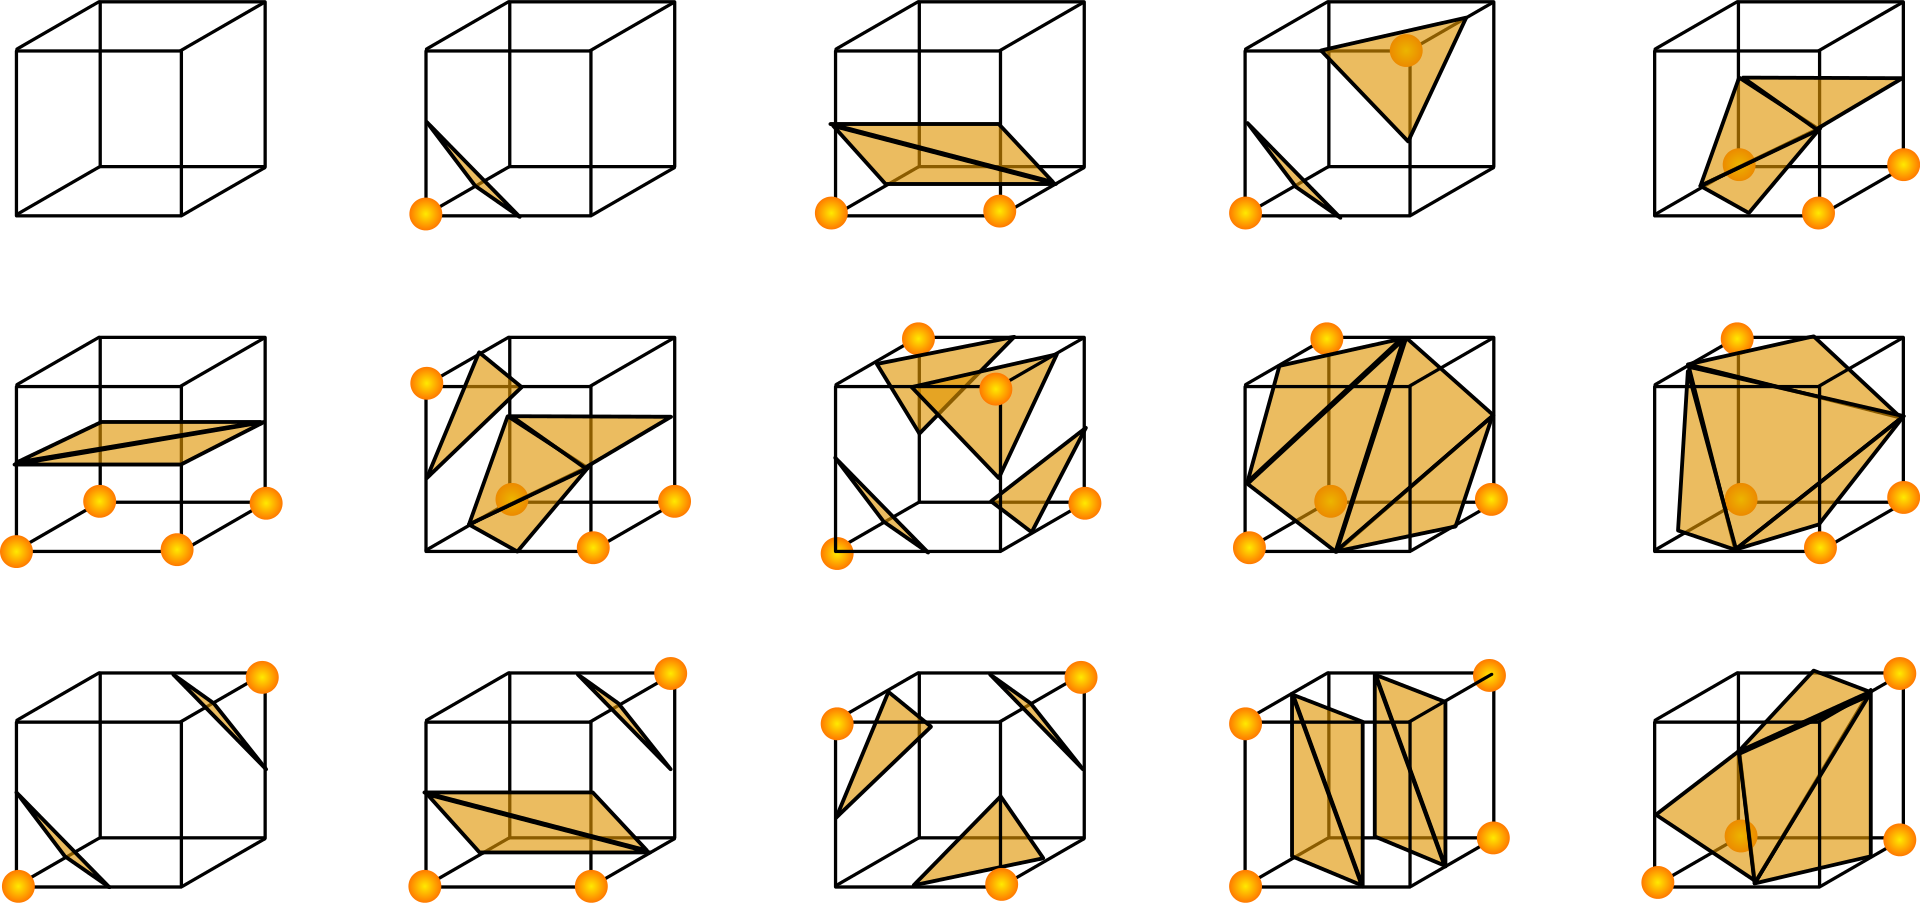
\includegraphics[width=0.7\linewidth]{images/MarchingCubes.png}
	\caption{Die 15 verschiedenen Möglichkeiten, wie eine Polygonfläche einen Würfel in zwei Bereiche teilen kann.}
	\label{img:marchingCubes}
\end{figure}

Bei der Implementierung des Algorithmus werden nun alle 256 Teilungsmöglichkeiten eines Würfels in einer Look-up-Tabelle gespeichert. Um auszulesen, welcher Fall auf den momentan betrachteten Würfel zutrifft, bedarf es eines Indexes. 
Der Index ist eine achtstellige Binärzahl. Sie wird ermittelt, indem für jeden der acht Eckpunkte des Würfels geprüft wird, ob er unter dem Schwellenwert liegt, der die Unterscheidung zwischen Innen und Außen definiert oder nicht. Die Ergebnisse der Prüfung, die durch 1 oder 0 repräsentiert werden, werden aneinander gefügt. Nach der Prüfung aller Eckpunkte ist so ein achtstelliger Index entstanden. 

Durch die Verwendung dieses Index und der Tabelle lässt sich so auslesen, wie die Polygone in dem Würfel liegen. Damit ist auch bekannt, auf welchen Würfelkanten sich deren Vertices befinden. Für die Erzeugung einer Oberfläche muss weiterhin die genaue Position des Vertex auf der jeweiligen Kante ermittelt werden. Dies geschieht durch lineare Interpolation zwischen den Werten der Würfel-Eckpunkte, zwischen denen die betreffende Kante verläuft. ??
Auf die selbe Weise wird für jeden Vertex der Polygone dessen Normale berechnet, indem die Normalen der Eckpunkte interpoliert werden.

Nach und nach werden so für jeden Voxel-Würfel Polygone berechnet, die in einer Liste gespeichert und schließlich gezeichnet werden.

Der Marching Cubes Algorithmus wird häufig zur prozeduralen Erzeugung von Terrain eingesetzt. In diesem Fall ist es entscheidend, wie die Dichtewerte des Volumens generiert werden. Bei der Visualisierung von medizinischen Daten, wie MRT-Bildern werden die Bilddaten als Eingabewerte genommen.

\citet{Lorensen87}

Beschleunigung durch Unterstützung der Grafikkarte??

Erweiterungen/ Abwandlungen
%https://dl.acm.org/citation.cfm?id=3264776

%https://www.researchgate.net/publication/279205507_A_BRIEF_REVIEW_OF_SURFACE_MESHING_IN_MEDICAL_IMAGES_FOR_BIOMEDICAL_COMPUTING_AND_VISUALIZATION

%-------------------------------------------------------------
\section{Vergleich der Methoden im Überblick}											 %
%-------------------------------------------------------------
\begin{table}
\centering
\begin{tabular}{lrrrr}
\toprule
Vergleich von Methoden zur 3D Darstellung von Volumendaten\\  
\midrule 
Methode & Ergebnis & Komplexität & Vorteile & Nachteile \\ 
\midrule 
Volumerisches Ray-Casting & Rendering &  & & \\
Shear-Warp & Redering & 8,20 & sehr schnell& schlechtere Bildqualität, benötigt viel Speicher\\
2D-Texturbasiertes Volume Rendering & Redering  & 10,00 & schnell, wird auch von alten Grafikkarten unterstützt, benötigt nur bilinieare Interpolation & Artefakte, wenn aus 45° Winkel gesehen; Abstände zwischen Texturen ist abhängig von Blickrichtung \\ 
3D-Texturbasiertes Volume Rendering & Redering  & 10,0 & keine Artefakte durch Blickwinkel; Abstand zwischen Texturen konstant & langsamer durch trilineare Interpolation; Grafikkarte braucht 3D Texturen Unterstützung\\ 
Marching Cubes & 3D-Mesh der Bestandteile des Gehirns  & 10,00 & 0 &\\ 
\bottomrule
\end{tabular}
\caption{Description of the table}\label{volumeRenderingVergleich}
\end{table}

//TODO
Tabelle
%-------------------------------------------------------------
\section{AR und VR (MR?)}									 %
%-------------------------------------------------------------
Occluded Display 

\subsection{Augmented Reality}

Der Begriff der \textit{Augemented Reality} (AR), also \textit{Erweiterte Realität} beschreibt die Idee, dass die physisch vorhandene Welt, die einen Nutzer umgibt angereichert wird mit zusätzlichen digitalen Inhalten. Dies geschieht z.B. indem wahrgenommene Gegenstände von virtuell erzeugten Objekten überlagert werden. 
Laut \citet{azuma97} zeichnet sich eine AR-Anwendung durch folgende Eigenschaften aus:

\begin{itemize}
\item Kombiniert reale und virtuelle Realität
\item Ist in Echtzeit interaktiv
\item 3D-Objekte existieren in dreidimensionaler Realität
\end{itemize}

AR und VR verbindet eine ähnliche Geschichte. Die frühesten VR-Systeme waren nach heutiger Definition AR-Systeme.
%Geshcihte?
Auch einige AR-HMDs funktionieren mit Stereoskopie. Die eben genannten Definition lässt allerdings auch andere Systeme zu. Tatsächlich gibt es eine Vielzahl von AR-Systemen. 
Beispielsweise kann eine AR-Anwendung mit oder manche ohne einen Bildschirm konzipiert werden, der die Augmentierung darstellt. Im letzteren Fall werden dann meist Beamer o.Ä. verwendet, um die Objekte in die reale Welt zu projizieren. 
Die Mehrzahl von AR-Software verwendet wahrscheinlich allerdings Bildschirme. %Warum?
Aber auch hier gibt es verschiedene Lösungsansätze. Dies betrifft zum einen die Positionierung des Bildschirms. Dieser kann direkt vor dem Auge des Nutzers, in der Welt oder in einem tragbaren Endgerät platziert werden.
Weiterhin können Bildschirme durchsichtig oder undurchsichtig sein. Handelt es sich um einen durchsichtigen Bildschirm, wird darauf nur die Augmentierung dargestellt. Des Vorteil hierbei ist, dass der seine Umgebung größtenteils unverfälscht wahrnehmen kann. Damit ist aber gleichzeitig der Kontrast zu den nicht unbedingt realitätsnahen 3D-Objekten größer.
Bei undurchsichtigen Bildschirmen nimmt eine Kamera die Umgebung auf und gibt sie augmentiert auf dem Bildschirm aus. Diese Technik wird z.B. verwendet wenn AR-Anwendungen für Smartphones oder Tablets entwickelt werden. In Abbildung \ref{img:ARPhone} ist dargestellt, wie eine solche Anwendung auf einem Smartphone aussieht.

\begin{figure}
	\centering
	%https://commons.wikimedia.org/wiki/File:App_iSkull,_an_augmented_human_skull.jpg
	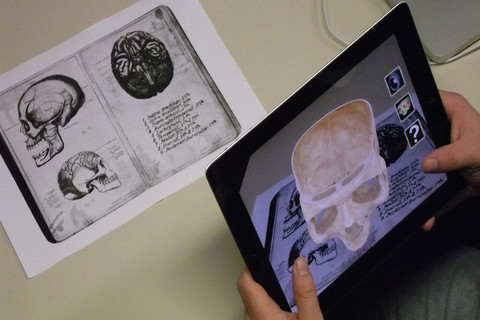
\includegraphics[width=0.5\linewidth]{images/App_iSkull,_an_augmented_human_skull.jpg}
	\caption{Eine tabletbasierte AR-Anwendung, die auf einem Marker des 3D-Modell  eines Schädels projiziert.}
	\label{img:ARMarker}
\end{figure}

Alle Techniken haben gemeinsam, dass eine Kamera Teil des Systems ist, die die Umgebung des Nutzers aufnimmt. Dadurch werden Tiefen- und Bildinformationen gesammelt. Durch die Auswertung dieser und anderer Informationen, wie z.B. GPS- oder Wlan-Daten, können 3D-Objekte korrekt mit der Umgebung in Beziehung gesetzt werden. So ist es möglich ein virtuelles Objekt auf oder hinter ein reales zu stellen. Durch ein möglichst umfassendes Verständnis des umgebenden Raumes ist es auch möglich, dass die Elemente der erweiterten Realität in der realen Welt an der richtigen Stelle platziert werden und dort auch bleiben.
Alternativ dazu können am gewünschten Ort Markierungen gesetzt werden, die das System erkennt und somit genau dort das 3D-Modell darstellen kann. Solche Marker können verschieden aussehen. Oft werden komplexe weiße Muster dafür verwendet, weil diese gut zu identifizieren und schwer zu verwechseln sind. In Abbildung \ref{img:ARMarker} ist ein 3D-Objekt zu sehen, dass auf einem Marker platziert wurde. 

Zurzeit gibt es verschiedene AR-Systeme auf dem Markt, die sich teilweise in ihrer Funktionsweise unterscheiden. Die wichtigsten sind hier aufgezählt.

Smartphones. Wie bereits erwähnt können Smartphones oder Tablets als Fenster in die erweiterte Realität dienen. Dazu kann wahrscheinlich jedes Smartphone mit Kamera genutzt werden. Es gibt verschiedene SDKs und Frameworks zur Entwicklung von AR-Apps. Dazu gehören unter anderem \textit{ARKit} von Apple, \textit{ARCore} von Google und \textit{Vuforia}.

Binoculare HMDs. Hierzu zählen HMDs, die vor jedem Auge des Nutzers einen Bildschirm platzieren und so stereoskopisch dreidimensionale Inhalte simulieren. Im AR-Bereich sind dabei die \textit{Hololens} von Microsoft sowie das Headset von Magic Leap die wichtigsten Vertreter der Technologie. Beide Geräte haben durchsichtige Bildschirme und können unabhängig von einem Rechner verwendet werden. 
An dieser Stelle sollen auch VR-Geräte, wie die HTC Vive Pro genannt werden, die durch ihre eingebaute Kamera auch die Umgebung auf ihren Bildschirmen darstellen kann. Diese kann dabei natürlich auch mit virtuellen Inhalten erweitert werden. 

Ebenfalls als HMD zu bezeichnen ist die \textit{Google Glass} von Google. Dabei handelt es sich um ein Brillengestell, dass vor einem der Augen des Nutzers einen durchsichtigen Bildschirm fixiert, auf dem digitale Inhalte dargestellt werden können. Google Glass wird momentan allerdings nur noch in großen Firmen verwendet.

// TODO:
verlgiech systeme

//TODO:
Hololens genauer, eingeschränktes sichtfeld -> Ergebnisse


\subsection{Virtual Reality}

Wenn die Realität durch AR also erweitert wird, so wird sie durch Virtual Reality völlig ersetzt. D.h. der Nutzer wird von seiner realen Umgebung abgeschnitten und in eine simulierte versetzt, mit der er in Echtzeit 
interagieren kann. Dabei wird in der Regel eine möglichst hohe Immersion angestrebt. 
Im Kontext von VR bezeichnet Immersion den Effekt, dass ein Nutzer dermaßen in die simulierte Welt, die umgibt eintaucht, dass sich diese für ihn real anfühlt und Interaktionen mit ihr natürlich werden (vgl. \citet{Witmer98}). Wie immersiv eine Anwendung ist hängt dabei von der Anwendung selbst ab, sowie auch von dem verwendeten VR-System. 

Im Laufe der Zeit wurden verschiedene Systeme entwickelt, die eine möglichst immersive Realität erschaffen sollten. 
Bereits in den 50er Jahren wurde versucht den Nutzer in das Geschehen eines Films zu versetzten, indem er von seiner realen Umgebung isoliert wurde, und seine Wahrnehmung so auf bestimmte Reize gebündelt wurde. % Referenz Sensorama
In den 1960ern wurden dann erste Versionen eines Head Mounted Displays (HMD) entwickelt. %Referenz Sword of Dmaocles -> Eigentlich AR
Dabei handelt es sich um eine Art Brille, mit zwei Bildschirmen vor den Augen, auf die simulierte Inhalte projiziert werden.
Um den Eindruck von Dreidimensionalität zu erzeugen, wird dabei das Prinzip der Stereoskopie verwendet. Hierzu werden jeweils dem linken und rechten Auge des Nutzers zwei Bilder des selben Objektes aus leicht unterschiedlichen Blickwinkeln  gezeigt. Da die Augen beim normalen Sehen ein Objekt tatsächlich aus zwei verschiedenen Winkeln wahrnehmen, werden die Bilder im Gehirn zusammengefügt, sodass der Eindruck von Tiefe entsteht. Die Bilder werden dabei auf zwei Bildschirmen direkt vor dem Auge angezeigt, vor die eine Linse gesetzt wird, um ??

Der Blickwinkel auf ein Objekt hängt dabei von der Kopfposition des Nutzers ab. Um diesem die Möglichkeit zu geben, den Kopf zu bewegen und damit den Eindruck eines 3D Objektes zu verstärken wird die Position des Kopfes getracked. Auf diese Weise können die stereoskopischen Bilder dem Blickwinkel des Nutzers angpasst werden. Dieser erhält somit das Gefühl, er könne um das dargestellte Objekt herumgehen. 

Die Bewegungsfreiheit der Nutzers war allerdings durch die damalige Technik eingeschränkt, denn das System, mit dem das HMD verbunden war, war zu schwer, um es zu tragen und deshalb fest installiert. 
In den 90er Jahren gab es deshalb Entwicklungen in eine andere Richtung. Anstatt die virtuelle Realität nur direkt vor den Augen des Nutzers darzustellen, sollte diese um ihn herum erzeugt werden. Dazu wird der Nutzer in einem abgeschlossenen Raum platziert, an dessen Wände und Boden die Umgebung des jeweiligen Szenarios projiziert wurde. Die Immersion des Erlebnisses kann gesteigert werden, indem z.B. 3D-Brillen eingesetzt werden. Sogenannte CAVE-Systeme (Cave Automatic Virtual Environment) kommen auch heute noch zum Einsatz. Da sie allerdings sehr unhandlich und in ihrer Umsetzung kostspielig sind, eignen sie sich nicht als Massenprodukt oder für private Nutzung.

Obwohl die Simulation einer virtuellen Realität oft auf die Täuschung visueller Wahrnehmung fokussiert ist, werden in vielen Systemen auch andere Sinne angesprochen, um das Erlebnis immersiver zu gestalten. Dies gilt vor allem für das Gehör. Dem Nutzer werden dabei über Lautsprecher oder Kopfhörer zur Erfahrung passende Geräusche vorgespielt.
Eine größere Herausforderung stellt die Imitation von haptischen Reizen dar. Hierzu gibt es verschiedene Ansätze. Einer der einfacheren ist es dem Nutzer bei virtuellen Berührungen Vibrationen auszusetzen, z.B. über Eingabe Medien in seinen Händen. Es gibt allerdings mehrere Konzepte, die Haptische Impulse realistischer simulieren sollen, beispielsweise durch Handschuhe aus speziellem Material. %Referenz 
Durch die Verwendung eines Laufbands, das auf die Laufbewegung des Nutzers reagiert soll die Bewegungsfreiheit innerhalb der Simulation erweitert werden. Omnidirektionale Laufbänder können sowohl zusammen mit HMD als auch CAVEs eingesetzt werden.
Über den Verlauf der Entwicklung von VR-Systemen wurde außerdem des Öfteren versucht Gerüche zu simulieren. % Referenz??

Auf die Möglichkeiten der Nutzerinteraktion in VR-Systemen wird im Abschnitt \ref{VRInteraktion} genauer eingegangen.

Heutzutage bestehen die meistgenutzten VR-Systeme meist aus einem HMD, welches über eine Kamera verfügt, Eingabemedien (z.B. Controllern), einem Trackingsystem, das die Position der ersten beiden Komponenten verfolgt und einem Computer, der die Komponenten miteinander verknüpft und auf dem die VR-Anwendung läuft. 
In Abbildung \ref{img:vive} ist das HMD und die Controller während der Nutzung abgebildet.

\begin{figure}
	\centering
	%https://sco.wikipedia.org/wiki/Virtual_reality#/media/File:Reality_check_ESA384313.jpg
	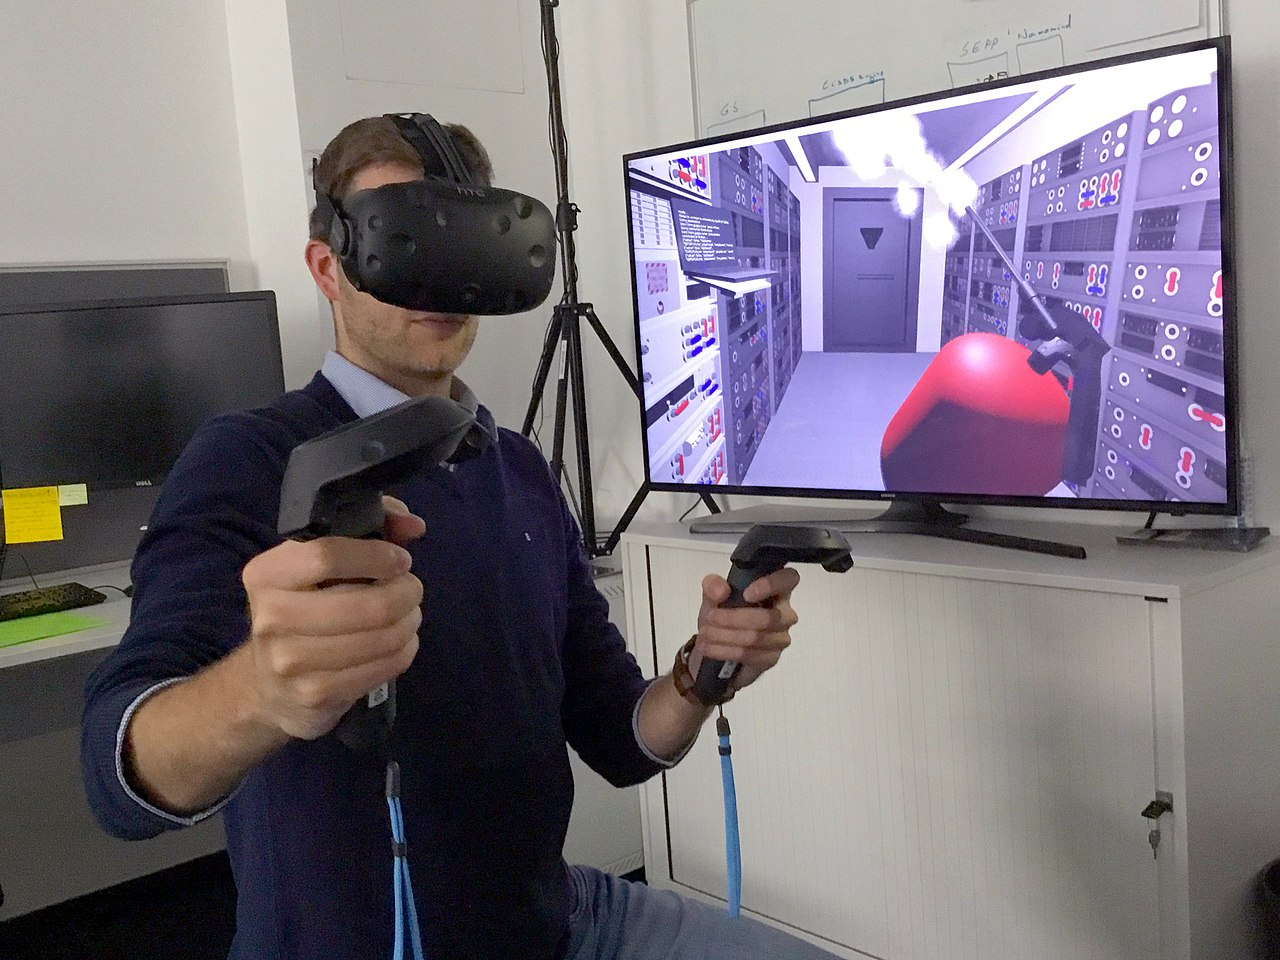
\includegraphics[width=0.5\linewidth]{images/vive.jpg}
	\caption{Ein Nutzer trägt das HMD der HTC Vive und bedient dessen Controller.}
	\label{img:vive}
\end{figure}

  
Im Folgenden sind Hersteller von VR-Systemen aufgelistet, sowie die Modelle, die derzeit auf dem Markt zum freien Verkauf stehen.

% REDO?
\begin{itemize}
\item Facebook (Oculus Rift und Oculus Go)
\item Google (Google Cardboard, Google Daydream)
\item HTC \& Valve (HTC Vive)
\item Microsoft (Microsoft HoloLens, Windows Mixed Reality)
\item Razer (OSVR Hacker Dev Kit)
\item Samsung (Samsung Gear VR)
\item Sony Computer Entertainment (PS VR)
\item Starbreeze Studios (StarVR)
\item Lenovo (Lenovo Explorer für Windows Mixed Reality und Lenovo Mirage Solo für Google Daydream)
\end{itemize}

//TODO:
Durchegehen
Vergleich der Hardware Vorteile, nachteile

TODO: 
HTC Vive und Vive PRo -> MR
%-------------------------------------------------------------
\section{Verarbeitung von MRT-Daten}						 %
%-------------------------------------------------------------
Obwohl die Darstellung von MRT-Bildern in direktem Zusammenhang mit ihrem Zweck steht, bleibt die Verarbeitung der Daten auch bei verschiedenen Darstellungsformen gleich. 

\subsection{Arbeit eines Neurologen}
Wie bereits in Kapitel \ref{motivation} oberflächlich erläutert wurde, besteht der Nutzen eines MRTs darin, dass der behandelnde Arzt einen Einblick in die betreffenden Organe (hier das Gehirn) erhält. Dazu studiert er die einzelnen Schichten des Gehirns und hält Ausschau nach Anomalien.

Im Fall von Schlaganfällen sind diese ...

Wurde eine entsprechender Bereich identifiziert, markiert der Arzt diesen auf jeder einzelnen Schicht. 
\subsubsection{Schlaganfälle auf einem MRT}

Laut der \citet{schlaganfall} bezeichnet ein Schlaganfall eine plötzlich auftretende Störung der Gehirnfunktionen durch eine mangelhafte Durchblutung von Gehirnpartien. Die Nerven im Gehirn werden dabei nicht mit genügend Sauerstoff versorgt, was irgendwann zu Beschädigungen des Gehirns führen kann.

Die Diagnose eines Schlaganfalls erfolgt durch bildgebende Verfahren, wie MRT- oder CT-Scans. Anhand der Bilder kann ein Neurologe erkennen, um welche Art von Schlaganfall es sich handelt und ob dieser durch eine Hirnblutung oder einen Gefäßverschluss ausgelöst wurde. 

Die Besonderheiten in der Untersuchung von CT- und MRT-Bildern wird von \citet{schlaganfallBilder} beschrieben.
Oft wird dabei zuerst ein CT-Scan durchgeführt, da dieser schneller Ergebnisse liefert und meist verfügbarer ist, auch wenn die Qualität der Ergebnisse geringer ist als bei einem MRT. 
Auf einem CT können anhand der Form und Struktur des Gehirns Schwellungen entdeckt werden, die von einer Gefäßverstopfung herrühren können. Besonders gut auf CT-Bildern zu erkennen sind Hirnblutungen, da das austretende Blut als heller Bereich auf den Bildern dargestellt wird. 

Ein MRT liefert nicht nur genauere Bilder sondern kann unzureichend durchblutete Bereiche früher nach dem Eintreten der Schlaganfallsymptome verlässlich sichtbar machen, als es bei einem CT der Fall ist.
Der minderdurchblutete Bereich des Gehirns wird auf MRT-Bildern heller dargestellt als der Rest des Gewebes. Er wird von Neurologen markiert, um die Ausmaße und Lage des Schadens zu bestimmen und soll in mARt zusammen mit den MRT-Daten angezeigt werden können.

Nach der Diagnose wird versucht, das Blutgerinnsel durch Verabreichung von Medikamenten aufzulösen oder es mechanisch zu entfernen. Bei einer Hirnblutung kann ein operativer Eingriff nötig sein.
(Vgl. \citet{schlaganfallBehandlung})

\subsection{Software in der Radiologie}
\label{radiologieSoftware}
% https://www.dicomlibrary.com/meddream/md5/index.html?study=1.2.826.0.1.3680043.8.1055.1.20111102150758591.92402465.76095170
%Use Cases
%Bsp
Um eine Diagnose stellen zu können muss der Arzt die MRT-Bilder eines Patieten genau studieren. Diese Untersuchung der Daten wird digital durchgeführt. Um dem Arzt einen Einblick in den Datensatz zu geben, gibt es spezielle Anzeigeprogramme, die diesen darstellen kann und weiterhin relevante Funktionen bietet. 
  
Wie bereits beschrieben, liegen die MRT-Bilder meist im DICOM oder NIfTI Datenformat vor. Um die Dateien öffnen zu können, bedarf es deshalb bestimmter Software. Es stehen viele verschiedene Programme zur Darstellung von MRT-Bildern zur Verfügung. Und die Auswahl eines Programms hängt meist an der persönlichen Präferenz des Arztes. 
In Krankenhäusern besteht allerding in der Regel die Situation, dass die Bilder in einem Picture Archiving and Communication System (PACS) gespeichert. (Fußnote?) Dabei handelt es sich um einen Server, der unter anderem medizinische Bilddaten zentral speichert. Die Bilder werden von bildgebenden Verfahren aus z.B. der Radiologie direkt im PACS gespeichert. Von dort aus kann entweder mit speziellen Arbeitsplatzrechnern oder auch mit herkömmlichen Computern über den Browser auch die Bilder zugegriffen werden. Dies geschieht dann meistens durch einen entsprechenden Viewer, der in das PACS integriert ist. Die Speicherung und Verteilung von medizinischen Bilddaten ist oft durch den DICOM-Standart geregelt, der im Abschnitt \ref{datenformate} genauer beschrieben ist.

Die meisten Viewer Programme für MRT-Bilder, unabhängig davon, ob es sich um PACS-Viewer handelt oder nicht ähneln sich stark in den Funktionen die sie anbieten und ihrem Aufbau.

Meist können in mehreren Fenstern verschiedene Ansichten des gleichen oder unterschiedlicher Datensätze geöffnet werden. Jedes Fenster stellt dabei eine Sichtebene dar, die gleichzeitig den Querschnitt durch das Gehirn bildet. Die verschiedenen Sichtebenen können in den anderen Ansichten farblich kodiert eingezeichnet werden, damit der Arzt ein besseres Bild davon bekommt, welchen Teil des Gehirns er gerade betrachtet.
Klassischer Weise werden drei verschiedene Blickwinkel dargestellt, die an den X-, Y- und Z-Achsen ausgerichtet sind. Die Sichtebenen verlaufen dabei orthogonal zur Blickachse. Die Ebenen können entlang der Achsen verschoben werden. Auf diese Weise scrollt der Neurologe durch die verschiedenen Schichten des Gehirns. 
Bei den drei Ebenen handelt es sich um die Frontal- oder Coronalebene, die das Gehirn in vorne und hinten teilt, die Sagittalebene, die zwischen links und rechts verläuft und die Transversalebene, die eine Teilung zwischen oben und unten bewirkt.  
Bei dieser Zusammensetzung von Ebenen wird manchmal noch eine vierte Ansicht ergänzt, auf der entweder die Sagittalebene von der anderen Seite abgebildet ist oder durch das Ineinanderschieben der gerade angezeigten Schichten eine annähernd dreidimensionale Darstellung simuliert wird. 
In Abbildung \ref{img:mrtSoftware} ist die Oberfläche der XY-Viewers zu sehen, die beispielhaft die Ansichten zeigt.

Die Benutzeroberfläche bietet auch einige Interaktionen. Die wichtigsten sind dabei die, die es dem Arzt ermöglichen ein möglichst eindeutiges Verständnis vom Inneren des Gehirns zu erhalten.  Dazu zählen:

\begin{description}
\item [Scrollen durch die einzelnen Bildschichten]\hfill \\
Dies geschieht in der Regel durch die Auswahl einer der Ansichten und die Betätigung des Mausrads. 
\item [Einstellen von Kontrast und Helligkeit D]\hfill \\
adurch können schlecht sichtbare Strukturen erkennbarer gemacht werden. Das Werkzeug dazu muss in der Taskleiste ausgewählt werden. In einem separaten Fenster können die Werte dann angepasst werden. ??
\item [Heranzoomen]\hfill \\
Bestimmte Bereiche eines Bildes können vergrößert werden, um sie besser beurteilen zu können.
\item [Verschieben des Bildausschnitts]\hfill \\
Um über ein vergrößertes Bild zu navigieren, kann der Nutzer dieses anklicken und in eine Richtung ziehen. Dies ermöglicht es andere Bildteile zu untersuchen, ohne zuerst herauszoomen zu müssen.
\end{description}

Obwohl über die Taskleiste oft noch weitere Optionen zur Verfügung stehen sind diese nicht essenziell zur Untersuchung der Bilder und werden meistens nicht oder nur in geringem Umfang genutzt, wie aus den Interviews mit Neurologen hervorging.

Es gitb eine Vielzahl von Viewern dieser Art zum Öffnen oder zur Verarbeitung von MRT-Bildern, viele davon stehen kostenloas im Internet zur Verfügung. 
Zu den wahrscheinlich meist verbreitetsten gehören \textit{Osirix} von \citet{osirix} und \textit{Horos} von \citet{horos}, für das Betriebsystem macOS. \citet{radiocafe} stellt außerdem folgende Viewer zum Gebrauch im radiologischen Kontext für Windows vor: Das kompakte und schnelle Viewerprogramm \textit{RadiAnt} von \citet{radiant}. Weiterhin \textit{Stratovan Pro Surgical 3D} von \citet{prosurgical}, was sich eigentlich an Chirurgen richtet und \textit{Navegatium DICOM Viewer}von \citet{navegatium}, ein Programm, dass auch als Windows App und somit auch für Tabletts zur Verfügung steht.
Alle der genannten Viewer besitzen die Funktion aus MRT-Datensätzen auch Volumendarstellungen zu erzeugen.

%-------------------------------------------------------------
\section{Interaktion in AR/VR}	
\label{VRInteraktion}							 %
%-------------------------------------------------------------
\subsection{Systeminterne Nutzereingaben}

VR- und AR-Systeme, die es heutzutage zu kaufen gibt besitzen in der Regel  eine oder mehrere Formen der Eingabe, um mit dem System zu interagieren. Da mARt als AR-Anwendung konzipiert ist, werden die verschiedenen Mittel zur Eingabe an dieser Stelle vorgestellt.

Die Eingabemöglichkeiten sind dabei teilweise von der Art des Systems abhängig. 
Beispielsweise kann für Smartphone-Apps der Touchbildschirm des Gerätes für die Nutzereingabe genutzt werden. 

Theoretisch kann jedes System mit jedem Eingabemediun verknüpft werden. Dies ist allerdings für Nutzer und Entwickler mit entsprechendem Aufwand verbunden. Die Techniken, die von den derzeit erhältlichen AR und VR Systemen verwendet werden, um Nutzereingaben zu erfassen lassen sich in zwei Kategorien teilen. 
%IMMERSION
\paragraph{Controller}
Zum einen gibt es Controller, die mit dem System zusammen hergestellt werden und die der Nutzer während der Verwendung des Systems in der Hand hält. Im Fall von VR Systemen sind meistens zwei Controller vorhanden, einer für jede Hand. Diese sind jeweils mit einer Anzahl an Knöpfen oder auch Touchpads versehen, die des Nutzer bedienen kann. Im Aussehen sind sich Controller dieser Art recht ähnlich. In Abbildung \ref{img:VRController} ist der Controller des HTC Vive Systems zusehen.
Allerdings existieren auch Systeme für dessen Bedienung nur ein Controller vorgesehen ist. Ein VR-Beispiel ist die \textit{Oculu Go}, ein eigenständiges System für grafisch weniger anspruchsvolle Anwendungen. 
Auch AR-Systeme, wie die \textit{Magic Leap} oder die \textit{Hololens} besitzen nur einen Controller. Diese haben im Vergleich zu den zuerst genannten VR-Controllern deutlich weniger Eingabemöglichkeiten. Im Falle der \textit{Hololens} handelt es sich um einen flachen Kontroller, den sich der Nutzer an den Finger steckt. Indem er Druck ausübt, kann er klicken. Daneben wird nur die Position und Rotation des Clickers verfolgt, durch die der Nutzer mit dem System interagieren kann. Das Gerät stellt damit eine von zwei möglichen Eingabemethoden dar. 

\paragraph{Gesten}
Die andere ist die Steuerung über Gesten, die vor allem AR-Systeme verwenden und die zweite Kategorie darstellt.
Die in den Systemen verbaute Kamera erfasst dabei die Hände des Nutzers in ihrem Blickfeld und erkennt bestimmte Handgesten, auf die dann reagiert wird. 
Die \textit{Hololens} kann zum aktuellen Zeitpunkt zwei Hauptgesten erkennen, \textit{Boolm} und \textit{Air tap}, sowie die Bewegung der Hand. Durch die Verbindung von beidem können beispielsweise Objekte verschoben werden. In Abbildung \ref{img:hololensGestures} ist dargestellt, wie die Hololens-Gesten ausgeführt werden. 
Die derzeit angekündigte \textit{Hololens 2} verfügt dagegen über eine Hand-Tracking-Funktionalität, die jede Bewegung der Hände, wie z.B. das Greifen von Objekten erkennt (vgl. \citet{hololens2}). 

Die \textit{Magic Leap} erkennt dagegen acht verschiedene Handgesten, die in \ref{img:magicGestures} abgebildet sind. 


\begin{figure}
	\centering
	%https://www.researchgate.net/figure/The-common-air-tap-gesture-used-in-the-HoloLens-application_fig2_32914899
	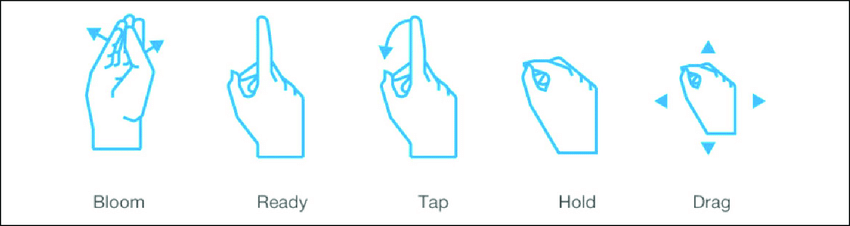
\includegraphics[width=0.7\linewidth]{images/hololensGestures.png}
	\caption{Handgesten, die die Hololens erkennt.}
	\label{img:hololensGestures}
\end{figure}

\begin{figure}
	\centering
	%https://next.reality.news/news/new-magic-leap-gesture-documentation-offers-insight-into-hands-will-make-its-digital-world-come-alive-0183614/
	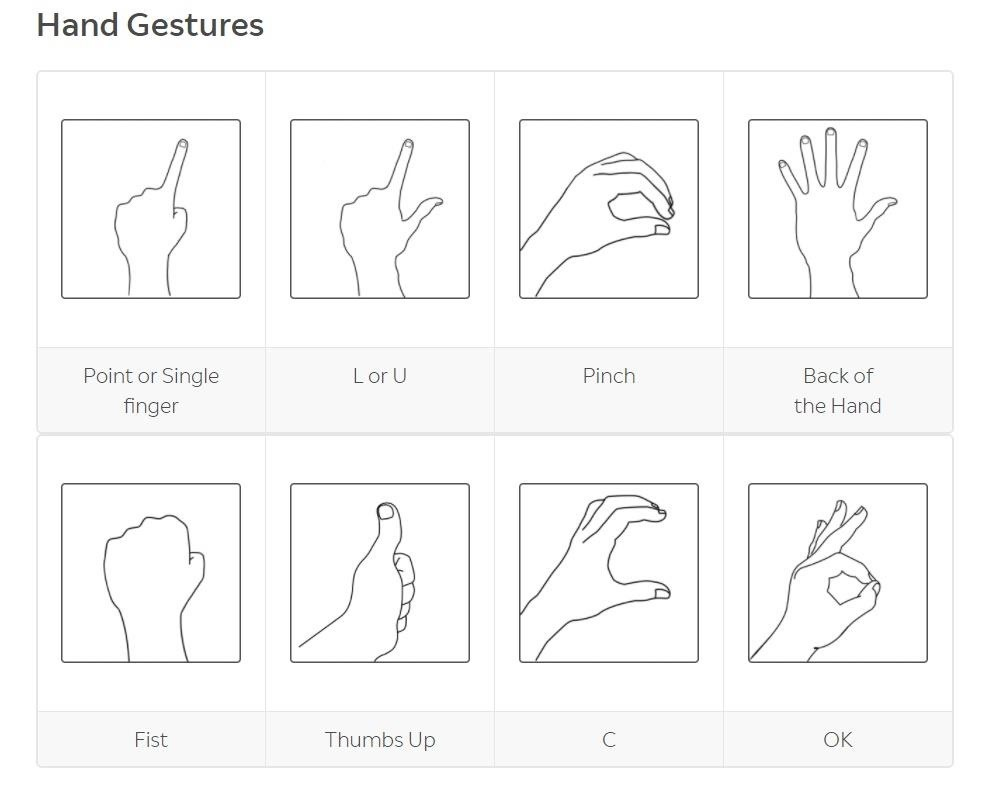
\includegraphics[width=0.7\linewidth]{images/magicleapGestures.jpg}
	\caption{Handgesten, die die Magic Leap erkennt.}
	\label{img:magicGestures}
\end{figure}

\paragraph{Kopfposition und Blickrichtung}

\paragraph{Sprachsteuerung}
\paragraph{HMD-Knöpfe}
Schließlich besitzen in vielen Fällen auch die HMDs der Systeme Knöpfe oder Räder. Diese dienen allerdings meistens zur Konfiguration des Systems und Steuern z.B. die Lautstärke.
%Linsenabstand? Capture?

Controller
\subsection{Leap Motion}

Die \textit{Leap Motion} von \citet{leapMotion} ist ein externes Gerät, dass die Hände des Nutzers tracked und die genauen Handbewegungen an einen Computer übermitteln kann. 
Um die Informationen zu sammeln, ist die \textit{Leap Motion} mit drei Infrarotemittern und zwei Kameras ausgestattet (vgl. \citet{Weichert13}). Das Gerät wird über USB an einen Rechner angeschlossen und kann dann als unabhängiges Eingabemedium verwendet werden. Allerdings ist auch eine Verwendung in Kombination mit AR- oder VR-Systemen möglich. 
Die \textit{Leap Motion} schafft es die Handbewegungen des Nutzers verlässlich nachzuempfinden, sodass die Hände in den digitalen Raum übertragen werden können. Hier kann nun eine Interaktion mit anderen digitalen Objekten stattfinden. 

Wie in Kaptel \ref{konzept} erläutert wird, wird die die \textit{Leap Motion} mit einem HMD kombiniert, um dem Nutzer die Möglichkeit zu geben mARt mit seinen Händen zu steuern.

\subsection{Andere}
Consolen Controller
\subsection{Interaktionsdesign}

//TODO:
Paper zur interaktion finden
-> was ist gut zur interaktion inAR warum?

\section{AR und VR im Vergleich}

Nachdem die AR- und VR-Systeme vorgestellt wurden, sollen die beiden Technologien an dieser Stelle verglichen werden.

\begin{tabular}{lrr} 
\toprule
Vergleich AR und VR\\  
\midrule 
Technologie & Vorteile & Nachteile\\ 
\midrule 
AR & Unabhängig von anderen Geräten & Eingeschränkte Interaktionsmöglichkeiten\\
   & Bewegungsfreiheit				& Entwicklung an Hersteller gebunden\\
   & Be								& Begrenzte Leisutung\\
   & Interaktion mit Umwelt möglich & Langes Tragen unkomfortabel\\
   & 								& Eingeschränktes augmentiertes Sichtfeld\\
VR & Leistungfähigkeit nur durch Rechner beschränkt  & Totale Abkapselung von der Umwelt \\
	& Kann auch kabellos verwendet werden		  	 & Langes Tragen unkomfortabel\\
	& & \\
\bottomrule
\end{tabular}







% Anforderungsanalyse

\chapter{Anforderungsanalyse}
\label{anforderung}

\section{Interviews}

Wie bereits beschrieben, ist es das Ziel dieser Arbeit Neurologen eine dreidimensionale Darstellung von Gehirn-MRT-Scans in einer interaktiven AR- bzw. VR-Anwendung zur Verfügung zu stellen, um zu untersuchen, inwiefern diese die Ärzte in ihrer Arbeit besser unterstützt, als bisher verwendete Darstellungssoftware. Die hypothetischen Vorteile eines solchen Programmes wurden im Kapitel \ref{motivation} erläutert.
Für den Vergleich mit bisheriger Software ist eine Anwendung prototypischen Charakters ausreichend. Diese soll auf die grundlegenden Interaktionen beschränkt sein, die ein Neurologe für die Verarbeitung der Daten benötigt.

Der Fokus der Untersuchung liegt auf dem Bereich der akuten Schlaganfallbehandlung. Wie im Kapitel \ref{grundlagen} beschrieben untersucht der Neurologe hierfür die Abbildungen des Gehirns eines Patienten, die durch den MRT-Scan erzeugt wurden. Dabei hält er nach Bereichen Ausschau, die von einem Schlaganfall betroffen sein könnten, um die Art des Schlaganfalls zu bestimmen, ? sowie den entstandenen Schaden einschätzen zu können. Betroffene Bereiche werden anschließend vom Arzt markiert. Diese Markierung kann danach ein- und ausgeblendet werden.

Um zu bestimmen, welche Interaktionen und Funktionen ein Neurologe benötigt, um effektiv mit der Anwendung arbeiten zu können, wurden iterativ mehrere Interviews mit dem betreuenden Neurologen der Charité Berlin geführt. Die Antworten des Arztes wurden in Anforderungen übertragen, die im folgenden Abschnitt festgehalten wurden. 

\section{Anforderungen als User Stories}

Die im Gespräch mit dem Arzt entwickelten Anforderungen an mARt wurden in Tabelle \ref{tab:userStories} als User Stories.
User Stories werden in der Software-Entwicklung verwendet, um einzelne Funktionen zu definieren, die möglichst unabhängig voneinander implementiert werden können sowie mehr aus Sicht des Nutzers zu denken, statt aus der Sicht des Entwicklers (\cite{UserStoriesApplied)}.
Zur besseren Referenzierung wurden die Stories jeweils mit Bezeichnern versehen. Da viel der Interaktionen sowohl für die zwei- als auch dreidimensionale Darstellung benötigt werden wurde weiterhin gekennzeichnet, welche Darstellung von der jeweiligen Story betroffen ist.

\begin{longtable} {p{.125\textwidth}p{.50\textwidth}p{.05\textwidth}p{.225\textwidth}}
\toprule
Bezeichnung & User Story & 2D/3D & Anforderungsreferenz \\
\toprule
U01 & Als Nutzer möchte ich eine möglichst genaue und gut erkennbare Abbildung der MRT-Bilder, damit ich eine Vorstellung habe, wie das Gehirn des Patienten aussieht. & beide & A05\\
\midrule 
U02 & Als Nutzer möchte ich die Daten als zweidimensionale Schichten aus mindestens einem Winkel betrachten können, um diese wie gewohnt untersuchen zu können.  & 2D & A02\\
\midrule 
U03 & Als Nutzer möchte ich die Daten als dreidimensionales Volumen betrachten können, um ein besseres Verständnis für den Zustand des Gehirns zu erhalten. & 3D & A02\\
\midrule 
U04 & Als Nutzer möchte ich mindestens zwei Datensätze nebeneinander anzeigen lassen, um direkte Vergleiche zwischen diesen ziehen zu können. & beide & A14\\
\midrule 
U05 & Als Nutzer möchte ich aus verschiedenen Datensätzen auswählen können, welche angezeigt werden, um mich auf die relevanten Daten konzentrieren zu können. & beide & A01\\
\midrule
U06 & Als Nutzer möchte ich entscheiden können, ob ich mehrere angezeigte Datensätze gleichzeitig oder einzeln manipuliere (z.B. Kontrast), um die Einstellungen genau an jeden Datensatz anpassen zu können. & beide & A14\\
\midrule 
U07 & Als Nutzer möchte ich auf mindestens einer Achse durch beide Darstellungen scrollen können, um das Innere des Organs zu untersuchen. & beide & A04\\
\midrule 
U08 & Als Nutzer möchte ich mit einem Scrollrad durch die Darstellungen scrollen können, um genaue Kontrolle darüber zu haben, welche Schichten angezeigt werden. & beide & A11\\
\midrule 
U09 & Als Nutzer möchte ich zwischen einer zwei- und dreidimensionalen Darstellung der Daten wechseln können, um die Vorteile beider Darstellungen für meine Untersuchung zu nutzen. & beide & A02\\
\midrule 
U10 & Als Nutzer möchte ich, dass bisherige Manipulationen beim Wechsel zwischen 2D und 3D übernommen werden, um die Orientierung und Sichtbarkeit zu erhalten. & beide & A13\\
\midrule 
U11  & Als Nutzer möchte ich den gekennzeichneten vom Schlaganfall betroffenen Bereich ein- und ausblenden können, um mich auf diesen, oder die Darstellung an sich konzentrieren zu können. & beide & A02\\
\midrule
U12 & Als Nutzer möchte ich auch dann noch die Strukturen des Gehirns erkennen, wenn der gekennzeichnete Bereich eingeblendet ist. & beide & A03\\
\midrule 
U13 & Als Nutzer möchte ich die MRT-Darstellungen drehen können, um den besten Blickwinkel auf den für mich relevanten Bereich zu bekommen. & 3D & A09\\
\midrule 
U14 & Als Nutzer möchte ich die Helligkeit und den Kontrast der Darstellung verändern können, um Strukturen besser deutlich zu machen. & beide & A09\\
\midrule 
U15 & Als Nutzer möchte ich die MRT-Darstellungen skalieren können, um die Darstellung gut zu erkennen. & beide & A08\\
\midrule 
U16 & Als Nutzer möchte ich die MRT-Darstellungen frei im Raum bewegen können, um sie meiner Position anzupassen. & beide & A07\\
\midrule 
U17 & Als Nutzer möchte ich, dass das Hologram seine Position im Raum behält, um es von allen Seiten betrachten zu können. & beide & A13\\
\midrule 
U18 & Als Nutzer möchte ich alle vorhandenen MRT-Sequenzen sehen und zwischen ihnen wählen können, damit ich alle notwendigen Informationen zu dem Scan nutzen kann. & beide & A12\\
\midrule 
U19 & Als Nutzer möchte ich Dateien im NIfTI-Format in der Anwendung verwenden können, damit ich sie nicht vorher umwandeln muss. & beide & A13\\
\midrule 
U20 & Als Nutzer möchte ich Dateien im DICOM-Format in der Anwendung verwenden können, damit ich sie nicht vorher umwandeln muss. & beide & A13\\

\bottomrule
\caption{\label{tab:userStories}Aus Interviews abgeleitete User Stories.}
\end{longtable}


% Konzept

\chapter{Konzept}
\label{konzept}

Im folgenden werden Konzepte diskutiert, um die in Kapitel \ref{anforderung} herausgearbeiteten Anforderungen zu erfüllen.

\section{Implementierungsziele}
Ziel des Arbeit ist es eine prototypische AR- bzw. VR-Anwendung zur Visualisierung und Untersuchung von MRT-Daten zu implementieren. 

Vor allem im Bereich der Volumendarstellung gibt es bereits viele Programme und Arbeiten, die diese erfolgreich umsetzten, wie im Kapitel \ref{grundlagen} erläutert wurde.
Wie später beschrieben wird, baut mARt auf einer bereits implementierten Lösung auf. Die Anwendung soll mit der Spiele-Engine \textit{Unity}  implementiert werden, worauf ebenfalls im späteren Kapiteln eingegangen wird. Die Implementierung muss also mit der Software kompatibel sein. In Kapitel \ref{grundlagen} wurde unter anderem die \textit{Unity}-Erweiterung \textit{Volume Viewer Pro} beschrieben, die viele der gestellten Anforderungen bereits abdeckt. Das Programm ist allerdings kostenpflichtig. Eine unabhängige und frei zugängliche Software ist dem vorzuziehen. Vor allem, da es sich um einen Prototyp handelt, der Aufschluss über die Verwendungsmöglichkeiten in diesem Bereich liefern und daher eventuell weiterentwickelt werden soll. Deshalb sollte die dreidimensionale Darstellung im Rahmen dieser Arbeit entwickelt werden und Code aus anderen Quellen nur verwendet werden, wenn er diesen Kriterien (z.B. lizenzrechtlichen Bestimmungen) entspricht.

Weiterhin soll die Darstellung in eine interaktive Anwendung eingebettet sein, die die in Kapitel \ref{anforderung} formulierten Anforderungen erfüllt.

\section{3D Darstellung}
\label{3dDarstellung}

Im Kapitel\ref{grundlagen} wurden verschiedene Methoden vorgestellt, um ein Volumen zu visualisieren. An dieser Stelle soll diskutiert werden, welche davon sich am besten für die Umsetzung in mARt eignet.
Die 3D-Darstellung sollte die in Kapitel \ref{anforderung} beschriebenen Eigenschaften haben:

\begin{itemize}
\item Darstellung sollte das Volumen dreidimensional abbilden. \textbf{(U03)}
\item Die innere Struktur des Gehirns sollte erkennbar sein \textbf{(U01)}
\item Die Markierung des vom Schlaganfall betroffenes Bereichs sollte die MRT-Darstellung nicht unkenntlich machen. \textbf{(U12)}
\item Es sollte möglich sein durch die Schichten des Volumes zu scrollen. \textbf{(U07)}
\end{itemize}

Dadurch lassen sich Aussagen über das gewünschte Aussehen der Darstellung herleiten.
Da das Innere der 3D Darstellung erkennbar sein soll, muss eine semi-transparente Darstellung erzeugt werden, die sowohl die Form des Gehirns abbildet, als auch die innere Struktur. Die eingeblendete Markierung sollte ebenfalls zu einen gewissen Grad transparent sein.
Weiterhin sind sind nur die Pixel relevant, die das Gehirn darstellen. Der Bereich darum (Schädel und Hintergrund) sollten gefiltert  und nicht sichtbar gemacht werden. Das gewünschte Ergebnis ist, dass das Gehirn frei im Raum schwebt. 

Die Anforderungen sprechen gegen eine Umsetzung, die eine Oberfläche des Gehirns erzeugt und es als Mesh darstellt. Die Form des Gehirns könnte dadurch deutlich gezeigt werden und das Objekt würde von den umgebenden Pixeln getrennt werden. 
Allerdings handelt es sich bei dem Gehirn nicht um eine Hülle sondern eine Masse. Es ist unwahrscheinlich, dass ein Verfahren wie Marching Cubes die inneren Gehirnstrukturen exakt genug wiedergeben könnte, damit ein Neurologe sinnvolle Schlüsse daraus ziehen kann. Die binäre Aufteilung der Voxel kann außerdem dazu führen, dass Teile des Gehirn fehlerhafter Weise nicht angezeigt werden. Weiterhin müsste das Mesh in Echtzeit kontinuierlich angepasst werden, wenn der Nutzer durch die verschiedenen Schichten scrollt. 
Deshalb eignet sich eine Oberflächengenerierung nicht zur Visualisierung.
Hinzu kommt, dass in den Anforderungen kein Anwendungsfall beschrieben wird, der eine Oberfläche erfordert, wie z.B. die Berechnung einer Kollision des Gehirns mit einem anderen Objekt.	
	
Die dreidimensionale Darstellung lässt sich demnach besser mit einer Volume Rendering Methode umsetzten.  
In Kapitel \ref{grundlagen} wurden die verschiedenen Volume Rendering Techniken miteinander verglichen.
Die Visualisierung der MRT-Daten wurde im Rahmen dieser Arbeit mit den Volume Raycasting Verfahren umgesetzt.
Das Raycasting Verfahren liefert die beste Bildqualität, wie aus dem Vergleich hervorgeht. Es ist daher auch weit verbreitet bei der Implementierung von Volume Rendering Software, wie in Abschnitt \ref{volumeRenderingImplementierung} gezeigt wurde. 
Die verschiedenen Implementierungen können zur Orientierung und als Referenz für die eigene Umsetzung verwendet werden.
Die Technik lässt sich außerdem gut durch einen Fragment-Shader realisieren was eine Implementierung in \textit{Unity} erleichtert. 
Das für Texture-Based Rendering benötigte Texture Slicing und Mapping ist in der Umsetzung nicht trivial und die Ergebnisse des Verfahrens rechtfertigen diesen Aufwand nicht.
Obwohl die Shear-Warp Methode in der Theorie ähnlich abläuft wie das Raycasting, ist die Implementierung komplexer.
Für eine Umsetzung des Volume Renderings im Rahmen dieser Arbeit eignet sich das Raycasting Verfahren deshalb am besten.
Zwar ist die Berechnung einzelner Strahlen leistungsintensiv, kann aber durch Optimierungen und die Verwendung von passender Hardware trotzdem in Echtzeit und interaktiv realisiert werden.

Weiterhin wurden in Abschnitt \ref{klassifikation} die verschiedene Arten erläutert eine Klassifikation zu implementieren. Durch die Umsetzung im Fragment-Shader wird eine Post-Klassifikation umgesetzt. 
Von der Umsetzung einer Pre-Integrierten Klassifikation wurde abgesehen. Zum Einen auf Grund des zusätzliche Implementierungsaufwands, zum Anderen weil die Renderings keine schwerwiegenden Artefakte aufwiesen. Letzteres wird im Abschnitt \ref{ergebnisse} aufgegriffen.

Wie im Kapitel \ref{grundlagen} beschrieben, werden beim Volume Rendering in der Regel Transferfunktionen eingesetzt, um verschiedene Gewebestrukturen oder Materialien zu unterscheiden. Dabei handelt es sich um eine Look-Up-Tabelle in Form einer Textur, die jedem Isowert eine Farbe und Opazität zuweist.
Die Herausforderung bei der Implementierung einer Transferfunktion ist dabei die Generierung einer zum Datensatz passenden Textur. Selbst bei einer Transferfunktion mit nur einer Dimension müssen häufig verschiedene Wertzuweisungen ausprobiert werden, um ein gutes Ergebnis zu erhalten.
Um eine bzw. mehrere Transferfunktionen zu generieren, die den Ansprüchen des Nutzers genügt und die für verschiedene Datensätze passend sind, ist es deshalb sinnvoll dem Nutzer eine Benutzeroberfläche zur Verfügung zu stellen, mit deren Hilfe er die verwendete Transferfunktion zur Laufzeit manipulieren kann. 

In einem Volumen gibt es in der Regel bestimmte Isowerte, die Grenzwerte zwischen verschiedenen Materialien darstellen. Diese dienen als Kontrollpunkte zwischen denen interpoliert wird, um einen Farbverlauf zwischen den Materialien zu erhalten. 
Um die Transfertextur zu beeinflussen muss der Nutzer diese Kontrollpunkte verändern können. Er muss dabei für jeden Kontrollpunkt dessen Iso-, Farb- und Opazitätswert festlegen. Zwischen den Werten der Kontrollpunkte kann dann eine Spline-Interpolation stattfinden.
Die nutzergesteuerte Generierung von Transferfunktionen konnte aus zeitlichen Gründen im Rahmen dieser Arbeit nicht umgesetzt werden.


\section{Darstellung des gekennzeichneten Bereichs}
\label{maske}


In User Story \textbf{U11} der Anforderungen wird beschrieben, dass der vom Schlaganfall betroffene Bereich des Gehirns, der vorher von einem Arzt gekennzeichnet wurde in der Darstellung angezeigt werden soll, wenn dies gewünscht wird. 
Der Bereich wird durch Masken definiert, die zuvor von einem Arzt in einem externen Programm erstellt wurden und ebenfalls im NIfTI-Format vorliegen. Für jede Schicht in einem Datensatz existiert ebenfalls eine Schicht im Maskendatensatz. 

Der Bereich soll sowohl in der zwei- als auch in der dreidimensionalen Ansicht dargestellt werden. Bei letzterer sollte er auch in den Querschnitten erkennbar sein, die sich durch das Scrollen durch das Volumen ergeben. MRT-Daten und markierter Bereich verhalten sich also gleich.

Da die Daten im selben Format vorliegen und sich gleich verhalten sollen, ist es naheliegend, dass sie auf die selbe Weise gerendert werden. Dementsprechend werden auch die Maskenbilder in eine 3D-Textur übertragen, die dann durch Volume Raytracing gerendert wird. Damit aber nicht jeder Strahl doppelt verschossen werden muss, der das Volumen durchdringt, wird der Zugriff auf die Maskentextur in den Shader integriert, der bereits das MRT-Volumen rendert. Für jeden Voxel, der aus der 3D-Textur der MRT-Daten gelesen wird, wird  der Voxel mit denselben Koordinaten aus der Masken-3D-Textur gelesen. Die zwei Farbwerte werden zum Schluss miteinander verrechnet. Durch die Verrechnung, bleibt trotzdem die Struktur des Gehirns erkennbar, wie es von \textbf{U12} gefordert wird. Die Abfrage der Maskenwerte erfolgt nur, wenn durch das Material eine entsprechende Steuervariable gesetzt wurde.
Dies wird im folgenden Codebeispiel veranschaulicht.

\begin{listing}[!htb]
\begin{minted}[mathescape,
               linenos,
               numbersep=5pt,
               gobble=2,
               frame=lines,
               framesep=2mm]{csharp}
void main(sampler3D _Volume,
		  sampler3D _MaskVolume,
          sampler1D _TransferTexture,
          float3 texCoord : TEXCOORD0,
          float4 maskColor : COLOR,
          float _ShowMask)
          {
          
          	// Isowert des Volumens wird für die aktuelle Position ausgelesen
          	float isoValue = tex3D(_Volume, texCoord);
          
          	if (_ShowMask == 1)
          	{
          		// Isowert des Maskenvolumens wird für die 
          		// aktuelle Position ausgelesen
          		float isoValueMask = tex3D(_MaskVolume, texCoord);
          	
          		// Die Maske wird eingefärbt
          		isoValueMask *= maskColor;
          	}
          
          	// Die Werte werden verrechnet
          	return isoValue * isoValueMask;
          }
\end{minted}
\caption{Bestimmung der Farbe eines Pixels in Abhängigkeit zum entsprechenden Isowert sowie dem Iso- und Farbwert der Maskentextur. Letztere werden nur angewandt, wenn die Steuervariable dafür gesetzt wurde. Selbst erstelltes Beispiel}
\label{lst:transfer}
\end{listing}
\FloatBarrier

\section{2D Darstellung}

Neben der dreidimensionalen Ansicht sollen die Daten auch in zwei Dimensionen untersucht werden können, wie es auch in vielen Bildschirmanwendungen der Fall ist.
Die Betrachtung von jeweils nur einer Schicht des Datensatzes erlaubt es den Fokus auf bestimmte Merkmale oder Regionen zu legen, die in dieser Darstellung deutlicher sein könnten als in der volumetrischen. Weiterhin wird der direkte Vergleich zwischen den Szenen deutlicher. Beispielsweise kann die Annahme von der Größe eines Bereichs in der 3D-Darstellung überprüft und so eventuell korrigiert werden.

Da in User Story \textbf{U02} nur das Scrollen auf einer Achse durch die Bildschichten gefordert wird, wird jeder Datensatz als quadratische Bildfläche dargestellt.
Die Anzeige der Daten aus verschiedenen Sichtachsen wäre nicht nur aufwändiger in der Umsetzung, sondern würde die Komplexität der Anwendung auch deutlich steigern, wodurch ihre Benutzbarkeit sinken könnte. 

Die zweidimensionale Darstellung in mARt kann kaum einen Mehrwert gegenüber einer Bildschirmanwendung  bieten. Zwar kann sie zur Untersuchung der Daten genutzt werden, dient allerdings hauptsächlich als komplementäre Ansicht zur 3D-Visualisierung.

\section{Endgerät}
\label{device}

Wie bereits im Abschnitt \ref{motivation} beschrieben, ist mARt als AR-HMD-Anwendung konzipiert. Obwohl die Technologie noch viele Unzulänglichkeiten aufweist, eignet sie sich auf lange Sicht dennoch besser für den Einsatz in einem medizinischen Arbeitsumfeld.
Für den Arbeitsalltag eines Arztes und die Zusammenarbeit mit Patienten eignet sich ein durchsichtiges Display deutlich besser als ein undurchsichtiges. Der Nutzer verliert somit nicht seine Umwelt aus den Augen, wodurch er sich sicherer in der Benutzung fühlt. In einem Anwendungsszenario, in dem er mit anderen Menschen kommuniziert, während er die Anwendung bedient, gilt dies umso mehr. Die mögliche Verwendung von mARt während einer Operation oder Behandlung wäre mit einer VR-Anwendung oder Smartphone-App unmöglich. Die Reduzierung auf die virtuelle Realität bietet zudem keinen Vorteil für die Funktion der Anwendung, da die Umwelt in der Anwendung nicht verändert werden soll. 

Ein weiterer Vorteil eines AR-HMDs ist seine Portabilität. Dies ist vor allem entscheidend, wenn die Daten anderen Personen, wie z.B. Patienten gezeigt werden sollen. Das Gerät lässt sich einfach in ein anderes Zimmer mitnehmen, was mit einem VR-System deutlich schwieriger umzusetzen ist.
 
Eine große Einschränkung bietet die geringe Anzahl an Gesten und Interaktionsmöglichkeiten, die die bisherige AR-Technik zur Verfügung stellt. Dies ist allerdings hinfällig, wenn stattdessen die \textit{Leap Motion} verwendet wird, um Nutzereingaben zu erfassen. Die Vorteile des Gerätes werden im folgenden Abschnitt erläutert.

Es ist zu erwarten, dass sich AR-HMDs in den folgenden Jahren deutlich verbessern werden, was Tragekomfort und Leistungfähigkeit angeht. Da mARt als Prototyp einer medizinischen Anwendung anzusehen ist, kann davon ausgegangen werden, dass bei einer Weiterentwicklung der Anwendung Technologie zur Verfügung steht, die viele der genannten Mängel behebt.

Eine AR-Anwendung eignet sich demnach besser für die Umsetzung. Um diese wiederzugeben wurde die \textit{HoloLens} von \cite{hololens} gewählt, da sie bereits 2015 erschienen und verfügbarer ist.
Die Leistung des Gerätes ist allerdings nicht ausreichend, um die intensiven Berechnungen durchzuführen, die für das Volume Raycasting erforderlich sind. Auch der Einsatz der \textit{Leap Motion} erfordert eine hohe Rechenleistung.
In einer Demo, in der das Volume Rendering auf der \textit{HoloLens} getestet wurde, wurde eine Framerate von 2-10 FPS gemessen, wobei die höhere Rate nur bei einer Darstellung mit kleiner Skalierung erreicht wird. \cite{fpsHololens} empfiehlt eine Framerate von 60 FPS, um die beste Erfahrung zu bieten.
Die Framerate ist nicht ausreichend, um eine angenehme und effektive Arbeitsweise zu ermöglichen. 
Hinzu kommt, dass der Einsatz der \textit{Leap Motion} es verhindert, dass die Anwendung für die \textit{HoloLens} bereitgestellt wird. Dies wird in Abschnitt \ref{kombination} erläutert. Die Anwendung wird deshalb lediglich an die \textit{HoloLens} übertragen, was allerdings eine Latenz mit sich bringt. 
Um im Test eine stabile Darstellung und Interaktion zur Verfügung stellen zu können, wurde die Anwendung zusätzlich als VR-Anwendung umgesetzt. Die Funktionalität bleibt dabei gleich. 
Durch Verwendung der \textit{Leap Motion} ist die Interaktion mit dem Modell in beiden Anwendungen identisch. 
Zur Wiedergabe der VR-Awendung wird die \textit{HTC Vive} verwendet.
% Bezug Hololens2?

\section{Interaktionsdesign} 

In diesem Abschnitt wird das Konzept der Interaktion innerhalb der Anwendung beschrieben. Dazu wird zunächst diskutiert, mit welcher Technik die Nutzereingabe erfasst werden soll. Dann wird auf die Gestaltung der Bedienelemente in der Anwendung eingegangen.

\subsection{Nutzereingabe}
%\todo{Referenzen?}

Wie bereits im vorherigen Abschnitt erwähnt, wird die \textit{Leap Motion} in Kombination mit dem jeweiligen HMD benutzt, um den Nutzer mit der Anwendung interagieren zu lassen. 
Die \textit{Leap Motion} verfolgt die Hände des Nutzers und stellt diese als 3D-Modelle innerhalb der Anwendung dar. Die Bewegungen der Hände werden dabei genau nachempfunden, sodass die Illusion entsteht die simulierten Hände wären die eigenen. 
Bereits \cite{Zimmerman86} haben die Hand als natürlichstes Mittel zur Manipulation von Objekten bezeichnet. Zudem haben \cite{Bianchi-Berthouze07} festgestellt, dass Körperbewegung in einer Anwendung zu einem höheren Einsatz in deren Umgang führt. Indem es die Hand in den virtuellen Raum überträgt, fördert die \textit{Leap Motion} den intuitiven Umgang mit der Anwendung enorm und ermöglicht damit ein positives Nutzungserlebnis. Weiterhin wird dadurch das erlernen komplexer Gesten oder die Verwendung von Controllern umgangen. Beides sind Hindernisse, die Nutzer, die mit der Technik nicht vertraut sind abschrecken könnten. 
Nachteilig ist, dass das Sichtfeld der Kamera begrenzt ist. Da diese vorne auf dem HMD angebracht ist, wird dieses noch weiter nach vorne verschoben. Damit seine Hände erkannt werden, muss der Nutzer sie deshalb in einiger Entfernung genau vor sein Gesicht halten. 
Dafür bietet die \textit{Leap Motion} mehr Freiheit in der Interaktion. Dies gilt besonders im Vergleich zu den Eingabemöglichkeiten der \textit{HoloLens}, 
deren Gestenerkennung stark begrenzt ist. Um alle notwendigen Manipulationen der Darstellungen abzudecken, müssten daher entweder deutlich mehr Bedienelemente eingebaut werden oder die Interaktion müsste zu großen Teilen auf Sprachsteuerung beruhen. 
Dies wurde durch Implementierung einer prototypischen \textit{HoloLens}-Anwendung bestätigt, die nur durch die \textit{HoloLens}-Gesten gesteuert werden kann. Sie ist im Kapitel \ref{implementierung} genauer beschrieben.
Ein auf Sprachsteuerung beruhendes Programm ist im Arbeitsalltag eher umständlich, vor allem wenn sich der Anwender im selben Raum wie andere Personen befindet. Zudem wirft es die Problematik der Mehrsprachigkeit auf. 
Allerdings wurde im Frühjahr 2019 ein Nachfolgemodell der \textit{HoloLens} angekündigt, das alle Handbewegungen des Nutzers verfolgt und somit auch Gesten wie Greifen erkennt. Dies wird noch einmal in Abschnitt \ref{hololens2Fazit} erläutert. Es zeigt, dass eine Steuerung durch die Hände des Nutzers nicht nur sinnvoll ist, sondern in der Zukunft auch durch ein HMD umgesetzt werden kann.

Da mARt schließlich in Form einer AR- und VR-Anwendung umgesetzt wird stellt sich weiterhin die Frage nach den Bedienmöglichkeiten in VR. Die Verwendung der \textit{Leap Motion} ermöglicht es hier einerseits, dass beide Anwendung durch dieselben Interaktionen bedient werden können. Andererseits bietet sie auch gegenüber der Steuerung durch Controller Vorteile. 
Wie bereits erwähnt, kann die Bedienung der Controller einen ungeübten Nutzer verwirren. Dazu kommt, dass es sich dabei um eigenständige, für die Anwendung notwendige Geräte handelt. Im Arbeitsalltag müsste immer sicher gestellt werden, dass sie nicht abhanden kommen und zu jedem Zeitpunkt aufgeladen sind. 
Hinzu kommt, dass die Controller zur Verwendung in der Hand gehalten werden müssen. Der Nutzer wird somit der Fähigkeit des Multitasking beraubt, wozu z.B. das Schreiben von Notizen während der Nutzung der Anwendung fällt. Auch die Verwendung von Controllern während einer OP ist ausgeschlossen.

%\todo{bezug zu interaktion in grundlagen?}
\subsection{Konzeption der Interaktionselemente}
% 2D 
% UX steht im Vordergrung -> begründen warum besser als vorher!

Im Kapitel \ref{anforderung} ist definiert, welche Interaktionen bzw. Funktionalitäten dem Nutzer zur Verfügung stehen sollten, damit er die Anwendung sinnvoll Nutzen kann. 
Wie vorhergehend beschrieben, wird die \textit{Leap Motion} eingesetzt, um dem Nutzer eine möglichst intuitive Interaktion mit der Anwendung zu ermöglichen. Die Eingabe erfolgt dabei hauptsächlich durch seine Hände, die er frei im virtuellen/augmentierten Raum bewegen und somit mit digitalen Eingabeelementen interagieren kann. 
Dazu stehen ihm einerseits physische Bedienelemente wie Knöpfe, Schieberegler oder Räder zur Verfügung, die virtuell simuliert werden, andererseits die Bewegung der Hände selbst, z.B. durch das Ausüben von Gesten.

Physische Bedienelemente haben den Vorteil, dass sie dem Nutzer bereits aus anderen Kontexten bekannt sind. Dieses Vorwissen erleichtert in Verbindung mit Icons oder Beschriftungen das Verständnis der Elemente. 
Dadurch wird eine Verwendung ohne hohen Lernaufwand oder das Merken von Gesten ermöglicht. 
Die Elemente laden außerdem dazu ein sie auszuprobieren, sodass der Nutzer ermutigt wird, mit der Anwendung zu interagieren und sich so mit dieser vertraut zu machen. 
Allerdings ist es schwierig das physische Feedback zu simulieren, das der Nutzer erwartet, da die Elemente der physischen Realität nachempfunden sind. Der Tastsinn des Nutzers kann durch die Anwendung nicht simuliert werden. Es können lediglich audiovisuelle Reize erzeugt werden. Da der Sehsinn allerdings von allen der dominanteste ist \cite{Azmandian16}, kann durch die Verwendung dieser Reize eine immersive Interaktion erreicht werden. 
Schließlich ist zu beachten, dass Interaktionselemente dieser Art Raum innerhalb der virtuellen Realität einnehmen. Dementsprechend ist es wichtig diese so anzuordnen und zu gestalten, dass der virtuelle Raum für den Nutzer übersichtlich bleibt. Hier muss auch ein Gleichgewicht zwischen der Reduzierung der Elemente in Größe und Komplexität, sowie der Bedienbarkeit gefunden werden. Ist ein Knopf beispielsweise zu klein, fällt es schwer diesen zu betätigen. 

Für die Verwendung physischer Bedienelemente spricht außerdem, dass die Komplexität der Interaktionen zu hoch ist, um nur durch Gesten abgedeckt werden zu können. Der intuitive Einsatz der Hände für simple Interaktionen, wie z.B. das Drehen eines Objektes durch Anfassen, ist dabei trotzdem einer abstrakteren Abbildung auf Bedienelemente vorzuziehen. Der Einsatz von einzelnen, eindeutigen Gesten ist weiterhin hilfreich, um der eben genannte visuellen Reizüberflutung entgegen zu wirken. 
Bei der Konzeption der Interaktion mit der Anwendung wird also zuerst angestrebt eine intuitive direkte Bedienmöglichkeit per Hand oder Geste zu verwenden und bei komplexeren Interaktionen möglichst einfach gestaltete physische Bedienelemente einzusetzen.
Im Folgenden wird erläutert, wie die in \ref{anforderung} beschriebenen Interaktionen innerhalb der Anwendung gestaltet wurden.

% Scrollen
Die zentrale Interaktion ist dabei das Scrollen durch die Bildschichten, beschrieben durch \textbf{U07}, die es dem Nutzer ermöglicht einen Einblick in das Innere des Gehirns zu erlangen. In Bildschirmanwendungen wird die Bewegung durch die Schichten meistens durch Betätigung des Scrollrads der Maus erreicht, wie in Kapitel \ref{grundlagen} erläutert wurde.
Dies erfordert geringen Aufwand, ermöglicht es dem Nutzer schnell die Richtung der Bewegung zu ändern und liefert außerdem oft haptisches Feedback. 
Aus diesem Grund ist in Anforderung \textbf{U08} die Verwendung eines Scrollrads zu diesem Zweck beschrieben. Durch die Verwendung der \textit{Leap Motion} entfallen allerdings andere Eingabemittel als die Hände des Nutzers.
Trotzdem sollte der Wechsel zwischen den Schichten in VR/AR möglichst genauso direkt und intuitiv sein. 
Hierzu bieten sich für die 2D- und 3D-Darstellungen verschiedene Möglichkeiten, weswegen die Bedienung sich für diesen Fall in den Szenarien unterscheidet. 

In beiden Darstellungen wird die aktuell angezeigte Schicht durch das Volumen bewegt. Bei einem Volumen lässt sich diese sehr verständlich als Ebene darstellen. Um dieses zu verschieben, ist die direkteste Aktion diese mit der Hand zu greifen und in eine Richtung zu ziehen. 
Dies lässt sich bei der Visualisierung der Daten als Quader genauso umsetzten. Durch die räumliche Perspektive und die Möglichkeit das Volumen zu rotieren lässt sich die Ebene bequem manipulieren. 

Um diese Bedienung darzustellen, wird die Ebene als rechteckiger Rahmen angezeigt. Damit die Daten ungestört untersucht werden können, wird dieser nur dunkel dargestellt, bis sich die Hand des Nutzer dieser nähert. 
Die Position der Berührung von Hand und Rahmen kann schwer zu erfassen sein, vor allem wenn die Ebenen der verschiedenen Achsen dicht beieinander liegen. Dazu kommt außerdem, dass noch andere Funktionen durch des Greifen des Volumens umgesetzt werden. Dazu gehört z.B. die Rotation, wie später noch beschrieben wird. Deshalb ist es sinnvoll dem Nutzer bestimmte Punkte zur Verfügung zu stellen, die er anfassen und somit die Ebenen steuern kann. Diese Punkte werden jeweils an den Eckpunkten der Ebenen angebracht und stehen in einiger Entfernung zum Volumen. Sie reagieren auf die Nähe von und den Kontakt mit Händen. Dies macht es für den Nutzer eindeutig nachvollziehbar, welche Auswirkungen seine Handbewegungen haben werden. 
Die dreidimensionale Darstellung und deren Bedienelemente ist in Abbildung \ref{img:mARt3d} zu dargestellt.

\begin{figure}[!htb]
	\centering
	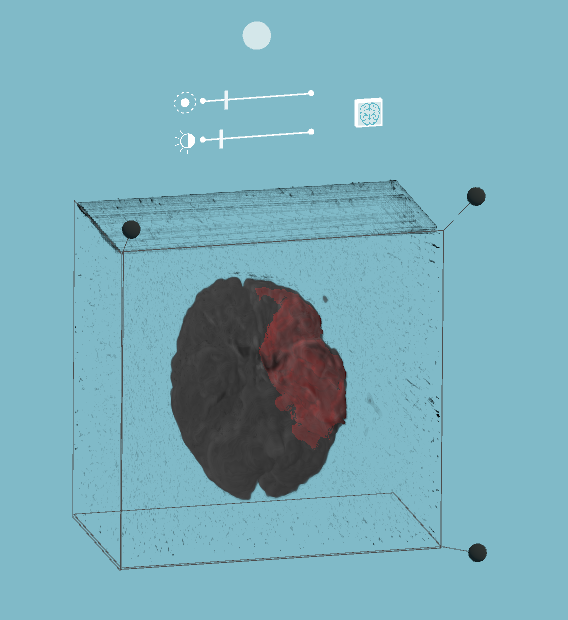
\includegraphics[width=0.5\linewidth]{images/mARt3d_2.png}
	\caption{Die 3D-Darstellung eines MRT-Datensatzes mit angezeigter Maske. Die oberen Schieberegler kontrollieren Intentsität und Gammakorrektur des Renderings. Auch hier wird der markierte Bereich durch ein Icon ein- und ausgeblendet. Jede Ebene kann durch einen Anfassungspunkt verschoben werden.}
	\label{img:mARt3d}
	\source{Eigene Darstellung}
\end{figure}
\FloatBarrier

Dieses Bedienkonzept lässt sich allerdings nicht einfach in den zweidimensionalen Raum übertragen. Da jeweils nur die ausgewählte Schicht zu sehen ist und nicht das gesamte Volumen, hat der Nutzer keine Vorstellung davon wo in dessen Innern er sich befindet. Um ihm diese zu liefern, wird die Gesamtanzahl an schichten angezeigt, sowie die wievielte gerade ausgewählt ist. 
Die Bewegung durch die Schichten erfolgt außerdem entlang der Z-Achse, die durch den zweidimensionalen Kontext allerdings wegfällt. D.h. der Wechsel zwischen den Schichten durch Anfassen und Ziehen eines Kontaktpunktes entlang dieser, wie eben beschrieben, würde nicht in das Konzept passen. 
Weiterhin sollte es dem Nutzer möglich sein die Ebene ununterbrochen zu verschieben. Bei einer Bewegung entlang der Z-Achse müsste er sehr weit vorne anfangen und ist in der Tiefe durch die Länge seines Armes beschränkt. Es wäre möglich das Interaktionselement als Schieberegler in die XY-Achse zu legen, die Bedienung ist dabei allerdings oft ungenau und könnte dazu führen, dass der Nutzer den Fokus auf den Regler legt, anstatt auf das Bild, das er auswählen will. Eine bessere Variante stellt ein Rad dar, durch dessen Rotation man zwischen den Bildern wechseln kann. Dies entspricht eher der Bedienung einer Bildschirmanwendung mittels eines Mausrads und ist dem Nutzer somit bereits bekannt. Außerdem lässt sich so eine kontinuierliche Bewegung in beide Richtungen ermöglichen. Der Nutzer muss zur Steuerung lediglich die Hand und nicht den Arm bewegen, was eine genauere Manipulation erlaubt. 
Das Rad ist dabei ähnlich einer Wählscheibe konzipiert, die der Nutzer mit einer Kreisbewegung rotiert. Verglichen mit einem Drehknopf, wie z.B. einem Lautstärkeregler, unterstützt der größere Radius mehr Kontrolle. Zudem lässt sich eine endlose Bewegung ohne Umgreifen realisieren und die Bewegung ist vom System leichter erkennbar. 
Um dem Nutzer den Eindruck von haptischen Feedback zu vermitteln und den Zustand des Elements zu verdeutlichen, wird die Berührung und Bewegung des Rades durch den Einsatz von Farbe untermalt.

%http://blog.leapmotion.com/designing-cat-explorer/

Wie in Abschnitt \ref{maske} beschrieben, wird der markierte, vom Schlaganfall betroffene Bereich innerhalb des Volumens dargestellt. Da die Maske entweder angezeigt wird oder nicht, kann der Nutzer die gewünschte Darstellung erreichen, indem er einen Schalter bedient, der zwischen den beiden Zuständen wechselt. Dies ist in \textbf{U11} gefordert.

Zur besseren Sichtbarkeit bestimmter Bereiche fordert Anforderung \textbf{U14}, dass die Helligkeit und der Kontrast der MRT-Bilder einstellbar sind. Dies ist über einen Schieberegler steuerbar, der sich oberhalb der Darstellung befindet. 
Die Manipulation von Helligkeit und Kontrast wird dabei als Gammakorrektur im Shader implementiert. Der von Nutzer bestimmte Gammawert wird dazu als Exponent zur Bildfarbe genommen. 
In der 3D-Darstellung wird außerdem ein weiterer Schieberegler angezeigt, über den der Nutzer bestimmen kann, wie intensiv Voxel dargestellt werden sollen. Diese Intensität beeinflusst die Opazität der Voxel. Ist ein hoher Wert eingestellt, werden die äußeren und damit dunkleren Voxel mit geringer Opazität dargestellt, sodass sie die weiter innen liegenden Voxel verdecken. Eine niedrige Intensität hat zur Folge, dass die äußeren Werte ausgeblendet werden, sodass die inneren Strukturen deutlicher zu erkennen sind. Auf diese Weise kann der Nutzer die Umgebung des Gehirns ausblenden und nur das Organ selbst darstellen.
Die Bedienoberfläche zur Manipulation der 2D-MRT-Daten ist in Abbildung \ref{img:mARt2d} zu sehen.

Obwohl nicht in den Anforderungen beschrieben, würde die Manipulation des gekennzeichneten Bereichs mit denselben Optionen dem Nutzer helfen die Darstellung seinen Ansprüchen anzupassen. Dies kann ebenfalls über Schieberegler gesteuert werden. Um die Anwendung überschaubar zu halten wurde allerdings davon abgesehen.


\begin{figure}[!htb]
	\centering
	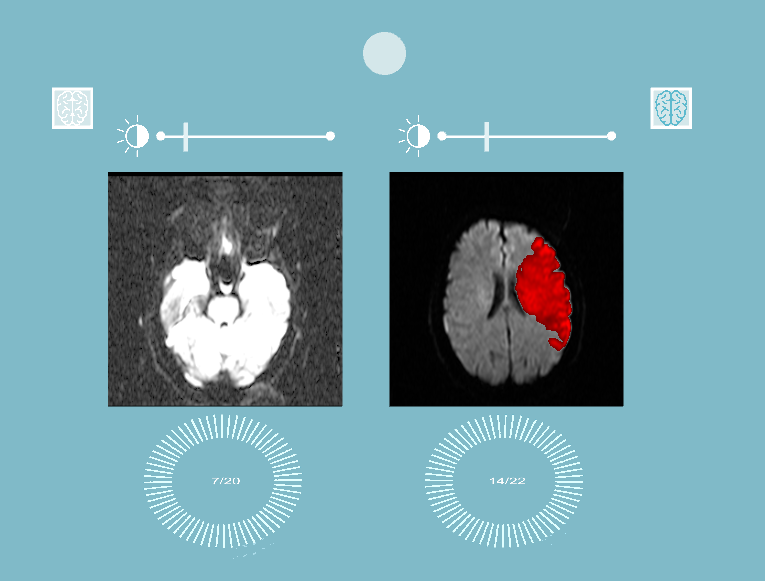
\includegraphics[width=0.7\linewidth]{images/mARt2d_2.png}
	\caption{Die zweidimensionale Darstellung von zwei MRT-Datensätzen, deren Manipulation nicht gleichgeschaltet ist. Über den oberen Schieberegler können Kontrast und Helligkeit per Gammakorrektur beeinflusst werden. Durch das Icon in der rechten Ecke kann der markierte Bereich ein- und ausgeblendet werden. Das Rad ermöglicht das Scrollen durch die Bildschichten. Die aktuelle Schicht wird in dessen Mitte angezeigt. }
	\label{img:mARt2d}
	\source{Eigene Darstellung}
\end{figure}
\FloatBarrier

% Zoom
Zu den geforderten Interaktionen gehört mit \textbf{U15} auch die Vergrößerung von Bildern, um dem Nutzer eine genaue Untersuchung zu erlauben. Bei der Vergrößerung handelt es sich im Grunde genommen um eine Skalierung des Bildes. Auch dies lässt sich gut mit einer direkten Handbewegung in Berührung mit der Darstellung umsetzten. Aus anderen Anwendungen sind Nutzern zwei Bedienmöglichkeiten dieser Funktionalität bekannt. Bei Bildschirmanwendungen wird oft das Mausrad zum Zoomen verwendet. Allerdings werden Räder bereits für andere Aktionen verwendet und ein mehrdeutiger Einsatz könnte zu Verwirrung führen. Von der Bedienung von Touchdisplays sind Nutzer weiterhin daran gewöhnt zu zoomen, indem sie den Bildschirm mit Daumen und Zeigefinger berühren und die Finger dann aufeinander zu oder voneinander weg bewegen. Diese Bewegung lässt sich gut in die Anwendung übertragen. Um ein eindeutigeres Ergebnis zu erhalten und dem Nutzer mehr Kontrolle zu geben werden statt zwei Fingern allerdings die beiden Hände verwendet. Wird das Bild von beiden Händen mit Daumen und Zeigefinder gegriffen kann es durch die Bewegung der Hände zueinander skaliert werden.

Um zu verhindern, dass zwei Darstellungen sich durch die Skalierung unterscheiden und die Anwendung überschaubar zu halten, ist eine Vergrößerung nur möglich, wenn ein einzelner Datensatz angezeigt wird. 
Das Vergrößern ist dabei als temporäre Manipulation konzipiert. Wenn der Nutzer einen zweiten Datensatz zur Visualisierung auswählt, wird der erste auf seine ursprüngliche Größe zurück gesetzt. Die Skalierung wird auch nicht in die andere Szene übertragen, wenn der Nutzer zwischen 2D und 3D wechselt. Dies kann dem Nutzer auch als bewusstes Zurücksetzten dienen, falls er die Skalierung beispielsweise versehentlich übertrieben hat.

% Verschieben
Die User Story \textbf{U16} fordert die Möglichkeit die Darstellung verschieben zu können. %Ersteres beschreibt dabei die Verschiebung im Raum, zweiteres eine Verschiebung der Darstellung. 
%Die beiden interaktionen wurden zu einer zusammen gefasst. 
Über den Bedienelementen einer Ansicht wird jeweils ein greifbares Objekt platziert. Durch das Greifen, Ziehen und Loslassen des Objektes kann der Nutzer die gesamte Darstellung verschieben. %Damit ist die Positionierung im Raum abgedeckt. 
Vergrößert der Nutzer eine Darstellung kann er dieselbe Verschiebung nutzen, um sich darin zu orientieren. 
%Zwar ist die Verschiebung auf die Armreichweite des Nutzers beschränkt, sofern er sich nicht im Raum bewegt, aber eine übermäßige Skalierung ist generell sowieso nicht erstrebenswert.
Um die Darstellung der Position des Nutzers weiterhin anpassen zu können, kann diese gedreht werden. Dazu dient ein weiteres Bedienelement, welches sich vor der Darstellung befindet. Um die Anwendung übersichtlich zu gestalten, erscheint dieses nur, wenn der Nutzer das erste Element ergriffen hat und somit seine Absicht demonstriert, die Darstellung zu bewegen. 
Sowohl Position als auch Rotation der Ansicht werden beim Szenariowechsel übernommen.
Die Bedienelemente zur Positionierung und Drehung der Ansicht sind in Abbildung \ref{img:3dPos} dargestellt. 

\begin{figure}[!htb]
	\centering
	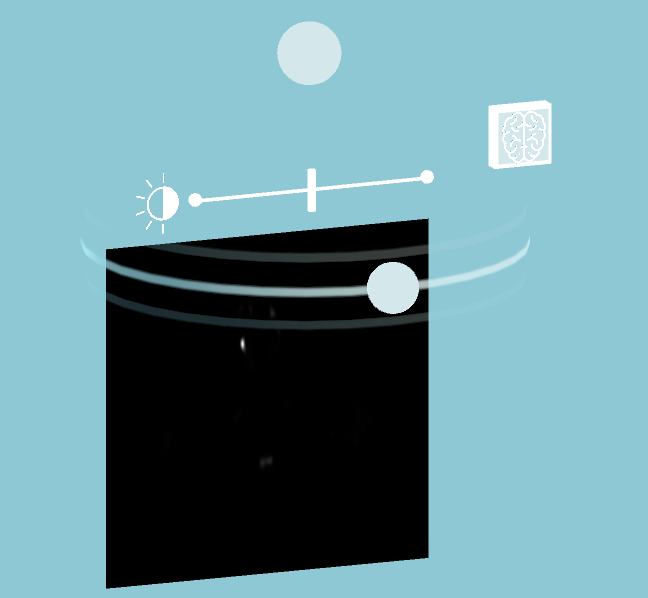
\includegraphics[width=0.5\linewidth]{images/mARt_turn.png}
	\caption{Die zweidimensionale Darstellung mit den beiden Bedienelementen zur Positionierung (oben) und Drehung (mitte).}
	\label{img:3dPos}
	\source{Eigene Darstellung}
\end{figure}
\FloatBarrier

Die Darstellung der MRT-Daten soll weiterhin nach \textbf{U17} die ihr gegebene Position behalten, sodass der Nutzer um sie herum gehen und von allen Seiten betrachten kann, oder an einem bestimmten Standpunkt verankern kann. Dies wäre vor allem in einem Multi-Nutzer-Szenario nützlich, in dem mehrere Nutzer gleichzeitig die Daten betrachten.
Die Bedienweise sollte sich durch diese Funktionalität nicht ändern. Zu deren Umsetzung gibt es verschiedene Ansätze, die in Abschnitt \ref{anchor} erläutert werden.

%Drehen
Entsprechend Anforderung \textbf{U13} soll die volumetrische Darstellung der MRT-Daten gedreht werden können. 
Die Drehung erfolgt dabei durch das Greifen des Volumens und Bewegen der Hand. Diese direkte Manipulation ist sehr intuitiv, wenn auch nicht unbedingt genau. Eine gradgenaue Drehung würde bei der Verwendung von mARt allerdings keinen erkennbaren Vorteil bringen. 
Wird das Volumen gedreht, drehen sich die Kontrollpunkte zum Verschieben der Bildebenen mit, um die lokale Verbindung zwischen diesen und der Ebene, die sie manipulieren zu erhalten. Würden sie sich nicht bewegen, wäre es schwer vorauszusehen, welcher Kontrollpunkt welche Ebene beeinflusst. 
Die UI wird von der Rotation allerdings nicht beeinflusst, da ihre Bedienung nur erschwert würde, wenn sie nicht annähernd orthogonal zur Blickrichtung des Nutzer verlaufen würde. 
Ebenso wie die Skalierung, ist die Rotation eine temporäre Manipulation, die beim Szenenwechsel zurückgesetzt wird.

Die User Story \textbf{U04} erfordert es weiterhin, dass Bilder im direkten Vergleich nebeneinander betrachtet werden können. Dies gilt sowohl für die zwei- als auch dreidimensionale Darstellung der Daten. Die User Stories \textbf{U05} und \textbf{U06} erfordern außerdem eine Möglichkeit für den Nutzer aus den vorhandenen Daten einzelne auszuwählen, die angezeigt werden sollen, sowie die Daten jeweils gleichzeitig oder einzeln zu manipulieren. 
Die Auswahl der Datensätze, sowie die Wahl ob diese synchron manipuliert werden sollen oder nicht, sind beide nicht Teil der direkten Manipulation des Bildes. Sie müssen deshalb nicht in dessen unmittelbarem Umfeld stehen und der Nutzer kann während dessen Bedienung auch auf diese den Fokus setzen.
 
Die Bedienung der entsprechenden Interaktionselemente sollte trotzdem intuitiv und schnell umzusetzen sein. Da die Option der Synchronizität abhängig ist von der Tatsache, ob ein oder mehrere Datensätze angezeigt werden, stehen die beiden Aktionen in Verbindung zu einander und werden deshalb in einem Menü vereint, das für beide Darstellungen verwendet wird. Dieses wird an der linken Hand des Nutzers verankert. Auf diese Weise kann es immer schnell erreicht werden und wird nicht unbeabsichtigt aus den Augen verloren. Gleichzeitig fördert es die Immersion der Anwendung, da der Nutzer quasi Teil von ihr wird. Ein Effekt, der in einer Bildschirmanwendung nicht umsetzbar wäre. 

Damit das Menü nicht während der Verarbeitung der Bilder stört, wird es nur dann eingeblendet, wenn der Nutzer seine Handfläche Richtung Kamera dreht und diese somit ansieht. Das \textit{Leap Motion} SDK bietet eine Beispielszene, die dies umsetzt.
Eine besondere Herausforderung bei der Konzeption des Menüs ist es, dieses möglichst einfach und platzsparend zu halten. Der Bereich der \textit{Leap Motion} Kamera, in dem die Hände erkannt werden ist beschränkt. Deshalb kann es bei einer Interaktionsfläche, die viel Raum davon einnimmt dazu kommen, dass der Nutzer versehentlich Knöpfe betätigt. 
Um den Umfang des Menüs in benutzbaren Dimensionen zu halten, wurde es auf drei Knöpfe reduziert. 
Die Liste der verfügbaren Datensätze kann darin allerdings nicht untergebracht werden. Deshalb kann sie bei Bedarf über einen der Knöpfe ausgeklappt werden. 
Indem der Nutzer einen Datensatz auswählt, wird dieser auf der Bildfläche angezeigt. Die Auswahl ist auf zwei Datensätze beschränkt. Zu viele gleichzeitig dargestellte Bilder würden unübersichtlich wirken und die Motivation hinter der User Story ist der direkte Vergleich zweier Bilder. Außerdem stellen mehr Bilder auch mehr Möglichkeiten dar diese in verschiedenen Kombinationen zu manipulieren. Dies hätte die Anwendung unnötig verkompliziert. 
Stattdessen wird die Synchronisierung der Manipulation über einen weiteren Knopf im Handmenü gesteuert. Dieser ist nur aktiv, wenn tatsächlich zwei Bilder angezeigt werden. Dann funktioniert er als Schalter. Indem der Nutzer ihn betätigt wird jeweils nur eine Benutzeroberfläche über beiden Bildern angezeigt oder sie wird dupliziert und für jede Darstellung eingeblendet. 
 
Schließlich kann der Nutzer durch das Handmenü auch zwischen der zwei- und dreidimensionalen Darstellung wechseln, wie es in \textbf{U09} beschrieben ist. Auf dem dafür zuständigen Button wird jeweils das Szenario angezeigt, in das gewechselt wird.
Laut \textbf{U10} sollen beim Wechsel die Manipulationen und Einstellungen möglichst erhalten bleiben. D.h. wenn in 2D zwei Datensätze angezeigt werden, einer mit und einer ohne Maske, sollte das nach dem Wechsel zu 3D ebenfalls so sein. 
Bis auf die genannten Ausnahmen werden die Einstellungen, die in einer Ansicht getätigt werden in die andere übernommen. Handelt es sich um Werte, die nur in einer der beiden Szenarios vorhanden sind, wie die Position der zusätzlichen Ebenen der 3D-Darstellung, werden diese ebenfalls gespeichert.
In Abbildung \ref{img:handUI} ist das ausgeklappte Menü, an der linken Hand dargestellt.

\begin{figure}[!htb]
	\centering
	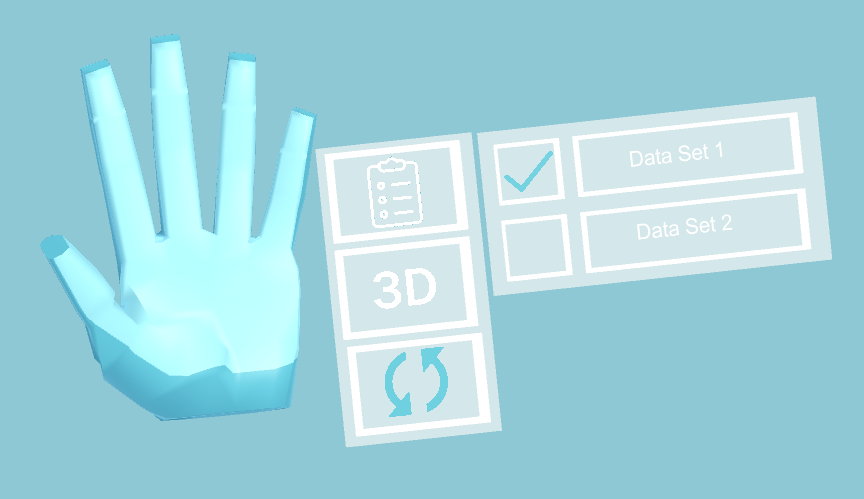
\includegraphics[width=0.7\linewidth]{images/handUI_2.png}
	\caption{Das ausklappbare Handmenü, das erscheint, wenn der Nutzer seine Handfläche zur Kamera dreht. Über die Knöpfe kann der Nutzer die angezeigten Datensätze auswählen (oben und Liste), zwischen 2D- und 3D-Darstellung wechseln (mitte) und die angezeigten Datensätze gleichschalten (unten). }
	\label{img:handUI}
	\source{Eigene Darstellung}
\end{figure}
\FloatBarrier

\subsection{Interaktion AR}

Die Interaktionen bleiben in der AR- und VR-Version der Anwendung gleich, da für beide die \textit{Leap Motion} zur Steuerung verwendet wird.
Im Gegensatz zum Einsatz in VR sind allerdings die realen Hände des Nutzers für diesen sichtbar, während er die Anwendung in AR bedient. Da durch die \textit{Leap Motion} die Hände zusätzlich virtuell simuliert werden, sieht der Nutzer vier Hände, was zuerst verwirrend wirken kann. 
Die Leap-Controller-Hände für den Nutzer unsichtbar zu machen, wäre zwar möglich, ist allerdings nicht die beste Vorgehensweise. Obwohl die \textit{Leap Motion} die Hände und Handbewegungen zuverlässig nachempfindet, verhalten die virtuellen Hände sich nicht ganz deckungsgleich zu den realen. Dies hängt auch damit zusammen, dass die \textit{Leap Motion} Kamera sich ein Stück vor oder über den Augen des Nutzers befindet, da sie am HMD befestigt ist. Dieses Problem wird auch in Abschnitt \ref{kombination} beschrieben.
Die Abweichungen der Simulation sind in einer VR-Anwendung deutlich weniger auffällig. Durch die Immersion der virtuellen Welt und dem Fehlen eines direkten Vergleichs mit der realen, entsteht beim Nutzer die Illusion, dass die virtuellen Hände sich genau dort befinden, wo er seine echten Hände vermutet. Dies ist durch die Dominanz der visuellen Wahrnehmung begründet, wie sie z.B. \cite{Azmandian16} beschreiben.

In AR entfällt diese Illusion. Da die beiden Handpaare aber nicht deckungsgleich sind, kann es dazu kommen, dass ein virtueller Finger einen Knopf trifft, während es ein realer nicht tut oder umgekehrt. Wenn der Nutzer die virtuelle Hand nicht sieht, würde dies den Eindruck von fehlerhaftem Verhalten hervorrufen. 
Aus diesem Grund werden die Leap-Controller-Hände auch in der AR-Anwendung angezeigt. Allerdings werden sie leicht transparent dargestellt, um dem Nutzer zu erlauben auch die dahinter liegende Umgebung wahrzunehmen. 
In Abbildung \ref{img:arHands} sind die Hände innerhalb der Anwendung abgebildet.

\begin{figure}[!htb]
	\centering
	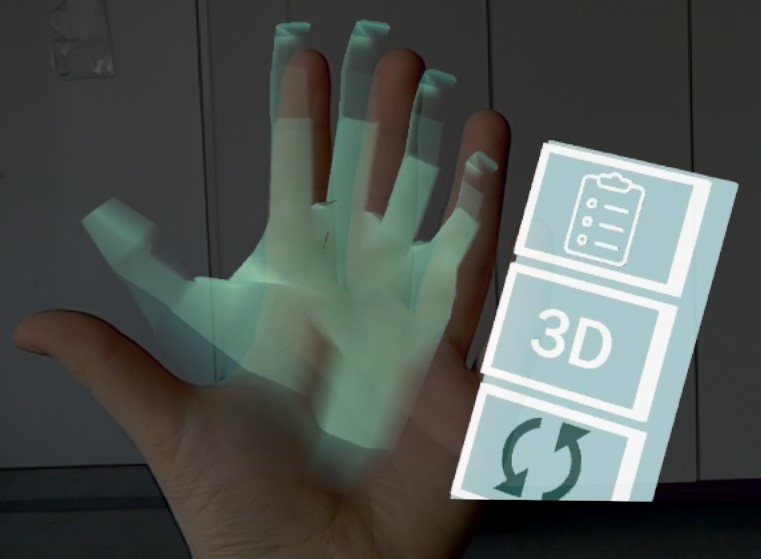
\includegraphics[width=0.5\linewidth]{images/AR_hand.jpg}
	\caption{Aufnahme aus der \textit{HoloLens}, die die augmentierte Hand des Nutzers zeigt.}
	\label{img:handUI}
	\source{Eigene Darstellung}
\end{figure}
\FloatBarrier


\section{Unterstützung von Dateiformaten} 

In den im Kapitel \ref{anforderung} beschriebenen Anforderungen ist durch \textbf{U19} und \textbf{U20} beschrieben, dass mARt gängige Dateiformate zur Speicherung von medizinischen Bilddaten, insbesondere NIfTI und DICOM unterstützt. Beide Formate wurden im Kapitel \ref{grundlagen} beschrieben. 
Um die MRT-Bilder verarbeiten und darstellen zu können, muss eine Parser oder Converter in das Programm eingebunden werden. 
Der Nutzer könnte dann über eine Schnittstelle die Daten direkt in die Anwendung laden, wo sie umgewandelt und angezeigt würden. 

In einer realen Arbeitsumgebung ist diese Funktionalität mehr als sinnvoll. Wie allerdings in Kapitel \ref{anforderung} beschrieben, soll es sich bei mARt in erster Linie um einen Prototyp handeln.
Der Fokus soll dabei auf der Darstellung der Daten und der Interaktion mit ihnen liegen. Da der zur Entwicklung und zum Testen zur Verfügung stehende Datensatz gering ist, ist die Nützlichkeit in diesem Szenario nicht gegeben. Der benötigte Zeitaufwand zur Implementierung wird somit nicht durch einen Mehrwert gerechtfertigt.
Weiterhin kann so die Komplexität und der Umfang der Anwendung gering gehalten werden, was es dem Nutzer erlaubt sich auf die Kernfunktionen zu konzentrieren. 

Durch den eingeschränkten verfügbaren Datensatz, konnte auch \textbf{U18}, nicht umgesetzt werden, da jeder Datensatz nur in einer Sequenz zur Verfügung steht.

Trotzdem können mehrere Datensätze in mARt dargestellt werden. Diese werden durch Verwendung von externer Bildsoftware manuell in PNG-Dateien umgewandelt und in die Anwendung integriert, bevor diese gebaut wird. 
Obwohl dieser manuelle Vorgang umständlich ist, ist er für den Zweck der Anwendung und den Umfang dieser Arbeit ausreichend.

% Implementierung

\chapter{Implementierung}
\label{implementierung}

Nachdem das Konzept der Anwendung beschrieben wurde, wird in den folgenden Abschnitten auf die Implementierung von mARt eingegangen. 

\section{Aufbau Struktur des Projektes}

Wie im Kapitel \ref{konzept} erläutert wurde, stellt mARt jeweils eine zwei- und dreidimensionale Darstellung der MRT-Daten zur Verfügung, zwischen denen gewechselt werden kann. Auf Grund der beschriebenen Hindernisse bezüglich der Leistungsfähigkeit der \textit{HoloLens} wurde die Anwendung sowohl für die \textit{HoloLens}, als auch als VR-Anwendung implementiert. Die AR-Anwendung kann dabei nicht für die \textit{HoloLens} bereitgestellt werden. Aus diesem Grund wird die nur auf dem Gerät abgespielt. In beiden Fällen handelt es sich im Kern um die selbe Anwendung, d.h. die Software sollte für beide Gräte entwickelt werden. 
Sowohl für die Entwicklung von VR- als auch AR-Anwendungen werden im Allgemeinen Spiele-Engines verwendet, da sie einen Editor bieten, um interaktive 3D-Anwendungen zu erzeugen, die in Echtzeit funktionieren. 
Zur Implementierung von mARt wurde \textit{Unity} von \cite{unity} verwendet. Die Engine gehört zu den meist genutzten auf dem Markt. Laut \cite{unityRelations} selbst, werden 60\% von AR/VR Inhalten mit \textit{Unity} entwickelt. Weiterhin ermöglicht \textit{Unity} die Entwicklung von Software für die meisten Plattformen. \textit{Unity} bietet viele nützliche Funktionen zur Entwicklung von interaktiven Anwendungen und wird außerdem von einer großen  Gemeinschaft genutzt, sodass neben einer detaillierten Dokumentation auch über Foren und Webartikel hilfreiche Informationen zur Entwicklung zur Verfügung stehen.

\textit{Microsoft} empfiehlt weiterhin \textit{Unity} zur Entwicklung für \textit{HoloLens}-Software zu nutzen \cite{unityHololens} und bietet mit \textit{Mixed Reality Toolkit} (MRTK) von \cite{holoToolkit} ein Framework, das \textit{HoloLens}-Funktionen innerhalb von \textit{Unity} zur Verfügung stellt.
\textit{Unity} verwendet C\# als Skriptsprache. Die Engine selbst ist allerdings in C++ geschrieben, wodurch effiziente Berechnungen zur Laufzeit ermöglicht werden.
\todo{Referenzen?}
%Wieso?

mARt wurde in \textit{Unity} entwickelt und sollte dann sowohl für die \textit{HoloLens} und als VR-Anwendung gebaut werden. Die Anwendung konnte allerdings nicht für die \textit{HoloLens} bereitgestellt werden. Diese Problematik wird in Abschnitt \ref{kombination} erläutert.
Um die \textit{Unity}-Anwendung auf dem VR-System abzuspielen, wird die \textit{SteamVR}-Software von \cite{steam} in das Projekt integriert. Um die Anwendung starten zu können muss sie auf dem jeweiligen Computer installiert sein.

\subsection{\textit{Unity} Projekt}

\textit{Unity} Projekte basieren auf 3D-Szenen. Innerhalb einer Szene können GameObjects platziert werden. Dabei kann es sich z.B. um 3D-Modelle handeln. Ein GameObject besitzt verschiedene Components, die dessen Eigenschaften und Verhalten bestimmen. Viele Funktionen und Eigenschaften werden von bereits in der Engine vorhandenen Components realisiert. Sogenannte Rigidbodys verleihen einem Objekt beispielsweise physikalische Eigenschaften, die von der Engine berechnet werden. Components können auch Skripte sein, die der Entwickler selbst verfasst hat. Über diese Skripte wird die Spiellogik und die Funktionalität der Anwendung definiert. 

Da mARt sich in die beiden Szenarien einer zwei- und dreidimensionalen Darstellung unterteilen lässt existiert für jedes Szenario eine Szene.
Viele der Funktionen sind allerdings ähnlich oder gleich, weshalb manche Skripte in beiden Szenen verwendet werden. 
Zusätzlich zu den beiden Szenen existiert eine Startszene Main/Preload.unity, in der ein GameObject namens appState liegt, über das bestimmt werden kann welche Szene zuerst geladen werden soll. In diesem Objekt werden auch die Zustände der Szenen gespeichert und so Manipulationen übertragen.
Die Szenen für die 2D-Darstellung sind 2DUI/main\_2D.unity und 2DUI/main\_2D\_AR.unity. Die für die 3D-Darstellung 3DUI/main\_3D.unity und 3DUI/main\_3D\_AR.unity.



\section{Shader in Unity}

Wie in Kapitel \ref{konzept} beschrieben wurde, wird das Volume Rendering der MRT-Daten in einem Shaders umgesetzt. An dieser Stelle soll ein Überblick über die Funktionsweise und den Aufbau von \textit{Unity}-Shadern gegeben werden. Aufbau und Funktionsweise sind in der \textit{Unity}-Dokumentation von \cite{unityDoku} beschrieben.

Wie ein Objekt in einer Szene gerendert wird hängt in \textit{Unity} davon ab, welches Material diesem zugewiesen ist. Das Material fungiert dabei als Behälter für sämtliche Parameter, die das Aussehen des Objektes beeinflussen, wie z.B. die Textur oder Farbe. Welche Parameter das Material besitzt und wie diese miteinander verrechnet werden bestimmt der Shader des Materials. Innerhalb des Shaders wird in Abhängigkeit zu den diesem übergebenen Werten die Farbe für jeden Pixel errechnet. 
% https://docs.unity3d.com/Manual/Shaders.html

Shader in \textit{Unity} sind in der \textit{Unity} eigenen Shader-Sprache Shader Lab geschrieben. Im Shader ist definiert welche Eigenschaften dieser besitzt und welche Sub- und Fallback-Shader er verwendet.
Die Eigenschaften sind die eben genannten Parameter, deren Werte dann über das Material gesetzt werden. Hier werden deren Namen, Typen, ihr Wertebereich sowie ihre Standardwerte definiert. 

Schließlich werden im Shader auch sogenannte Subshader definiert, die den eigentlichen Shader-Code enthalten.
Ein Shader kann mehrere Subshader enthalten für den Fall, dass einer der Shader von einem Gerät nicht unterstützt wird. Wird keiner unterstützt wird der Fallback-Shader verwendet. 
Neben dem Shader-Code besitzt ein Subshader Tags, die bestimmen wann und wie ein Shader von der Rendering-Engine gerendert werden soll. Dies kann sich beispielsweise auf die Reihenfolge beziehen, in der Objekte gerendert werden oder ob ein Objekt Schatten werfen soll. 
Nach den Tags folgt die Definition eines Pass. Als Render Pass wird der gesamte Prozess bezeichnet, der durchlaufen wird, um einen Pixel zu rendern. Angefangen bei der Berechnung einzelner Vertices eines Meshes über den Vertex-Shader bis zum Fragment-Shader. D.h. im Pass werden in verschiedenen Methoden die tatsächlichen Berechnungen beschrieben, die zum Aussehen jedes Pixels führen. 
Auch ein Pass kann zunächst wieder Tags enthalten, die bestimmen wann oder wie oft ein Pass durchlaufen werden soll. 
% Render setup ????
Dann folgt der Abschnitt, der den Shader-Code enthält. Dieser ist in Cg (C for Graphics)
\todo{REFERENZ} geschrieben, einer Shading-Sprache, die syntaktisch stark HLSL (High-Level Shading Language) ähnelt. 
Abhängig davon um welche Art von Shader es sich handelt, werden hier die notwendigen Funktionen implementiert. \textit{Unity} besitzt sogenannte Surface-Shader,  vereinfachte Shader, für die kein Beleuchtungsmodell implementiert werden muss. Andererseits können auch Unlit-Shader implementiert werden, in deren Pass Vertex- und Fragment-Shader definiert sind. 
Das Volume Rendering der MRT-Daten erfolgt durch einen Unlit-Shader. Auf die genaue Implementierung wird im Folgenden eingegangen. 

% https://docs.unity3d.com/Manual/SL-Shader.html
\todo{ P
REFERNZEN
}
\section{Grundlage der Implementierung}

Die in Kapitel \ref{anforderung} beschriebenen Anforderungen repräsentieren den Umfang der zu implementierenden Anwendung. 
Neben der Umsetzung der Anwendungslogik stellt vor allem die Implementierung der 3D-Darstellung durch Volume Raycasting einen hohen Aufwand dar. Um diesen in einem realisierbaren Rahmen zu halten, wurde ein bereits existierendes Programm als Basis für die zuletzt genannte Funktionalität verwendet.
Wie in Kapitel \ref{grundlagen} beschrieben wurde, gibt es bereits viele Implementierungen von Volume Raycasting zur Visualisierung von medizinischem Bildmaterial. 
Die dort genannten Unity-spezifischen Lösungen sind allerdings kostenpflichtig und/oder ihre Codebasis ist nicht einsehbar. Es wäre allerdings von Vorteil die Kontrolle über die Implementierung der 3D-Darstellung zu haben, um so die Möglichkeit zu haben, sie den Anforderungen entsprechend anpassen zu können.
Aus diesem Grund wurde die Open-Source-Implementierung von \cite{volumeRenderingGit} als Grundlage für die 3D-Darstellung verwendet, die unter der MIT-Lizenz steht.
Diese wurde erweitert, um die Anforderungen an mARt zu erfüllen. 
Im Rahmen der Arbeit wurden folgende Bestandteile implementiert:

\begin{itemize}
\item Erweiterung des Shaders (Maske, Beleuchtung)
\item Umwandlung von Bilddaten in 3D-Texturen und der Berechnung ihrer Gradienten
\item Anpassung der Bedienelemente an 3D-Szene
\item Anwendungslogik
\end{itemize}
Der fremde Code ist im Projekt gekennzeichnet.

\section{Volume Rendering}

Wie in Kapitel \ref{konzept} beschrieben wurde, wurde die 3D-Darstellung des Gehirns mit Hilfe von Volume Raycasting umgesetzt. 
Im Abschnitt \ref{rayCasting} wurde der theoretische Vorgang dieser Technik beschrieben. Dieser Abschnitt fokussiert sich auf die Implementierung der einzelnen Schritte.

Die volumetrische Darstellung des Gehirns wird mit drei Skripten erzeugt. Zuerst wird in VolumeRendering/Scripts/VolumeRendering.cs das Mesh des Würfeln generiert. Hier werden auch die Parameter aktualisiert, die für das Rendering relevant sind, wie z.B. die 3D-Textur oder Farbe, sowie die Parameter, die durch die Nutzerschnittstelle manipuliert werden können. 
Die Parameter werden an den Shader VolumeRendering/Shader/VolumeRendering\_Diffuse\_Mask.shader übergeben, in dem das Rendering definiert ist. Der Cg-Code, der den Vertex- und Fragment-Shader implementiert ist dabei in ein eigenes Skript VolumeRendering/Shader/VolumeRendering\_Diffuse\_Mask.cginc ausgelagert.

\subsection{Volume Raycasting}
\label{3dImplementierung}
Im Fragment-Shader des VolumeRendering/Shader/Volume\_Diffuse\_Mask.sh Shaders wird zunächst ein Strahl definiert, der von dem aktuell betrachteten Vertex aus von der Kameraposition in die Welt geschossen wird. In einem selbst definierten struct werden die maximalen und minimalen Werte definiert, aus denen sich die Eckpunkte des dargestellten Quaders zusammensetzten. Anschließend wird geprüft, ob der Strahl den Würfel schneidet. 

%-----------Intersect-----------
%Dies geschieht indem zuerst die Inverse der Strahlrichtung ermittelt wird. Die Inverse eines Vektors $v$ ist $v^-1$ und da $v^-x=\frac1}{v^x}$, ergibt sich die Inverse des Richtungsvektors des Strahls indem $1$ durch die dividiert wird.
% AABB, axis aligend etc? intersection formula REFERENZ
Um die Schnittpunkte des Strahls zu ermitteln nimmt man an, dass die sechs Seiten des Würfels auf jeweils sechs Ebenen liegen, wobei davon zwei immer parallel sind. Zuerst werden alle Schnittpunkte des Strahls mit diesen Ebenen berechnet und dann geprüft, ob die Schnittpunkte innerhalb des Würfels liegen.
Der Würfel wird durch zwei Eckpunkte beschrieben. Da der Würfel Koordinaten von -0,5 bis 0,5 hat können wir hierfür die jeweils kleinsten und größten Koordinaten nutzen. 
Die Schnittpunkte des Strahls, mit den X-, Y- und Z-Ebenen ergeben sich durch das Umstellen der Formel, die einen Strahl beschreibt:

\begin{align}
p=r_{Ursprung}+t*r_{Richtung}
\end{align}

$r_{Ursprung}$ ist dabei der Ursprung des Strahls und $r_{Richtung}$ seine Richtung. $p$ ist ein Punkt auf dem Strahl und $t$ ein Parameter, der bestimmt wie weit der Punkt vom Ursprung entfernt ist.

Um die Schnittpunkte mit den Ebenen zu erhalten wird die Formel nach $t$ umgestellt:

\begin{align}
t=(p-r_{Ursprung})/r_{Richtung}
\end{align}

Für $p$ werden jeweils die beiden Eckpunkte des Würfels, die jeweils auf drei der Würfelebenen liegen, eingesetzt.
Dadurch sind insgesamt sechs $t$s und damit sechs Schnittpunkte mit den Ebenen bekannt. Zwei für jedes Ebenenpaar. Die Entfernungen werden in den zwei dreidimensionalen Vektoren $t_{unten}$ und $t_{oben}$ gespeichert. Durch den Vergleich der t-Vektoren wird festgelegt, welcher Eckpunkt und damit welche zweier paralleler Ebenen weiter vorne liegt. 
% Was wenn Strahl parallel zur Ebene ist??
Jetzt muss bestimmt werden, ob diese Schnittpunkte sich innerhalb des Würfels befinden.
Dazu werden jeweils die x-, y- und z-Werte der t-Vektoren untereinander verglichen. Für das $t$ der näher gelegenen Ebene wird der maximale, für den weiter entfernten der minimale Wert bestimmt. Ist der Wert des näheren $t$s größer als der des entfernten, schneidet der Strahl den Würfel nicht. Andersherum tut er es.
Das Verhältnis der Schnittpunkte zueinander und wie dieses durch den Verlauf des Strahls bestimmt wird ist in Abbildung \ref{img:rayBoxHit} dargestellt.

\begin{figure}[!htb]
	\centering
	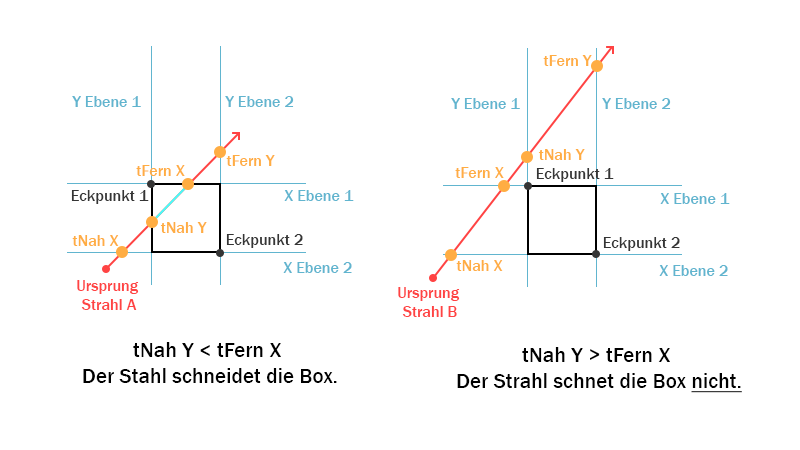
\includegraphics[width=0.9\linewidth]{images/rayBox.png}
	\caption{Zweidimensionale Darstellung, wie ein Strahl durch einen Würfel (links) und daran vorbei (rechts) verläuft. Die Schnittpunkte des Strahls (gelb) mit den Würfelebenen (blau) sind eingezeichnet. Der Vergleich derer Abstände zum Ursprung des Strahls (rot) zeigt, ob der Strahl den Würfel schneidet oder nicht.}
	\label{img:rayBoxHit}
	\source{Eigene Darstellung}
\end{figure}
\FloatBarrier

%----------------------------------------
Die beiden t-Werte werden als $t_{nah}$ und $t_{fern}$ gespeichert.
Mit dem Ursprung des Strahls und $t_{fern}$ werden Anfang, Ende und die Länge des Strahls berechnet. Mit Hilfe der Länge kann ermittelt werden um wie weit pro Iteration am Strahl entlang gegangen werden soll. Dadurch wird der Strahl nur bis zu seinem Austritt aus dem Würfel abgetastet. 

In einer for-Schleife wird jeder Strahl nun abgetastet. In jeder Iteration wird jeweils ein Punkt betrachtet. Der Punkt verschiebt sich entlang des Strahls um die zuvor berechnete Distanz.
Für jeden Punkt werden zuerst die Texturkoordinaten berechnet.
Für die Koordinaten werden dann die jeweiliges Isowerte aus der 3D-Textur gelesen, die zuvor mit den MRT-Bildern befüllt wurde.

%---------------SAMPLE VOLUME-------------
Hierbei werden lediglich die Texturkoordinaten als Indices für die Textur verwendet. 
Der Isowert ist dabei im Alphakanal der Textur gespeichert. Da es sich nicht um eine Farbe sondern nur einen Grauwert handelt, können die anderen Farbkanäle der Textur mit dem Gradienten des jeweiligen Pixels befüllt werden. Darauf wird im Abschnitt \ref{gradienten} genauer eingegangen.

Der Isowert wird außerdem noch mit der Intensität multipliziert, die der Nutzer beeinflussen kann.
An dieser Stelle wird aber auch geprüft, ob der betreffende Punkt überhaupt zu sehen ist oder aufgrund der verschiebbaren Schichten nicht sichtbar sein sollte. 
Dazu wird zuerst der aktuell betrachtete Punkt mit der Rotationsmatrix des Volumens multipliziert.
Der Punkt wird dann mit den von Nutzer eingestellten minimalen und maximalen X-, Y-, und Z-Werten der verschiebbaren Schicht verglichen, die den sichtbaren Bereich definieren. Das Ergebnis des Vergleichs wird dabei in einer Variable gespeichert. Ist der Punkt kleiner als das Minimum oder größer als das Maximum wird 0 gespeichert, ansonsten 1. 
Die beiden Werte werden anschließend mit dem Isowert multipliziert. Ist einer der Werte 0, ist auch der ermittelte Isowert 0, was im Alphakanal totale Transparenz bedeutet. 
Das Ergebnis dieser Berechnung wird zunächst jedem Farbkanal zugewiesen.
%-----------------------------------------

An dieser Stelle wird über die Transferfunktion der entsprechende Alphawert aus der zugehörigen Textur gelesen. Dazu wird der Isowert als Index verwendet. Die Funktionsweise und Implementierung der Transferfunktion wird in der Sektion \ref{transfer} beschrieben.
% Bezug Transferfunktion!
Die Transferfunktion wird nur abgerufen, wenn der Isowert nicht 0 ist, da sonst die Transparenz überschrieben würde.
% Tranferfunktion bei index 0 auf 0000 setzen??
Ist die Farbe bekannt, wir der betrachtete Voxel illuminiert. Dies ist in der Sektion \ref{illumination} beschrieben. 
Der Alphawert der so erhaltenen Farbe wird noch einmal halbiert, um die Darstellung semi-transparent erscheinen zu lassen.
% WARUM
Schließlich wird der erhaltene Farbwert mit den vorhergehenden verrechnet. Die Komposition erfolgt dabei von vorne nach hinten, da der Strahl in dieser Richtung abgetastet wird, nach der in Kapitel \ref{grundlagen} beschriebenen Formel.
% Referenz GPU Gems
Wenn diese Farbe einen zuvor definierten Schwellenwert überschreitet wird die Schleife abgebrochen. 
Die Farbe wird schließlich noch auf einen Wert zwischen 0 und 1 festgesetzt und mit der Farbe der Maske verrechnet, die auf dem selben Weg aber ohne die Verwendung einer Transfertextur bestimmt wurde.

\subsection{Transferfunktion}
\label{transfer}

Wie beschrieben, wird die Transfertextur im Shader ausgelesen. Vorher wird sie von dem Skript 3DUI/Scripts/CreateTransferColorTexture.cs erzeugt, welches beim Ausführen der Szene 3DUI/Scenes/Load3DTexture.unity ausgeführt wird.
Um eine Transfertextur zu erzeugen, werden zunächst zwei Key-Value-Listen definiert, in denen über Kontrollpunkte bestimmte Isowerte einem Farb- oder Opazitätwert zugewiesen werden. Mit Hilfe einer Schleife wird dann eine 2D-Textur mit den Dimensionen 256 und 1 erstellt. Dabei wird für jeden X-Wert der Textur geprüft, ob er größer oder gleich dem Isowert des betrachteten Kontrollpunktes ist. Ist dies der Fall, wird der Pixel der Textur mit dem entsprechenden Wert besetzt. Dies geschieht für alle Kontrollpunkte.
Die Textur wird dann als 2D-Textur abgespeichert. Da allein die Isowerte als Index für die Zuordnung verwendet werden, handelt es sich eigentlich um eine eindimensionale Transferfunktion. 
Allerdings werden von \textit{Unity} keine 1D-Texturen als Shader-Eigenschaften unterstützt. Da die Verwendung einer 2D-Textur aber keine Nachteile aufweist, wird stattdessen eine 2D-Textur verwendet, die eine einzige Y-Koordinate besitzt. 
Die Textur wird dann über das Material an den Shader übergeben. Wie im Abschnitt \ref{3dImplementierung} beschrieben, wird die Textur dann mit Hilfe eines Index ausgelesen.

Die Erstellung einer passenden Transfertextur ist allerdings, wie beschrieben, sehr schwierig und es konnte im Rahmen dieser Arbeit keine sinnvollen Kontrollpunkte zur Einfärbung des Volumens ermittelt werden. Aus diesem Grund wird nur der Alphawert der Transferfunktion verwendet. Auf diese Weise werden irrelevante Bildinformationen, wie Umgebungsrauschen und der Schädel ausgeblendet, wobei die Struktur des Hirninneren bestehen bleibt. 

\subsection{Beleuchtung}
\label{illumination}

Das Volumen wird mit mit dem Phong-Beleuchtungsmodell illuminiert, wodurch es mehr Plastizität erhält. Das Modell wurde bereits in Kapitel \ref{grundlagen} detailliert beschrieben. Deshalb wird an dieser Stelle nur auf die Umsetzung im Shader eingegangen.
% Referenz? warum nicht blinn?
Wie beschrieben setzt sich das Modell aus drei Komponenten zusammen: Der ambienten und der diffusen Beleuchtung, sowie der spiegelnden Reflexion. Die Komponenten werden zusammen addiert, wodurch die endgültige Farbe entsteht. 
Die Koeffizienten werden im Shader durch Farben repräsentiert. Der diffuse Koeffizient ist dabei der vorher aus der Transferfunktion gelesene Farbwert. Um diesen nicht durch die ambiente Beleuchtung zu verfälschen, wird er mit einem konstanten Faktor multipliziert, um eine abgedunkelte Farbe zu erhalten, die als ambienter Wert verwendet wird. Die Reflextion wird weiß dargestellt.
%Als Reflexionsexponent hat sich der Wert ?10? als am besten erwiesen.
Um die Reflexion berechnen zu können müssen außerdem der Lichtvektor und die Normale bekannt sein.
Wie bereits erläutert, wird der Gradient eines Voxels als Normale verwendet. 
Der Vektor zum Licht wird aus der in \textit{Unity} eingebauten Shader-Variable \_WorldSpaceLightPos0 ausgelesen.
\todo{P Unterscheidung direktionales und Punktlicht?}

\subsection{Gradientenberechnung}
\label{gradienten}


Die Gradienten werden vor dem Start der Anwendung berechnet und zusammen mit den Isowerten in eine 3D-Textur geschrieben. Der Gradientenvektor wird dabei in den RGB-Kanälen gespeichert und der Isowert im Alpha-Kanal, da es sich nur um einen einzelnen Wert handelt. 

Die Berechnung der Gradienten erfolgt im selben Schritt, wie das Übertragen der Skalarwerte aus den Bilddaten in eine 3D-Textur.
Dafür werden alle Bilddateien in einem Dateiverzeichnis, auf das ein vorher definierter Pfad zeigt, ausgelesen und in ein Array übertragen, das der Größe der Bilder entspricht. Die dritte Dimension des Arrays wird durch die Anzahl der Bilder bestimmt. 

Entsprechend der in Kapitel \ref{grundlagen} beschriebenen Finite-Differenzen-Methode, werden durch eine Convolution die Gradienten für jeden Farbwert berechnet und ebenfalls in ein Array gespeichert.
Das Gradientenarray wird anschließend mit Hilfe eines Gauß-Filters mit einer Kernelgröße von 5 und $\sigma=5.5$ geglättet, bevor die Werte in eine 3D-Textur gespeichert werden. 

Diese wird im Asset-Verzeichnis 3DTextures des Projektes abgelegt. Sie werden in der Szene referenziert, um bei Bedarf an einen Shader übergeben zu werden, der den entsprechenden Datensatz darstellt. 

\section{\textit{HoloLens}-spezifische Implementierung}
\label{plattformen}

\subsection{\textit{HoloLens}-Demo}
Im Rahmen der Arbeit wurde neben der endgültigen Anwendung zuerst auch eine prototypische Demo-Anwendung entwickelt, die die \textit{HoloLens}-eigenen Gesten genutzt hat. Die Anwendung hat eine zweidimensionale Darstellung der MRT-Bilder als Hologramm in den Raum projiziert, welches der Nutzer durch \textit{HoloLens}-eigene Gesten manipulieren konnte. Dabei wurden alle vorhandenen Manipulierungsformen eines Hologramms abgedeckt, sowie das Scrollen durch die Bildschichten. Um die \textit{HoloLens}-Gesten zu Nutzen wurde das \textit{HoloToolkit} verwendet. 
Anhand dieser Demo sollte geprüft werden, ob die Interaktionsmöglichkeiten, die die \textit{HoloLens} bietet ausreichend sind, um einem Neurologen die effektive Untersuchung von MRT-Bildern zu ermöglichen.
Weiterhin konnten durch das Testen einer realen Anwendung die Erwartungen und Anforderungen eines Arztes an mARt noch weiter spezifiziert werden.  

Wie im Kapitel \ref{konzept} erläutert, haben sich die Gesten der \textit{HoloLens} zwar als ausreichend erwiesen, machten aber die Verwendung von weiteren Bedienelementen notwendig. Der Wechsel zwischen den Manipulationsarten wurde über ein ausklappbares Menü realisiert. Alle Manipulationen erfolgen über \textit{Air tap} und das Bewegen der Hand. Bei eingeklapptem Menü kann der Nutzer so durch die Darstellung scrollen. Aus den beschriebenen Gründen wurde für die endgültige Implementierung der Anwendung die \textit{Leap Motion} in das System integriert.
% Genauer auf Implementierung eingehen
Der Prototyp wurde in der Szene 2DUI\_HololensDemo/Scenes/HololensDemo.unity realisiert und eine Datei zur Bereitstellung für die \textit{HoloLens} sowie ein Video der Anwendung ist im Ergänzungsmaterial zu finden.
Die Demo ist in Abbildung \ref{img:prototyp} dargestellt.

\begin{figure}[!htb]
	\centering
	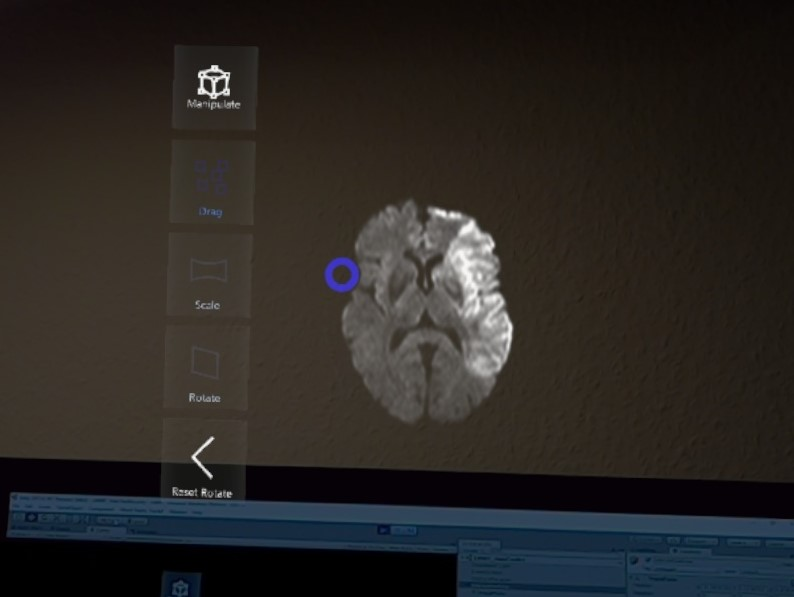
\includegraphics[width=0.5\linewidth]{images/hololens_prototyp.jpg}
	\caption{Aufnahme aus der \textit{HoloLens} von der \textit{HoloLens}-Demo, die Interaktionen ausschließlich über \textit{HoloLens}-Gesten realisiert.}
	\label{img:prototyp}
	\source{Eigene Darstellung}
\end{figure}
\FloatBarrier

\subsection{Positionierung im Raum}
\label{anchor}

Im Kapitel \ref{konzept} wurde bereits erwähnt, dass die dauerhafte Positionierung im Raum, wie sie \textbf{U17} fordert, auf unterschiedliche Weise implementiert werden kann. 
Die \textit{HoloLens} bietet diese Funktionalität in Form von Spatial oder World Anchors. Das Gerät besitzt einen internen Speicher für Anker, die von einer Anwendung angelegt werden, den sogenannten Anchor Store. Durch interne Prozesse bestimmt die \textit{HoloLens} in welchem Raum sie sich gerade befindet. Wird ein World Anchor in diesem Raum abgelegt, wird dessen Standort im Anchor Store gespeichert und behält somit immer seine Position im Raum, auch wenn der Nutzer sich bewegt und über mehrere Sitzungen hinweg. Nachdem ein World Anchor beim Start der Anwendung geladen wird, kann er an ein Objekt, wie ein 3D-Modell anhängt werden, sodass das Objekt an der Position des Ankers dargestellt wird. 

Ohne die Verwendung eines World Anchors wird die 3D-Szene und alle Objekte darin an der \textit{HoloLens} ausgerichtet, die den Nullpunkt der Szene darstellt. Durch die unterschiedliche Ausrichtung kommt es bei der Positionierung der Darstellung in der AR-Anwendung zu Komplikationen, sobald zwischen 2D- und 3D-Szene gewechselt wird. 

Der Anchor Store ist allerdings nur auf der \textit{HoloLens} verfügbar. Wie bereits erläutert wurde, wird die Anwendung im Rahmen dieser Arbeit aber nur auf der \textit{HoloLens} abgespielt, aber nicht für sie bereitgestellt. Dementsprechend ist ein Zugriff auf den Anchor Store nicht möglich. Dasselbe gilt für eine Verwendung der Anwendung in einem VR-System.

Als Alternative dazu können die Daten mit Hilfe eines Markers in den Raum projiziert werden, wie es im Kapitel \ref{grundlagen} beschreiben wurde. \textit{Unity} bietet hierfür das \textit{Vuforia}-Plugin, welches genau das umsetzt. Hierzu können Marker definiert werden, die das Programm erkennt und die diesen zugeordneten GameObjects anzeigt. 
\textit{Vuforia} ist für AR-Anwendungen gedacht und funktioniert durch eine Kamera, die den Marker erkennt. Deshalb kann die Funktion von einer \textit{Vive} nicht genutzt werden, von einer \textit{Vive Pro} jedoch schon, da diese über einen Mixed Reality Modus verfügt. Auch \textit{HoloLens}-Anwendungen können \textit{Vuforia} nutzen. 
Im zeitlichen Rahmen der Arbeit konnte dieses Funktionalität allerdings nicht mehr umgesetzt werden.

\section{Implementierung der Nutzereingabe}

\subsection{Verwendung der \textit{Leap Motion}}

Damit die \textit{Leap Motion} Kamera in einer Anwendung verwendet werden kann, muss das von \cite{orion} zur Verfügung gestellte SDK \textit{Orion} eingebunden werden. Das \textit{Core SDK} ist dabei zur Erkennung und Verwendung des Gerätes notwendig, während ein erweiterndes Paket Funktionen und Beispiele bietet, wie verschiedene Bedienelemente in eine Anwendung integriert werden können, die auf die Controller, also die Hände des Nutzers reagieren.
Meistens funktioniert dies indem einzelne Skripte, die das gewünschte Verhalten implementieren, als Components an GameObjects angehangen werden. Die Skripte lösen dann bestimmte Events oder Methoden aus, die mit den Funktionalitäten der Anwendung verknüpft werden. 

\subsection{Kombination von \textit{Leap Motion} mit \textit{Vive}/\textit{HoloLens}}
\label{kombination}

Sowohl \textit{Vive} als auch \textit{HoloLens} sollen in Verbindung mit der \textit{Leap Motion} funktionieren. Dazu muss zum Einen die \textit{Leap Motion} Kamera in beide Systeme integriert werden und zum Anderen die Funktionalität in die jeweiligen \textit{Unity} Szenen eingebaut werden. 

Das Einbinden der \textit{Leap Motion} in eine VR Anwendung, sowie die Kombination mit dem \textit{Vive} Headset sind unproblematisch. Das \textit{Orion} SDK der \textit{Leap Motion} unterstützt den Einsatz in VR-Szenen. Sofern \textit{SteamVR} installiert und eine VR-Brille angeschlossen ist, ist kein größerer Aufwand nötig, um die Hände des Nutzers in VR anzuzeigen. 
Die Integration in das VR-System ist vergleichbar einfach. Die \textit{Leap Motion} Kamera wird vorne auf dem HMD über der eingebauten Kamera befestigt und ihre Kabel zusammen mit den anderen der Brille über den Kopf des Nutzers geführt. 

Dagegen bringt die Verbindung von \textit{Leap Motion} und \textit{HoloLens} einige Herausforderungen mit sich. Zunächst ist in einer \textit{HoloLens}-Szene nur eine Kamera, die des HMDs, vorgesehen. Das Vorhandensein einer zweiten Kamera, wie die der \textit{Leap Motion} würde beim Erstellungsprozess zu Fehlern führen, sodass das Bereitstellen des Programmes für die \textit{HoloLens} nicht möglich ist.
Die \textit{Leap Motion} wird über ihr Kabel mit Strom versorgt. Sie kann also im Gegensatz zu der \textit{HoloLens} nicht kabellos funktionieren. 
Über das Kabel werden außerdem die von der \textit{Leap Motion} Kamera erfassten Daten weitergeleitet, die dann verarbeitet werden. Die dafür notwendige Software ist nicht für die \textit{HoloLens} verfügbar und es ist fragwürdig, ob sie die dafür notwendige Rechenleistung besitzt. 

Aus diesen Gründen muss die \textit{Leap Motion} während des Betriebs per Kabel mit einem Rechner verbunden sein. Um das Gerät trotzdem in Verbindung mit der \textit{HoloLens} nutzen zu können, müssen entweder die Sensordaten der \textit{Leap Motion} an die Anwendung in der \textit{HoloLens} übertragen werden oder die gesamte Anwendung läuft auf dem Rechner und wird zur Wiedergabe an die \textit{HoloLens} übermittelt. Beides geschieht über Wlan.

Die Übertragung der Sensordaten ist dabei um einiges aufwändiger und erfordert die Integration weiterer Tools. Es existieren einige Lösungsansätze für dieses Problem, beispielsweise von \cite{hololensGithub}. Auf Grund des beschränkten Zeitraums dieser Arbeit wurde dieser Ansatz allerdings nicht implementiert.
Stattdessen wird die Anwendung lediglich auf der \textit{HoloLens} wiedergegeben. Dazu wird die \textit{Hololens}-App \textit{Holographic Remoting Player} von \cite{remoteApp} genutzt. Die Anwendung wird dabei direkt aus dem \textit{Unity}-Editor übertragen.
Die Wiedergabequalität der Anwendung ist dabei abhängig von der Stabilität der Wlan-Verbindung.

Auch das Anbringen der \textit{Leap Motion} an das HMD ist bei der \textit{HoloLens} umständlicher als bei der \textit{Vive}. 
Da die \textit{Vive} einen undurchsichtigen Bildschirm besitzt, kann die \textit{Leap Motion} Kamera einfach vorne auf der Brille befestigt werden. Die Form des Gerätes bietet dazu ausreichend Fläche.
Bei der \textit{HoloLens} sollte der Bildschirm, durch den der Nutzer sieht nicht verdeckt werden. Eine Installation im oberen Teil der Frontseite ist ebenfalls nicht umsetzbar, da dieser von den \textit{HoloLens}-Kameras eingenommen wird, die die Umgebung und Nutzergesten verfolgen.
Somit ist die einzige sinnvolle Möglichkeit, die \textit{Leap Motion} auf der \textit{HoloLens} zu platzieren. Hierbei muss sie außerdem nach vorne geneigt werden, um die Hände des Nutzers in der Anwendung möglichst genau an den realen Händen auszurichten. 

% Ergebnisse


%\chapter{Ergebnisse}
\section{Ergebnisse}
\label{ergebnisse}

Die VR-Anwendung ist als ausführbare Datei im Ergänzungsmaterial zu finden. Da die \textit{HoloLens}-Anwendung, wie in Kapitel \ref{konzept} erläutert, nicht für diese bereitgestellt werden konnte, existiert hierfür keine ausführbare Datei. Allerdings wurde in der ReadMe.txt Datei des Projektes, welches sich ebenfalls im Ergänzungsmaterial befindet beschrieben, wie die Anwendung auf der \textit{HoloLens} abgespielt werden kann. 
Weiterhin ist dort ein Video enthalten, das die Funktionen und Bedienung der Anwendung zeigt.
Die Interaktionslemente wurden wie in Kapitel \ref{konzept} beschrieben implementiert. Neben ihrer Beschreibung sind dort auch Abbildungen der Benutzerelemente zu finden. 


\subsection{3D-Darstellung}

In Abschnitt \ref{3dImplementierung} wurde erläutert, wie die 3D-Darstellung mit Hilfe von Volume Raycasting erzeugt wurde. 
Dazu wurde der Alphawert einer Transfertextur genutzt, um das Rauschen in der Umgebung des Gehirns zu entfernen und die Gehirnform eindeutiger herauszustellen. Dies führt allerdings auch zu Artefakten, dem sogenannten Holzmaserungseffekt. Da allerdings die Darstellung der inneren Strukturen des Gehirns im Vordergrund steht, wurde sich für eine Darstellung entschieden, die durch Reduzierung der Umgebung den Fokus auf das Gehirn erlaubt. 
Im Abbildung \ref{img:resultsDWI} sind die beiden Datensätze mit und ohne die Verwendung einer Transferfunktion abgebildet. Durch Manipulation der Intensität kann bestimmt werden, in welcher Opazität das Gewebe gerendert werden soll, was vor allem das äußere Gewebe beeinflusst. Die Intensität der Renderings in der Abbildung ist in allen Fällen gleich.
Es ist anzumerken, dass die Qualität der Daten sich unweigerlich auf die Qualität des Renderings auswirkt. Die vorgegebenen Datensätze des Gehirns weisen ein hohes Maß an Bildrauschen auf. Außerdem wurden die Schichten offenbar in Abständen solcher Größe gescannt, dass die Interpolation zwischen den Schichten Aktefakte ausweist. Auch dies in in Abbildung \ref{img:resultsDWI} zu sehen.

\begin{figure}[!htb]
	\centering
	\includegraphics[width=0.9\linewidth]{images/dwi_results.png}
	\caption{Rendering der zur Verfügung gestellten Datensätze durch den in mARt verwendeten Shader mit gleicher Intensität. a) Datensatz 1 ohne Transferfunktion b) Datensatz 1 mit Transferfunktion c) Datensatz 2 ohne Transferfunktion d) Datensatz 2 mit Transferfunktion}
	\label{img:resultsDWI}
	\source{Eigene Darstellung}
\end{figure}
\FloatBarrier
  
Aus diesem Grund wurden testweise auch andere Daten mit dem selben Shader gerendert. Das Ergebnis ist dabei von besserer Qualität als mit den Gehirndaten. Die Verwendung der Transferfunktion ist nicht notwendig, um die Darstellung deutlicher zu machen. In Abbildung \ref{img:resultsVisMale} ist der Datensatz eines Kopfes mit und ohne Transferfunktion dargestellt.
  
\begin{figure}[!htb]
	\centering
	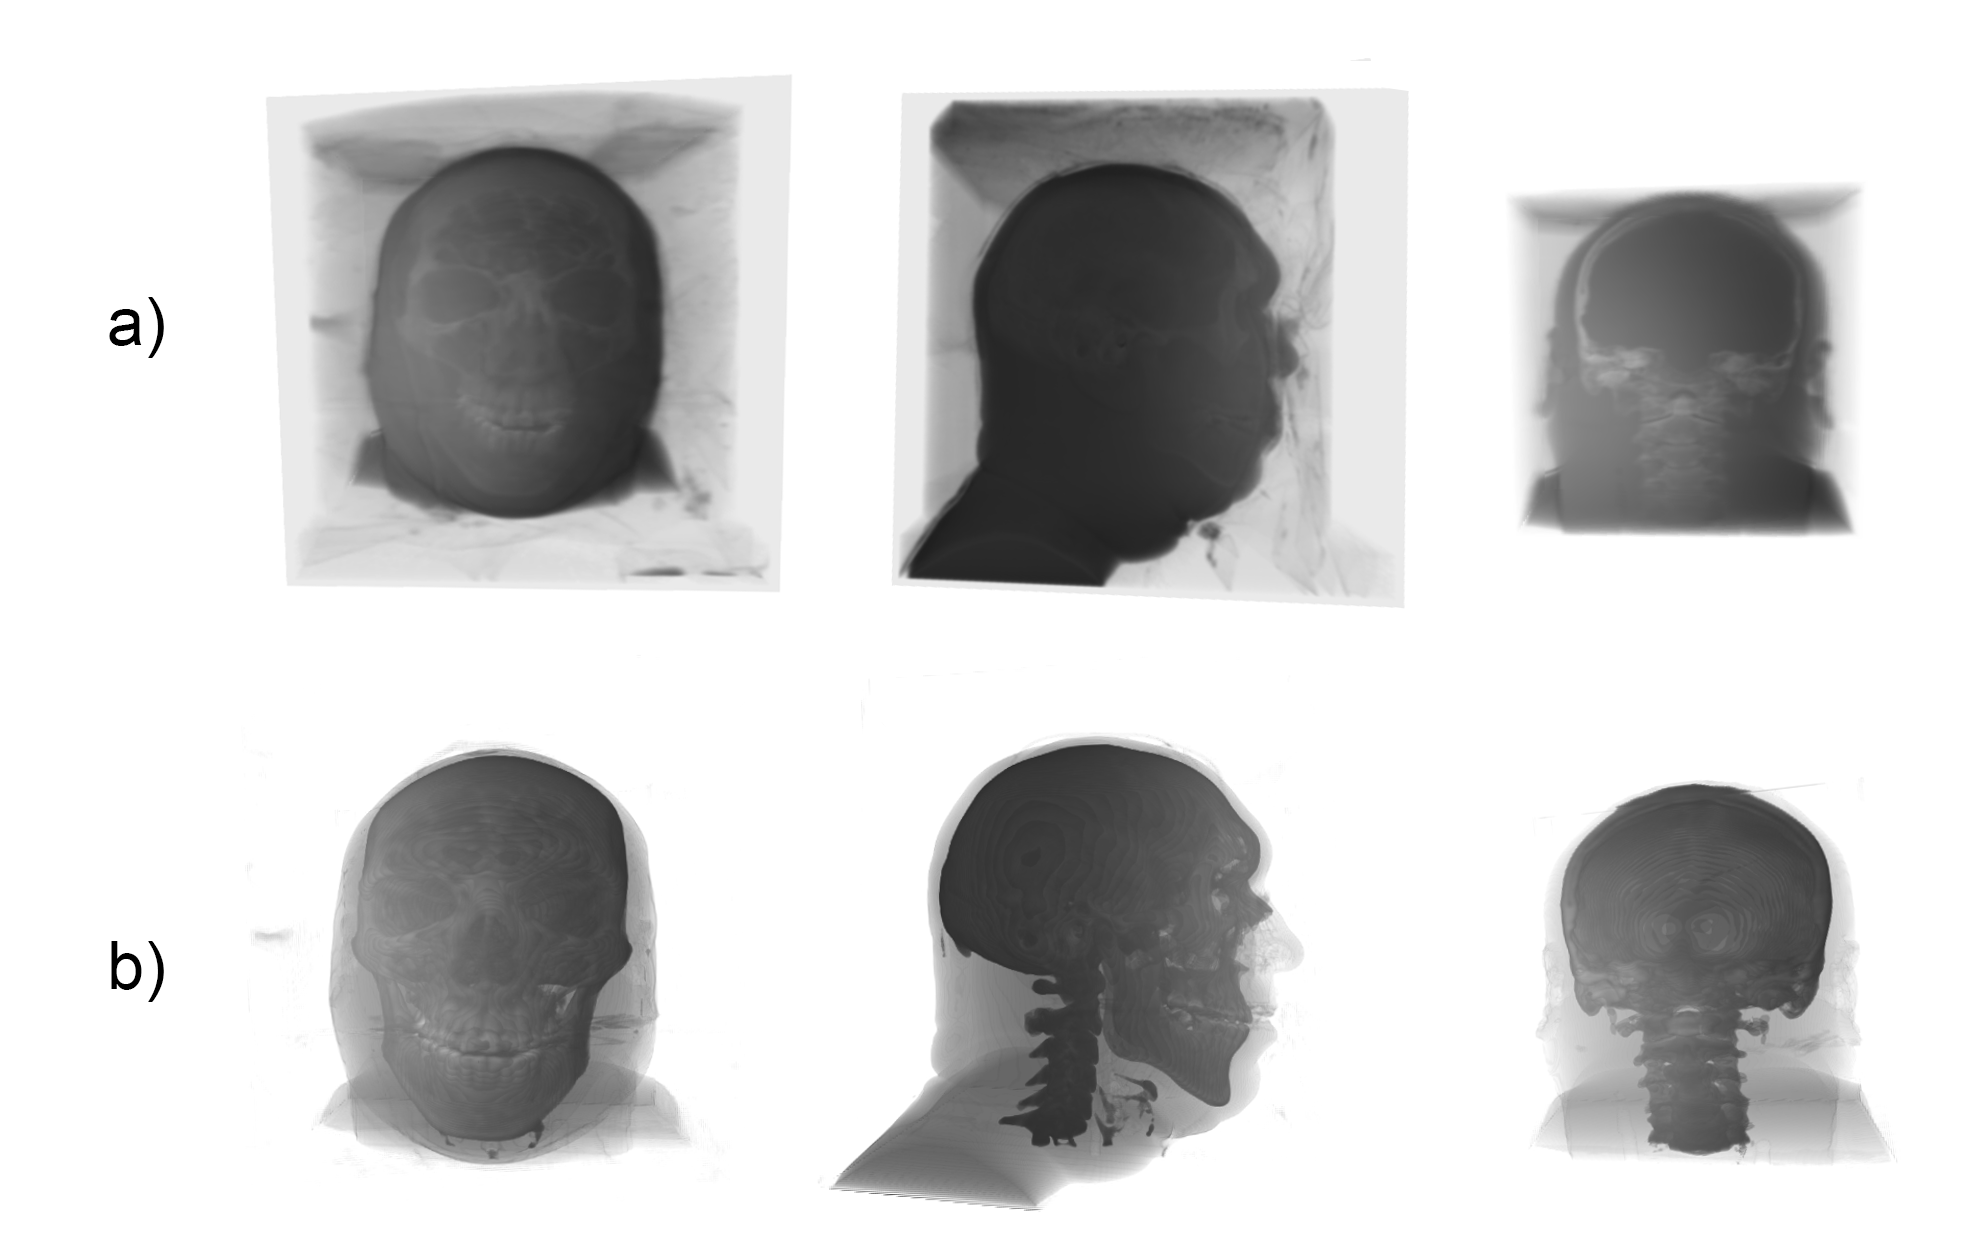
\includegraphics[width=0.9\linewidth]{images/visMale_result.png}
	\caption{Rendering eines alternativen Datensatzes durch den in mARt verwendeten Shader mit gleicher Intensität. a) Rendering ohne Transferfunktion b) Rendering mit Transferfunktion}
	\label{img:resultsVisMale}
	\source{Eigene Darstellung}
\end{figure}
\FloatBarrier

Der gekennzeichnete Bereich, der verdeutlicht welche Teile des Gehirns von dem Schlaganfall betroffen wurden, ist durch die semitransparente Darstellung von allen Seiten gut zu erkennen. 
Durch die Multiplikation der Masken- und Isowerte ist die Struktur des Gehirns weiterhin erkennbar. In Abbildung \ref{img:resultMask} sind Renderings des Gehirns und des Bereichs dargestellt.

\begin{figure}[!htb]
	\centering
	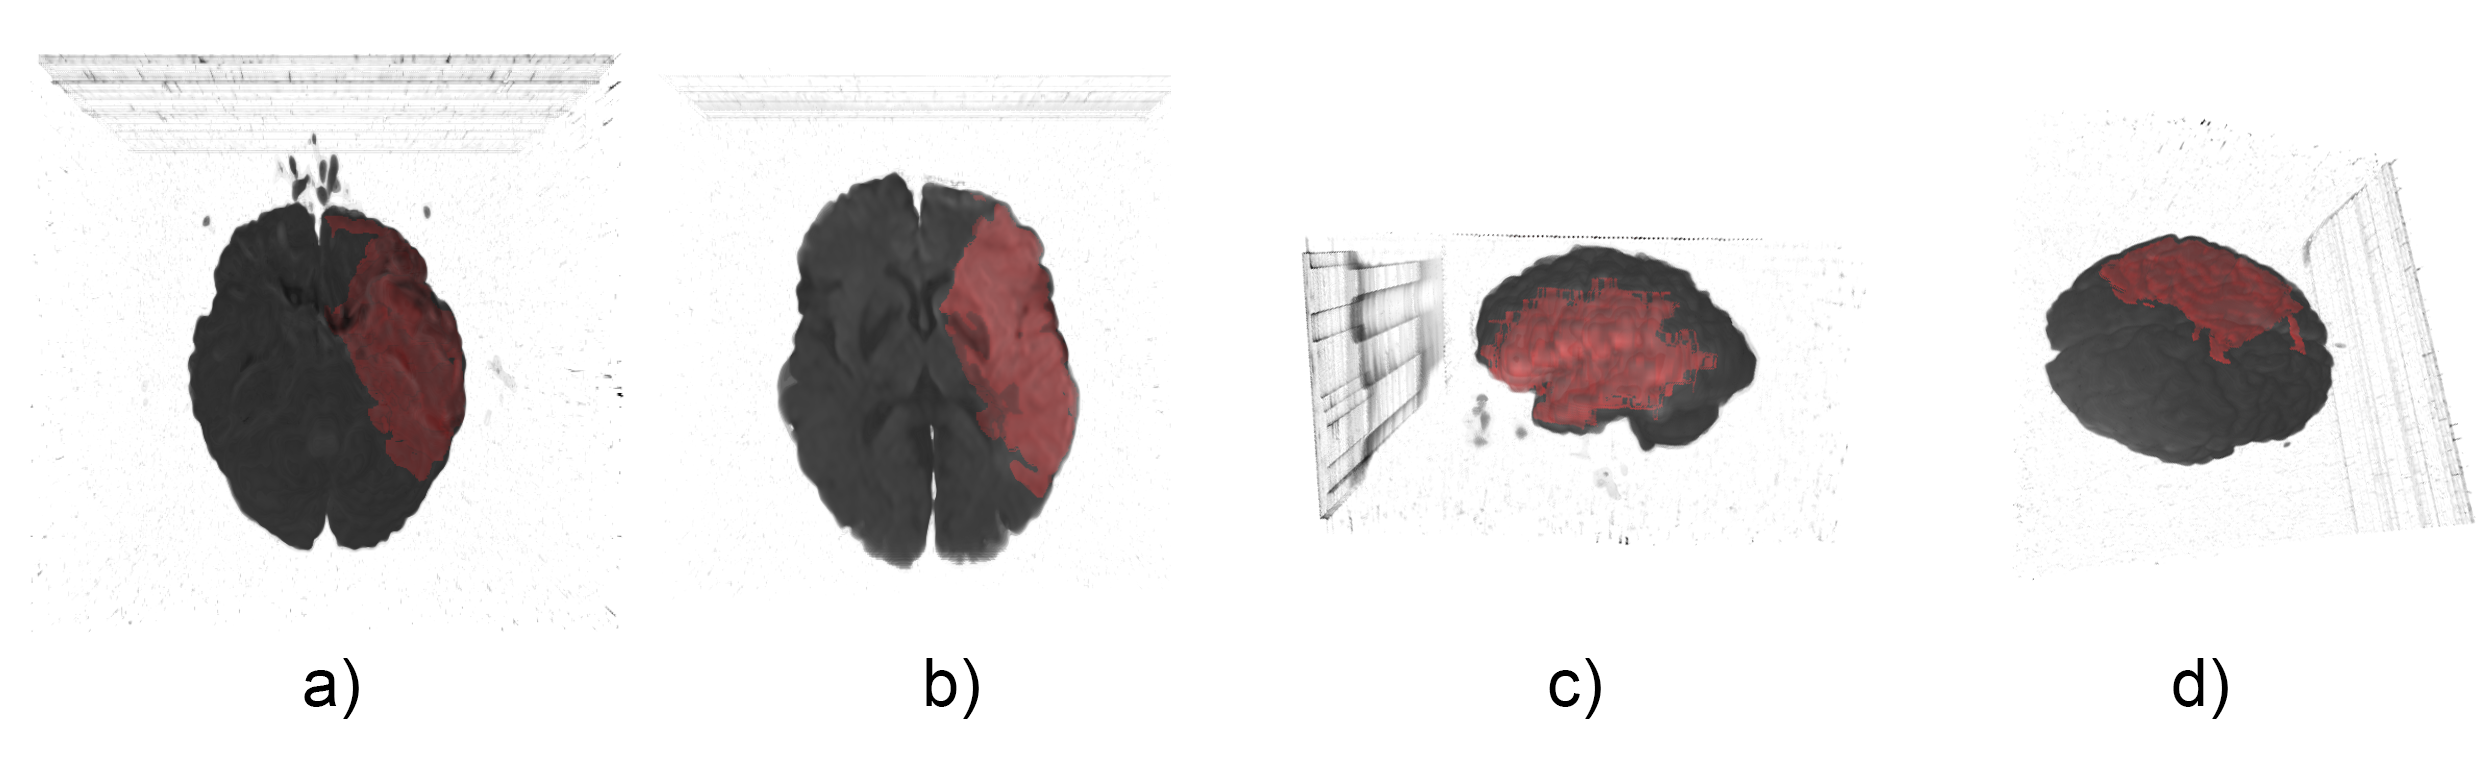
\includegraphics[width=0.99\linewidth]{images/mask_results.png}
	\caption{Rendering des ersten Datensatzes und der Maske, die den betroffenen Bereich hervorhebt, aus verschiedenen Ansichten.}
	\label{img:resultMask}
	\source{Eigene Darstellung}
\end{figure}
\FloatBarrier
  
\subsection{AR Anwendung}
Durch die semi-transparente Darstellung in AR sind die eher dunklen MRT-Daten teilweise schlecht zu erkennen. Dies betrifft vor allem die 3D-Darstellung. Um das Rendering erkennen zu können müssen die Farbwerte durch die Gammakorrektur erhellt werden. In Abbildungen \ref{img:ARLicht} und \ref{img:ARLicht3D} dargestellt, wie die Daten mit dem Standardhelligkeitswert und mit einem erhöhten Wert aussehen.

\begin{figure}[!htb]
	\centering
	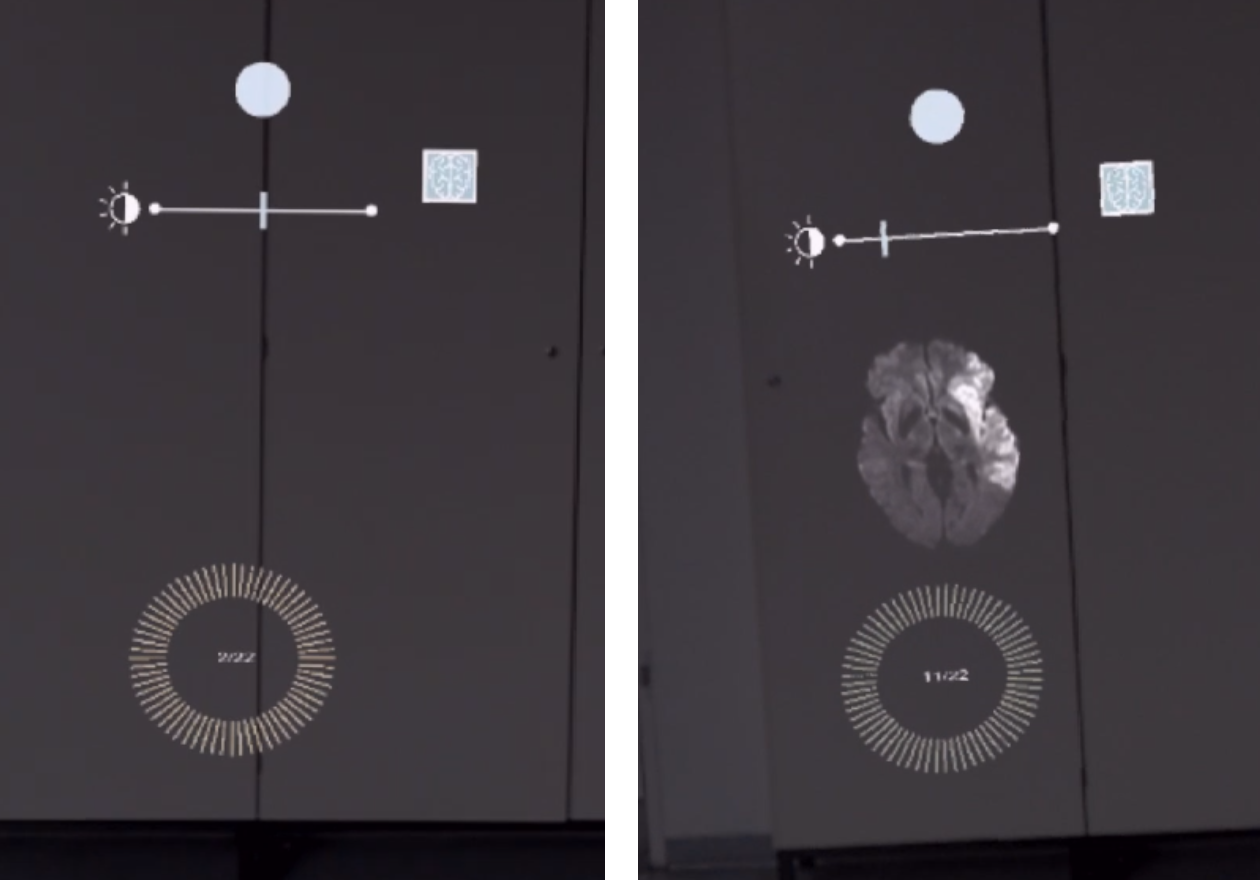
\includegraphics[width=0.7\linewidth]{images/mARt_AR_brightness.png}
	\caption{Zwei Aufnahmen aus der \textit{HoloLens}, während der 2D-Scene von mARt mit unverändertem (links) und erhöhtem (rechts) Gammakorrekturwert. Um die Darstellung erkennen zu können muss der Wert erhöht werden.}
	\label{img:ARLicht}
	\source{Eigene Darstellung}
\end{figure}
\FloatBarrier

\begin{figure}[!htb]
	\centering
	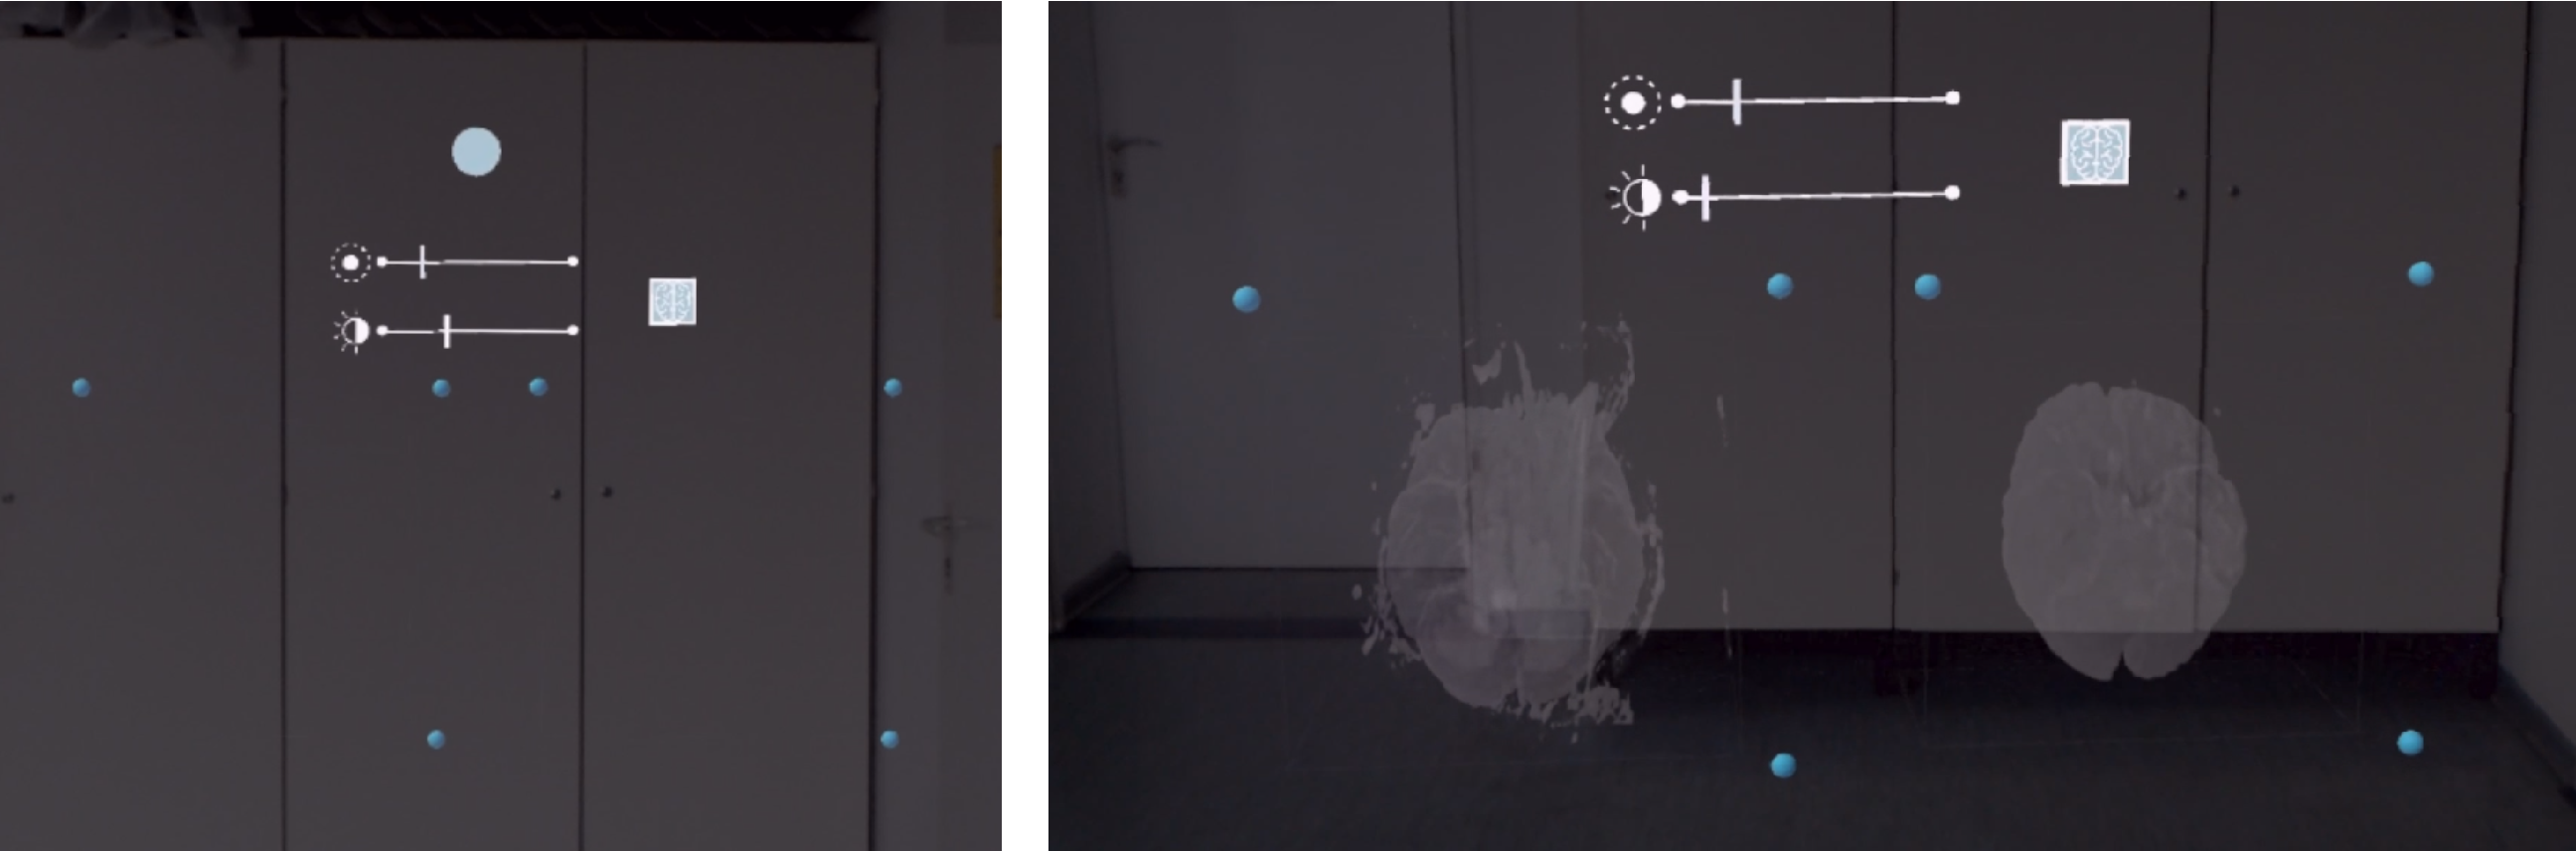
\includegraphics[width=0.9\linewidth]{images/mARt_AR_brightness_3D.png}
	\caption{Zwei Aufnahmen aus der \textit{HoloLens}, während der 3D-Scene von mARt mit unverändertem (links) und erhöhtem (rechts) Gammakorrekturwert. Um die Darstellung erkennen zu können muss der Wert erhöht werden.}
	\label{img:ARLicht3D}
	\source{Eigene Darstellung}
\end{figure}
\FloatBarrier

Ein weiterer Punkt, der die Verwendung der Anwendung auf der \textit{HoloLens} erschwert, ist das eingeschränkte Sichtfeld des Gerätes. Dieses Problem wurde bereit in Kapitel \ref{grundlagen} beschrieben. 
Die Begrenzung der Darstellung führt dazu, dass die MRT-Daten aus der Sicht des Nutzers meist abgeschnitten sind. Um die Daten gleichzeitig mit den Interaktionselementen sehen zu können, muss der Nutzer einen Abstand von ca. 1,5m zur Darstellung haben. Dies macht es ihm allerdings unmöglich mit dieser zu interagieren. Um die Darstellung manipulieren zu können, muss er also zwischen MRT-Bildern und Bedienelementen hin- und herblicken. In Abbildung \ref{img:ARCutoff} ist das abgeschnittene Sichtfeld der \textit{HoloLens} dargestellt. Dabei werden die virtuellen Hände des Nutzer nicht angezeigt, wenn er diese nicht direkt ansieht, auch wenn die Leap Motion diese vielleicht noch erfasst. 
Die Darstellung der Hände selbst nimmt bereits einen großen Teil des Sichtfeldes der \textit{HoloLens} ein, da sie sich nah am HMD befinden. 
Eine Bedienung der Anwendung auf der \textit{HoloLens} ist aus diesen Gründen sehr schwer. 

\begin{figure}[!htb]
	\centering
	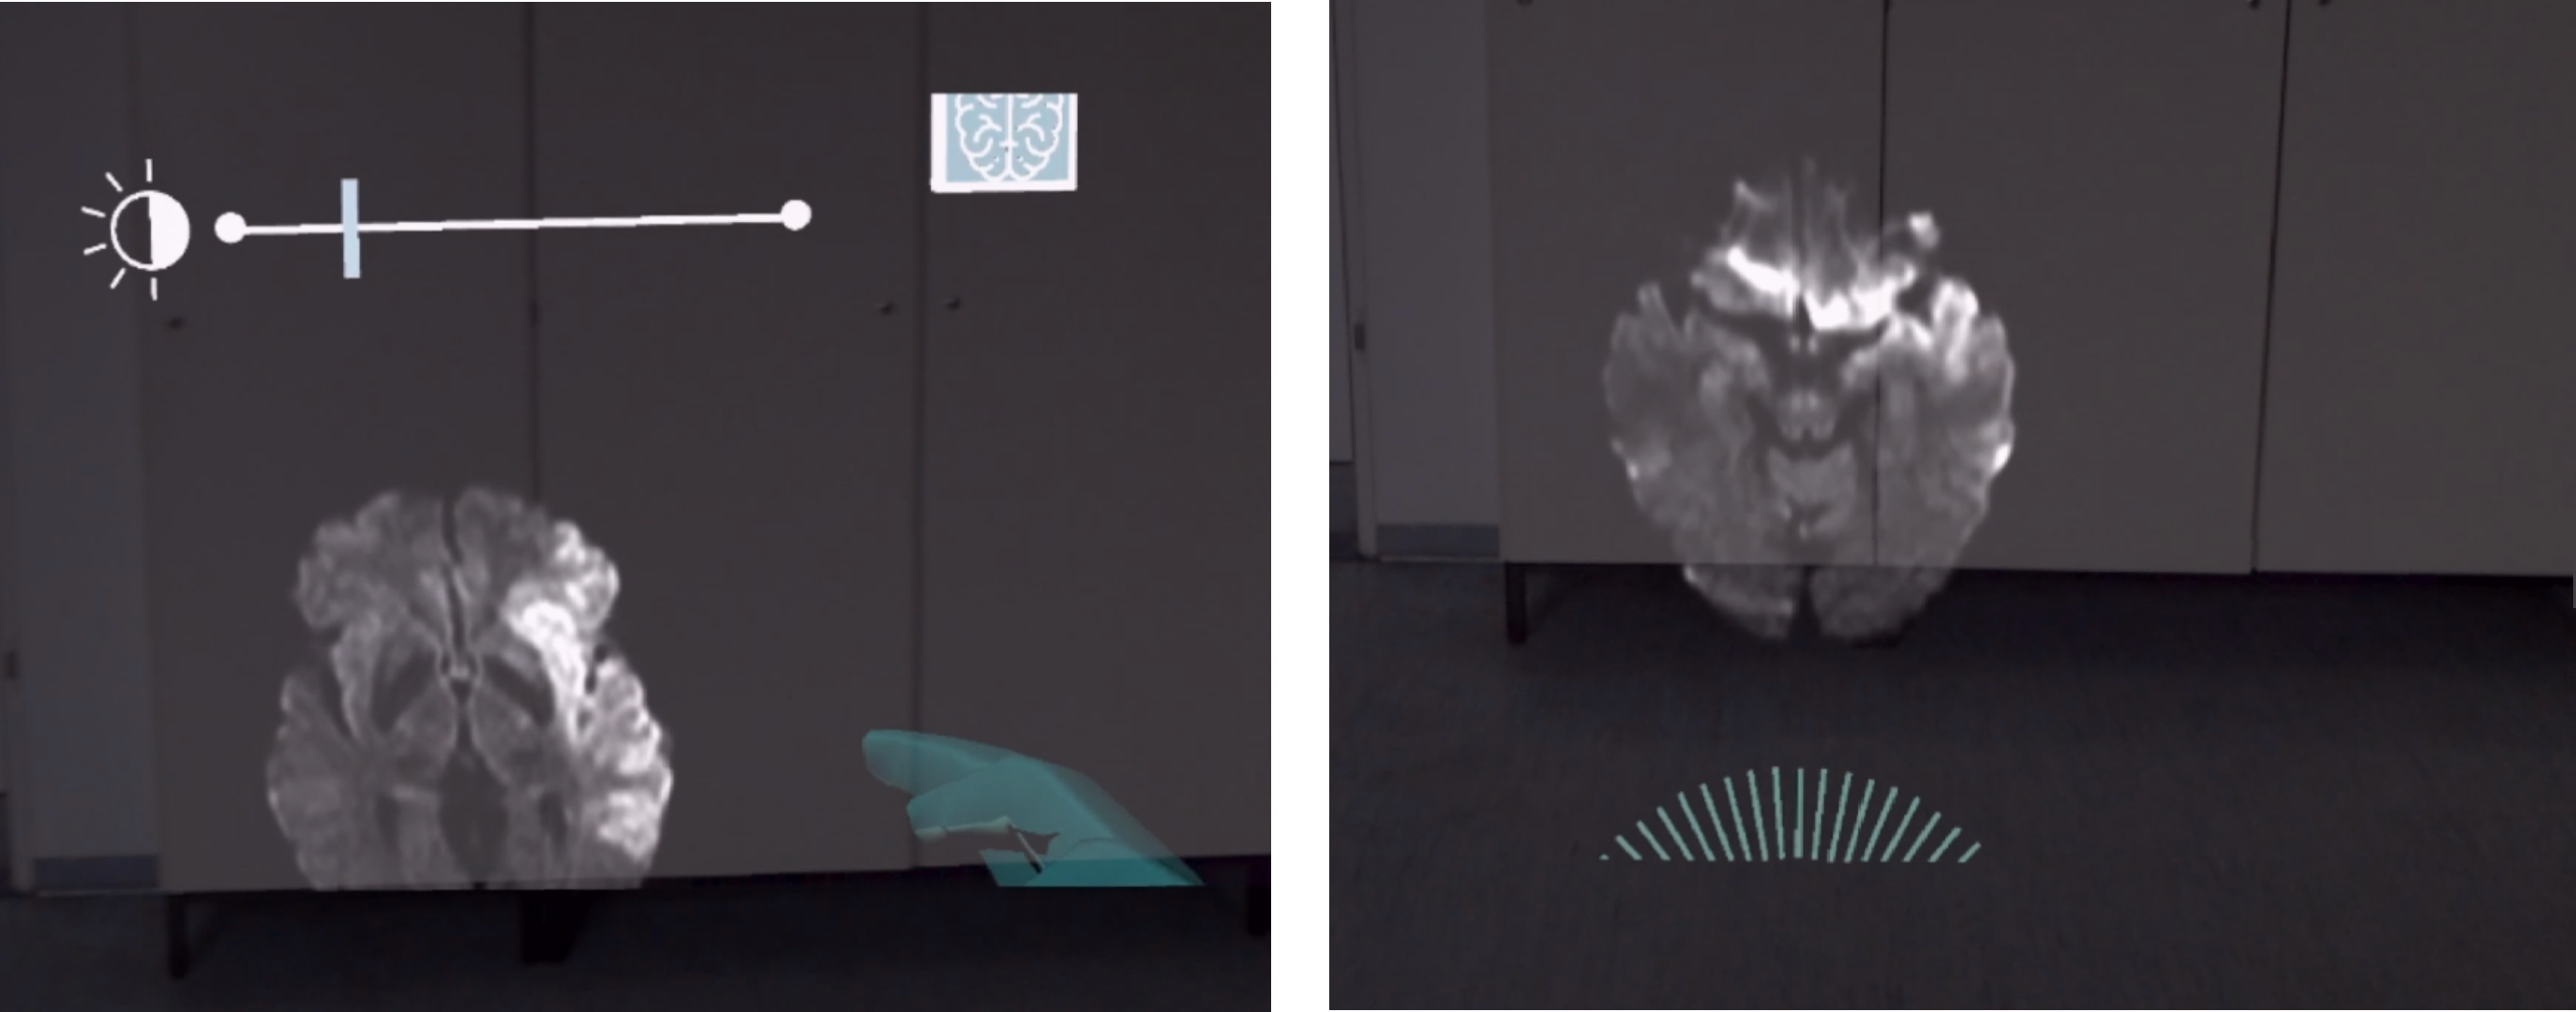
\includegraphics[width=0.9\linewidth]{images/mARt_Cutoff.png}
	\caption{Zwei Aufnahmen aus der \textit{HoloLens}, während der 2D-Scene von mARt aus bedienbarer Entfernung. Durch das begrenzte Sichtfeld der \textit{HoloLens} wir nur ein Ausschnitt der Anwendung dargestellt.}
	\label{img:ARCutoff}
	\source{Eigene Darstellung}
\end{figure}
\FloatBarrier


% Evaluation


\chapter{Evaluation}
\label{evaluation}

\section{Vergleich mit Anforderungen}

Zunächst werden in der folgenden Tabelle \ref{tab:evaluation} die implementierten Funktionen von mARt mit den in Kapitel \ref{anforderung} aufgestellten Anforderungen abgeglichen. Die Anforderung ist dabei über die entsprechende User Story referenziert. Dazu ist angegeben, inwiefern die Anforderung erfüllt wurde, so wie eventuelle Anmerkungen. 

\begin{longtable} {p{.125\textwidth}p{.225\textwidth}p{.60\textwidth}}
\toprule
User Story & Erfüllung & Anmerkungen \\
\toprule
U01 & Erfüllt & Die Darstellung der Daten ist zu großen Teilen abhängig von diesen selbst. Die Darstellung in AR ist abhängig von den Lichtverhältnissen.\\
\midrule 
U02 & Erfüllt & Die Betrachtung aus einem Winkel ist möglich.\\
\midrule 
U03 & Erfüllt & \\
\midrule 
U04 & Erfüllt & Die Anzahl der angezeigten Datensätze ist auf zwei beschränkt.\\
\midrule 
U05 & Erfüllt & Die Daten, aus denen der Nutzer wählen kann sind fest in das Programm integriert und es kann nur aus zwei Datensätzen gewählt werden.\\
\midrule
U06 & Erfüllt erfüllt & Maximal zwei Darstellungen können gleichzeitig manipuliert werden. \\
\midrule 
U07 & Erfüllt & Die zweidimensionale Darstellung kann auf einer Achse verändert werden. Die dreidimensionale auf drei.\\
\midrule 
U08 & Offen & \\
\midrule 
U09 & Erfüllt & \\
\midrule 
U10 & Teilweise erfüllt & Manipulationen außer Skalierung und Rotation werden übernommen, sofern der Wert in beiden Szenarien existiert.\\
\midrule 
U11  & Erfüllt & \\
\midrule
U12 & Erfüllt & Eine Manipulation der Maske würde dem Nutzer eine Anpassung erlauben, wurde jedoch nicht umgesetzt.\\
\midrule 
U13 & Erfüllt & \\
\midrule 
U14 & Erfüllt & \\
\midrule 
U15 & Erfüllt & Nur bei Anzeige eines Datensatzes möglich. Temporäte Manipulation.\\
\midrule 
U16 & Erfüllt & Die position wird nicht über mehrere Sitzungen hinweg gespeichert.\\
\midrule 
U17 & Offen & Nicht umsetzbar durch Abhängigkeit von einem PC.\\
\midrule 
U18 & Offen & Keine unterschiedlichen Sequenzen standen zur Verfügung.\\
\midrule 
U19 & Offen & Datensätze sind in Anwendung integriert.\\
\midrule 
U20 & Offen & Datensätze sind in Anwendung integriert.\\

\bottomrule
\caption{\label{tab:evaluation}Erfüllung der Anforderungen.}
\end{longtable}

\section{Nutzertest}

Um die Verwendung von mARt im Bereich der Schlaganfallbehandlung zu evaluieren wurde ein Nutzertest abgehalten. 
Dabei wurden sowohl die AR- als auch die VR-Anwendung von einem Neurologen getestet. 

Ergebnisse

\section{Auswertung}
% Was ist besser als vorher? Warum?
% Fazit

\chapter{Zusammenfassung und Fazit}
\label{fazit}

\section{Zusammenfassung}

Im Rahmen dieser Arbeit wurde untersucht, inwiefern eine interaktive dreidimensionale Darstellung von MRT-Daten in einer AR-Anwendung einen Mehrwert für Neurologen im Bereich der Behandlung von Schlaganfällen bietet. 
Hierzu wurden zunächst technische Hintergründe zu MRT-Daten, den Möglichkeiten der 3D-Darstellung von diesen sowie AR- und VR-Technologien erläutert. Weiterhin wurden damit in Zusammenhang stehende Arbeiten genannt. Einer der Schwerpunkte dieses Abschnitts war die Vorstellung verschiedener Volume Rendering Techniken.

Als Grundlage zur Konzeption der AR-Anwendung wurden dann Anforderungen aufgestellt, die durch Interviews mit einem Neurologen der Charité Berlin erarbeitet wurden. Diese wurden als User Stories formuliert.

Anschließend wurde diskutiert, wie die einzelnen Funktionalitäten von mARt umgesetzt werden können. Hierbei wurden sowohl Aspekte der Implementierung als auch der Gestaltung von Bedienelementen und Aussehen der Anwendung berücksichtigt. Unter anderem wurden aus den zuvor beschriebenen Techniken die geeignetsten ausgewählt. 

Das beschriebene Konzept wurde implementiert und einzelne relevante Punkte der Umsetzung wurden erläutert. Die Ergebnisse der Implementierung wurden präsentiert.

Schließlich wurde die Anwendung mit den zuvor aufgestellten Anforderungen abgeglichen und von einem Neurologen getestet. 
Es konnte gezeigt werden, dass die Darstellung der dreidimensionalen Daten im Raum zu einem besseren Verständnis der Situation führt. Die direkte Interaktion mit der Darstellung trägt dazu bei. 

\section{Ausblick}

Wie mehrfach beschrieben wurde, handelt es sich bei mARt primär um einen Prototyp, der die Vorteile des Einsatzes einer AR-Anwendung zur Darstellung von MRT-Daten untersucht. Dementsprechend existieren viele Möglichkeiten das Programm in verschieden Richtungen zu erweitern.
Im Folgenden werden einige mögliche weiterführerende Entwicklungen von mARt erläutert.

\subsection{Implementierung offener  Anforderungen}

Wie im Kapitel \ref{evaluation} dargelegt wurde, konnte nicht alle anfangs gestellten Anforderungen im Rahmen dieser Arbeit umgesetzt werden. Um mARt für den Einsatz im Arbeitsumfeld nutzbar zu machen sollten diese erfüllt sein.

%U08
In User Story \textbf{U08} wird ein Scrollrad für den Wechsel zwischen den Schichten gefordert. Da die Steuerung von mARt im Rahmen dieser Arbeit allerdings durch Gesten erfolgt, wurde sie nicht erfüllt. In zukünftigen Konzepten lässt sich die Gestensteuerung allerdings möglicherweise mit anderen Bedienelementen kombinieren, beispielsweise einem Scrollrad, das multifunktional verwendet wird. Dies ist allerdings abhängig von dem angestrebten Anwendungsfall.

%U10 (teilweise)
Weiterhin wurde durch Story \textbf{U10} ein Wechsel zwischen 2D- und 3D-Darstellung beschrieben, bei dem die vom Nutzer getätigten Manipulationen in das jeweils andere Szenario übertragen werden. Diese Anforderung wurde nur teilweise erfüllt. Wie in Kapitel \ref{konzept} erläutert wurde, sind manche Manipulationen, wie die Skalierung nur temporär. In einem veränderten Konzept einer AR-Anwendung wie mARt, können sich Möglichkeiten ergeben alle Manipulationen zu übertragen oder sogar die Darstellungen synchron anzuzeigen.

%U17
Die in Story \textbf{U17} geforderte dauerhafte Positionierung im Raum wurde ebenfalls nur teilweise umgesetzt. Die Darstellung kann im Raum platziert werden. Allerdings behält sie diese Position nicht über mehrere Sitzungen hinweg. 
Weiterhin ist ihre Position relativ zur Position des Nutzers. Für den Prototyp ist dies ausreichend. Die User Story hat ihren Ursprung allerdings in der Idee einer Multiuser-Anwendung. Dabei können mehrere Nutzer die selbe Darstellung betrachten, die sich für alle an der selben Position im Raum befindet. Dieses Konzept wurde in Kapitel \ref{konzept} erläutert. Vor allem für Einsätze demonstrativer Art, wie Lernzwecke oder die Kommunikation mit Patienten wäre diese Funktion von Nutzen.

%U18
Eine weitere unerfüllte User Story ist \textit{U18}, die beschreibt, dass möglichst alle Sequenzen eines Scans eines Patienten wählbar sein sollen. Für diese Arbeit wurden nur eine begrenzte Anzahl an Datensätzen zur Verfügung gestellt. Bei der Untersuchung eines möglichen Schlaganfalls, kommen allerdings oft verschiedene Scans und Gewichtungen zum Einsatz, wie in Abschnitt \ref{mrt} beschrieben wurde. Sollten mehrere Datensätze zu einem Patienten vorliegen, ist es sinnvoll aus diesen wählen zu können. Dies steht allerdings in Zusammenhang mit der Implementierung einer generellen Auswahl von Daten, aus denen der Nutzer wählen kann, wie sie bereits dargelegt wurde.

%U19-20
Wie ebenfalls in Kapitel \ref{konzept} erläutert wurde, unterstützt der Prototyp nicht die Darstellung von vom Nutzer gewählten Dateien. Dementsprechend werden auch keine Dateien im DICOM- oder NIfTI-Format unterstützt. Für die Nutzung von Neurologen oder auch erweiterte Tests ist diese Funktion allerdings notwendig. Dazu müsste im Konzept der Anwendung eine Möglichkeit gefunden werden dem Nutzer die Auswahl von Daten zu erlauben und diese in das Programm zu übertragen. Dies setzt unter anderem voraus, dass ein Parser integriert wird, der die Daten aus besagten Formaten in einen für \textit{Unity} lesbaren Typ umwandelt. 

Hinzu kommen die Erweiterungen, die in Abschnitt \ref{nutzertest} beschrieben wurden. 
Abhängig von den konkreten Nutzungsszenarien werden sich außerdem weitere Anforderungen ergeben, um die mARt erweitert bzw. an die es angepasst werden muss. 
Es wäre wünschenswert, dass diese sowie zukünftige ähnliche Arbeiten einem Test mit einer größeren Anzahl an Testern unterzogen wird, da dies noch mehr Aufschluss über die Bedürfnisse verschiedener Nutzer und die Möglichkeiten einer AR-Anwendung liefert.

\subsection{Verbesserte 3D Visualisierung}

Die Ergebnisse des Volume Rendering der MRT-Daten wurde in Abschnitt \ref{ergebnisse} demonstriert. Der Nutzertest hat gezeigt, dass die Darstellungen von ausreichender Qualität sind, um eine Diagnose durchzuführen und vor allem den Zustand des Gehirns nach einen Schlaganfall zu vermitteln. 
Allerdings stellt das Volume Rendering für sich einen eigenen Forschungsbereich dar, der im Rahmen dieser Arbeit nicht abgedeckt werden konnte. Darin existieren viele Maßnahmen, um die Qualität der Darstellung weiter zu verbessern. Einige davon werden an dieser Stelle genannt. 

Zum einen wurde als Rendering Verfahren das Volume RayCasting gewählt, da es sehr gute Ergebnisse liefert. Je nachdem in welche Richtung sich zukünftige Arbeiten entwickeln, ist es allerdings sinnvoll weitere Verfahren zu testen, die beispielsweise weniger rechenintensiv sind. 
Weiterhin wurde zwar eine Transferfunktion verwendet, um das Rauschen der Bilder zu beschränken. Allerdings ist diese nicht für jeden Datensatz optimal und es wird lediglich ihr Alphawert genutzt. 
Idealerweise sollte dem Nutzer die Möglichkeit gegeben werden die Transferfunktion zu beeinflussen, wie es in Kapitel \ref{konzept} bereits erläutert wurde. Dies würde die Darstellungsqualität erhöhen und dem Nutzer zu einem Rendering nach seinen Ansprüchen verhelfen. 
Um das Rendering plastischer und realer erscheinen zu lassen kann außerdem ein globales Beleuchtungsmodell implementiert werden, wie es in Kapitel \ref{grundlagen} beschrieben ist. 
Da die Qualität des Renderings von den Bilddaten abhängt, können diese schließlich bereinigt bzw. aufgearbeitet werden. Wie in Abschnitt \ref{ergebnisse} dargelegt wurde, besteht in den gegebenen Datensätzen ein hohes Maß an Rauschen. Dieses könnte auf verschiedenen Wegen herausgefiltert werden, bevor die Bilder gerendert werden. Zudem könnte eine zusätzliche Interpolation vorgenommen werden, die die großen Abstände zwischen den einzelnen Schichten besser überbrückt als es bisher der Fall ist. Damit könnten Bildartefakte reduziert werden. 
Für die Verbesserung der MRT-Daten könnte beispielsweise maschinelles Lernen eingesetzt werden.

\subsection{Übertragen der Anwendung auf andere Hardware}
\label{hololens2Fazit}

Im Rahmen dieser Arbeit wurde mARt als AR-Anwendung nur auf der \textit{HoloLens} getestet. 
Die Verwendung der Anwendung zusammen mit anderen AR-Systemen, könnte noch mehr Aufschluss über die Möglichkeiten von AR-Systemen im medizinischen Bereich geben. 
mARt könnte dabei auf vergleichbaren AR-Systemen, wie der \textit{Magic Leap} von \cite{magicLeap} getestet werden.
Da die Entwicklung solcher Systeme momentan weiter fortschreitet, kommen allerdings auch noch nicht erschienene Geräte in Betracht.

Wie im Kapitel \ref{evaluation} beschreiben wurde, ist die Interaktion mit mARt durch das geringe Sichtfeld der \textit{HoloLens} erschwert. Die Inhalte werden abgeschnitten und die virtuellen Hände nehmen viel Platz ein. 
Dieses und andere Probleme, die bei der Verwendung von mARt auf der \textit{HoloLens} festgestellt wurden, könnten eventuell durch die Verwendung auf der \textit{HoloLens 2} behoben werden. 
Das Gerät wurde im Februar 2019 vorgestellt und soll voraussichtlich im April 2019 erscheinen. 
Die neue Version der \textit{HoloLens} besitzt ein mehr als doppelt so großes Sichtfeld, wie ihr Vorgänger (vgl. \cite{hololens2}), was dem eben genannten Problem entgegen wirkt. 
Weiterhin verfügt die \textit{HoloLens 2} über eine eingebaute Hand-Tracking-Funktion (vgl. \cite{hololens2}). Diese könnte an Stelle der \textit{Leap Motion} zum Erfassen der Hände des Nutzers verwendet werden. Dadurch entstehen zwei Vorteile gegenüber der aktuellen Anwendung. Zum Einen ist anzunehmen, dass die virtuellen Hände nicht länger angezeigt werden müssen. Dies vereinfacht die Benutzung und lässt mehr Raum im Sichtfeld für tatsächliche Inhalte. Zum Anderen, könnte die Anwendung für die \textit{HoloLens 2} bereitgestellt und somit kabellos verwendet werden, wodurch die Verzögerung der Übertragung auf das Gerät behoben und das Nutzungserlebnis verbessert würden. 

Weiterhin ist davon auszugehen, dass die \textit{HoloLens 2} über eine höhere Rechenleistung verfügt, als ihr Vorgänger. Dies könnte neben der eben genannten Optimierung des Renderingverfahrens eine flüssige Darstellung der 3D-MRT-Daten ermöglichen.

Eine Übertragung der Anwendung auf die \textit{HoloLens 2} könnte die Benutzbarkeit der Anwendung demnach stark erhöhen.

\subsection{Integration anderer Technologien}

Im vorherigen Abschnitt wurde bereits der Einsatz von maschinellem Lernen zur Verbesserung der Bildqualität angeführt. Diese Technologie könnte weiterhin zur Diagnose von Schlaganfällen oder zur Prognose ihrer Entwicklung verwendet werden. Funktionen dieser Art könnten in Anwendungen wie mARt  integriert werden.
\todo{Paper? P}

\section{Fazit}

Die Motivation hinter dieser Arbeit war es zu untersuchen, inwiefern eine interaktive AR-Anwendung die Untersuchung von volumetrischen MRT-Daten verbessern kann. Obwohl der dafür entworfene Prototyp längst nicht den Umfang eines MRT-Viewers abdeckt, konnten Schlüsse über die Möglichkeiten einer solchen Anwendung gezogen werden.
Der Nutzertest hat gezeigt, dass mARt zu einem besseren Verständnis der Situation führen kann. Dies wird durch die dreidimensionale Darstellung im Raum sowie die direkte Interaktion mit den Daten erreicht.
Eine AR-Anwendung dieser Art besitzt enormes Potenzial Nutzer in verschiedenen Anwendungsfällen zu unterstützen. Dazu gehört die Arbeit von Neurologen aber auch anderen Ärzten, sowie das Studium von Medizinstudenten und die Kommunikation mit Patienten. 

Bis AR-Anwendungen wie mARt Alltagsrealität werden bedarf es allerdings noch weiterer Entwicklungen.
Der derzeitige Stand der AR-Technologie stellt dabei das größte Hindernis dar. Wie in der Arbeit gezeigt werden konnte, ist die Darstellung von Volumendaten ein weitreichend erforschtes Gebiet. Um eine solche Darstellung über ein HMD in einer interaktiven Anwendung zur Verfügung zu stellen, muss dieses drei Voraussetzungen erfüllen:

\begin{itemize}
\item Die Leistung muss ausreichen, um hochwertige Renderings durchzuführen.
\item Es müssen intuitive und bequeme Interaktionsmöglichkeiten verfügbar sein.
\item Der Tragekomfort sollte eine Benutzung über einen längeren Zeitraum ermöglichen.
\end{itemize}

All dies trifft momentan nicht auf AR-HMDs wie die \textit{HoloLens} zu. Es ist wahrscheinlich, dass zukünftige Systeme der ständig voranschreitenden Technologie diese Eigenschaften mitbringen werden. 
Bis dahin gilt es zu untersuchen, was die notwendigen Interaktionen und relevantes Elemente für die jeweiligen Anwendungsfälle sind und wie diese sinnvoll in AR realisiert werden können, damit eine stabile und einsetzbare Anwendung entstehen kann, die das dargelegte Potenzial ausschöpft.
mARt ist somit der erste Schritt einer Entwicklung, um die Arbeit und Zusammenarbeit von Ärzten, Studenten und Patienten zu bereichern.



\pagebreak

\printbibliography

\end{document}
